\documentclass[12pt, a4paper]{article}

% ------- Packages -------
\usepackage[utf8]{inputenc}
\usepackage[T1]{fontenc}
\usepackage[english]{babel}
\usepackage{geometry}
\usepackage{graphicx}
\usepackage{float}
\usepackage{booktabs}
\usepackage{longtable}
\usepackage{array}
\usepackage{tabularx}
\usepackage{multirow}
\usepackage{xcolor}
\usepackage{listings}
\usepackage{caption}
\usepackage{subcaption}
\usepackage{hyperref}
\usepackage{fancyhdr}
\usepackage{titlesec}
\usepackage{enumitem}
\usepackage{amsmath}
\usepackage{amssymb}
\usepackage{tikz}
\usepackage{mdframed}
\usepackage{setspace}
\usepackage{parskip}
\usepackage{pdfpages}
\usepackage{xurl}
\usetikzlibrary{calc}

% ------- Page geometry --------
\geometry{
    a4paper,
    top=2cm,
    bottom=2cm,
    left=2.5cm,
    right=2cm
}

% ------- Colors -------
\definecolor{primaryblue}{RGB}{30, 100, 200}
\definecolor{codegreen}{RGB}{40, 140, 60}
\definecolor{codegray}{RGB}{120, 120, 120}
\definecolor{codebg}{RGB}{248, 248, 248}
\definecolor{codestring}{RGB}{180, 50, 50}
\definecolor{sectioncolor}{RGB}{20, 80, 160}
\definecolor{lightblue}{RGB}{230, 240, 255}
\definecolor{warnyellow}{RGB}{255, 250, 220}
\definecolor{successgreen}{RGB}{220, 245, 225}

% ------- Listings (code style) -------
\lstdefinestyle{sqlstyle}{
    language=SQL,
    backgroundcolor=\color{codebg},
    commentstyle=\color{codegray}\itshape,
    keywordstyle=\color{primaryblue}\bfseries,
    stringstyle=\color{codestring},
    basicstyle=\ttfamily\small,
    breakatwhitespace=false,
    breaklines=true,
    captionpos=b,
    keepspaces=true,
    numbers=left,
    numbersep=8pt,
    numberstyle=\tiny\color{codegray},
    showstringspaces=false,
    tabsize=2,
    frame=single,
    rulecolor=\color{gray!40},
    xleftmargin=1.5em,
}

\lstdefinestyle{pythonstyle}{
    language=Python,
    backgroundcolor=\color{codebg},
    commentstyle=\color{codegreen}\itshape,
    keywordstyle=\color{primaryblue}\bfseries,
    stringstyle=\color{codestring},
    basicstyle=\ttfamily\small,
    breaklines=true,
    captionpos=b,
    numbers=left,
    numbersep=8pt,
    numberstyle=\tiny\color{codegray},
    showstringspaces=false,
    tabsize=4,
    frame=single,
    rulecolor=\color{gray!40},
    xleftmargin=1.5em,
}

% ------- Section formatting -------
\titleformat{\section}[block]
  {\Large\bfseries\color{sectioncolor}}
  {\thesection}{0.8em}{}[\titlerule]

\titleformat{\subsection}[block]
  {\large\bfseries\color{sectioncolor!80}}
  {\thesubsection}{0.6em}{}

\titleformat{\subsubsection}[block]
  {\normalsize\bfseries}
  {\thesubsubsection}{0.5em}{}

% ------- Header / Footer -------
\pagestyle{fancy}
\fancyhf{}
\fancyhead[L]{\small\textit{Personal Finance Management System}}
\fancyfoot[C]{\thepage}
\renewcommand{\headrulewidth}{0.4pt}

% ------- Hyperref -------
\hypersetup{
    colorlinks=true,
    linkcolor=primaryblue,
    urlcolor=primaryblue,
    citecolor=primaryblue,
    pdftitle={Personal Finance Management System},
    pdfauthor={Student Report},
}

% ------- Custom environments -------
\newmdenv[
  backgroundcolor=lightblue,
  linecolor=primaryblue,
  linewidth=1.5pt,
  roundcorner=4pt,
  innertopmargin=8pt,
  innerbottommargin=8pt,
  innerleftmargin=12pt,
]{infobox}

\newmdenv[
  backgroundcolor=successgreen,
  linecolor=codegreen,
  linewidth=1.5pt,
  roundcorner=4pt,
  innertopmargin=8pt,
  innerbottommargin=8pt,
  innerleftmargin=12pt,
]{successbox}

% ============================================================
\begin{document}
% ============================================================

\hyphenpenalty=10000
\exhyphenpenalty=10000
\sloppy

% ------- Cover Page -------
\begin{titlepage}
\newgeometry{top=2cm, bottom=2cm, left=3cm, right=2cm}

\begin{tikzpicture}[remember picture, overlay]
    \draw[line width = 2pt, color=sectioncolor]
        ($(current page.north west) + (2.0cm,-1.5cm)$)
        rectangle ($(current page.south east) + (-1.5cm,1.5cm)$);
    \draw[line width = 0.5pt, color=sectioncolor]
        ($(current page.north west) + (2.15cm,-1.65cm)$)
        rectangle ($(current page.south east) + (-1.65cm,1.65cm)$);
\end{tikzpicture}

\begin{center}
    {\fontsize{14}{16}\selectfont\textbf{NATIONAL ECONOMICS UNIVERSITY}}\\[0.3cm]
    {\fontsize{12}{15}\selectfont\textbf{Mathematics Faculty of Economics}}\\[0.2cm]
    \rule{0.4\textwidth}{1pt}

    \vspace{1.2cm}

    
\includegraphics[width=6.5cm, keepaspectratio=true]{logo.jpg}

    \vspace{1.2cm}

    {\fontsize{18}{22}\selectfont\bfseries\color{sectioncolor} FINAL PROJECT}\\[0.5em]
    {\fontsize{15}{18}\selectfont\bfseries DATABASE MANAGEMENT SYSTEMS}

    \vspace{1.2cm}

    {\fontsize{14}{17}\selectfont\bfseries PROJECT 13} \\[0.5cm]
    \begin{spacing}{1.5}
        {\fontsize{20}{26}\selectfont\bfseries\color{sectioncolor}
        PERSONAL FINANCE\\
        MANAGEMENT SYSTEM}
    \end{spacing}

    \vspace{1.2cm}

    \begin{flushleft}
      \hspace{4cm}
      \begin{tabular}{@{}l@{\hspace{0.5cm}:\hspace{0.4cm}}l@{}}
          {\fontsize{15}{20}\selectfont Student}
              & {\fontsize{15}{20}\selectfont\bfseries Nguyen Phuong Ngan} \\[0.6em]
          {\fontsize{15}{20}\selectfont Class}
              & {\fontsize{15}{20}\selectfont\bfseries DSEB 66B} \\[0.6em]
          {\fontsize{15}{20}\selectfont Student ID}
              & {\fontsize{15}{20}\selectfont\bfseries 11245914} \\[0.6em]
          {\fontsize{15}{20}\selectfont Instructor}
              & {\fontsize{15}{20}\selectfont\bfseries PhD. Tran Hung} \\
      \end{tabular}
    \end{flushleft}

    \vfill

    {\fontsize{13}{18}\selectfont\bfseries Hanoi, \the\month/\the\year}

\end{center}
\restoregeometry
\end{titlepage}

% ------- Attach project brief -------
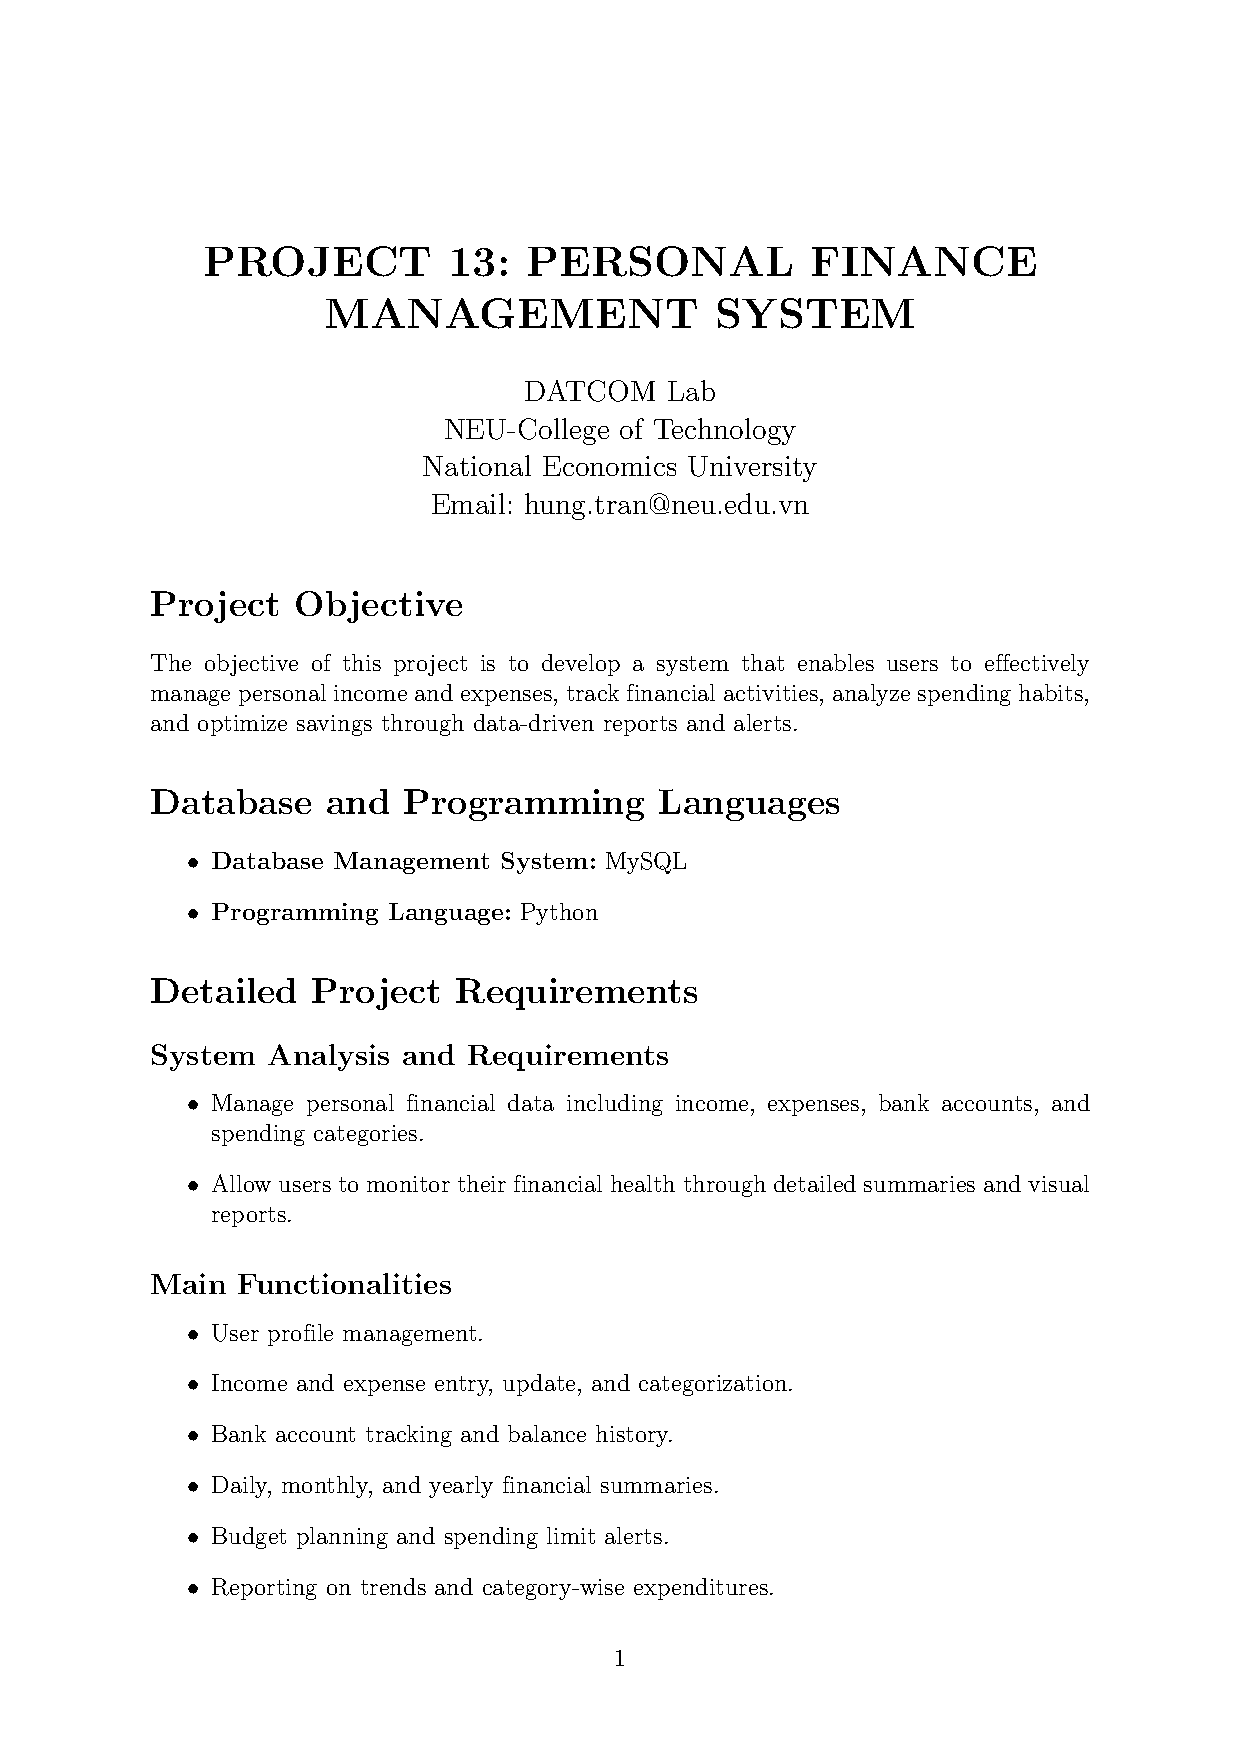
\includepdf[pages=1-3, pagecommand={\thispagestyle{empty}}]{Topic.pdf}

% ------- TOC -------
\setcounter{tocdepth}{2}
\tableofcontents
\newpage

% ============================================================
\section{Problem Understanding and Requirement Analysis}
% ============================================================

\subsection{Problem Statement}

Managing personal finances is a persistent challenge for individuals, particularly young
professionals and students in Vietnam, where cash-based transactions remain common and
awareness of structured budgeting is limited. Without a centralised system, people
frequently lose track of their spending patterns, miss budget thresholds, and struggle to
identify which expense categories are draining their income.

This project addresses that gap by building a \textbf{Personal Finance Management System
(PFMS)} -- a desktop application backed by a relational database -- that enables users
to record income and expenses, monitor bank account balances in real time, set spending
budgets per category, and analyse their financial behaviour through visual reports.

\subsection{Objectives}

The system is designed to achieve the following objectives:

\begin{enumerate}[leftmargin=2em]
  \item Provide a persistent, structured data store for all financial transactions using
        MySQL, exploiting advanced database features (triggers, stored procedures, views,
        UDFs) to enforce business rules at the database layer.
  \item Deliver an intuitive desktop graphical interface (CustomTkinter) that allows
        non-technical users to record transactions, manage budgets, and view analytics
        without writing any SQL.
  \item Demonstrate the practical value of database-level automation: bank account
        balances must always reflect the sum of all income minus all expenses, enforced
        by a full lifecycle set of six triggers rather than application code, so data
        integrity is guaranteed regardless of how the database is accessed.
  \item Produce actionable financial insights through two reporting modes: a
        \textbf{Performance Snapshots} tab presenting daily, monthly, and yearly
        numerical summaries side-by-side; and a \textbf{Visual Analytics} tab
        containing three interactive chart types -- income-versus-expenses bar chart,
        category-spending pie chart, and cumulative balance trend line chart -- with
        hover tooltips displaying exact VND values.
\end{enumerate}

\subsection{Scope}

\begin{infobox}
\textbf{In scope:} User profile management (create and edit); bank account tracking;
income and expense entry, editing, and deletion with full trigger-driven balance
adjustment; monthly budget setting, updating, and deletion; three graphical reports
with interactive tooltips; daily, monthly, and yearly performance snapshots; database
security via role-restricted MySQL user; automated balance updates via six triggers.\\[0.5em]
\textbf{Out of scope:} Mobile application; integration with real banking APIs;
multi-currency support; cloud synchronisation; collaborative (multi-device) access.
\end{infobox}

\subsection{Inputs and Outputs}

\begin{table}[H]
\centering
\caption{System Inputs and Outputs}
\begin{tabularx}{\textwidth}{>{\bfseries}lX}
\toprule
\textbf{Direction} & \textbf{Description} \\
\midrule
\textbf{Inputs}
& User profile data (name, email, phone); bank account details (bank name,
  initial balance); income records (amount, date, account, description);
  expense records (amount, category, account, date, description); budget
  limits (category, month, maximum amount); edit and delete requests for
  existing income, expense, and budget records. \\
\addlinespace
\textbf{Outputs}
& Real-time account balance (updated automatically by trigger);
  daily income/expense totals via \texttt{CURDATE()} query;
  monthly income/expense summary; yearly net savings aggregate;
  budget utilisation status with WARNING/EXCEEDED alerts;
  three interactive matplotlib charts with hover tooltips embedded in the UI;
  monthly closure snapshot via stored procedure. \\
\bottomrule
\end{tabularx}
\end{table}

\subsection{Functional Requirements}

\begin{table}[H]
\centering
\caption{Functional Requirements}
\begin{tabularx}{\textwidth}{clX}
\toprule
\textbf{ID} & \textbf{Priority} & \textbf{Requirement} \\
\midrule
FR-01 & Must & The system shall maintain a Users table with unique email addresses. \\
FR-02 & Must & Each user may have multiple bank accounts; balance must equal the running
               total of income minus expenses for that account. \\
FR-03 & Must & Every income insertion shall automatically increment the linked bank account
               balance (via trigger). \\
FR-04 & Must & Every expense insertion shall automatically decrement the linked bank account
               balance (via trigger); balance must not fall below zero. \\
FR-05 & Must & Users shall be able to set a monthly spending budget per expense category;
               budgets may also be deleted when no longer needed. \\
FR-06 & Must & The system shall calculate budget utilisation percentage and flag status as
               OK / WARNING (${\geq}$80\%) / EXCEEDED (${\geq}$100\%). \\
FR-07 & Must & Monthly income-vs-expense reports shall be generated using a database view. \\
FR-08 & Must & A stored procedure shall return a full monthly financial report for a user. \\
FR-09 & Should & UDFs shall encapsulate total-expense and budget-usage calculations for
                 reuse in SQL queries. \\
FR-10 & Should & The Python GUI shall provide four screens: Dashboard, Transactions,
                 Reports, Budgets. \\
FR-11 & Must & The system shall provide daily financial summaries (today's income and
               expenses) and yearly aggregates for the selected year, displayed
               alongside monthly figures in the Reports screen. \\
FR-12 & Should & Users shall be able to perform full CRUD operations on income and expense
                 records; edits and deletions shall trigger automatic balance adjustments
                 via database triggers. \\
FR-13 & Should & Users shall be able to create new expense categories inline from the
                 Add Expense form, and update their own profile information from the
                 sidebar. \\
\bottomrule
\end{tabularx}
\end{table}

\subsection{Non-Functional Requirements}

\begin{itemize}[leftmargin=2em]
  \item \textbf{Data integrity:} All foreign key relationships enforce referential
        integrity with \texttt{ON DELETE CASCADE} where appropriate. Check constraints
        prevent negative amounts and malformed email addresses.
  \item \textbf{Security:} The Python application connects to MySQL using a restricted
        user (\texttt{finance\_app}) that holds only SELECT, INSERT, UPDATE, DELETE (on
        transaction tables), and EXECUTE privileges -- no DROP or structural DDL.
  \item \textbf{Performance:} Composite indexes on \texttt{(UserID, ExpenseDate)} and
        \texttt{(UserID, IncomeDate)} ensure sub-millisecond filtering on typical dataset
        sizes.
  \item \textbf{Maintainability:} Code is split into \texttt{db\_connection.py},
        \texttt{models.py}, \texttt{reports.py}, and \texttt{main.py}, following a
        separation-of-concerns architecture. The UI layer contains zero SQL strings.
\end{itemize}

\newpage

% ============================================================
\section{Design and Technical Soundness}
% ============================================================

\subsection{System Architecture}

The Personal Finance Management System follows a structured three-layer architecture
to ensure modularity and security. This design separates the user interface from the
data management logic, as illustrated in Figure~\ref{fig:system_architecture}.

\begin{figure}[htbp]
  \centering
  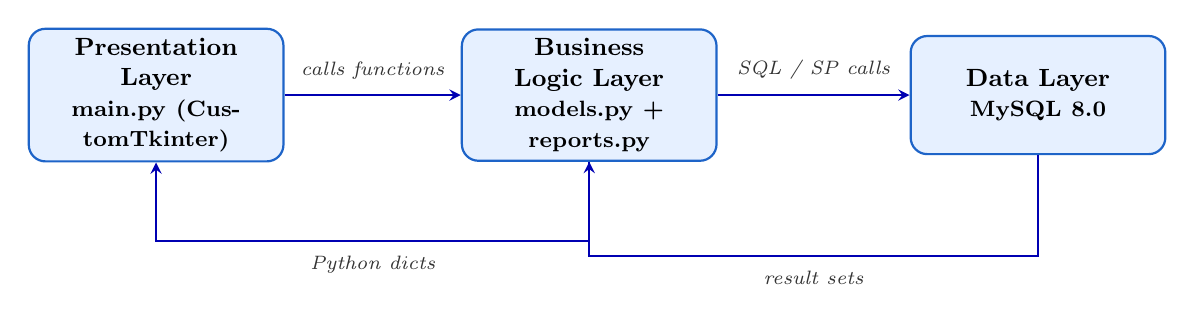
\begin{tikzpicture}[
    box/.style={rectangle, rounded corners=6pt, draw=primaryblue, fill=lightblue,
                text width=3.0cm, minimum height=1.5cm, align=center,
                font=\small\bfseries, thick},
    arrow/.style={->, >=stealth, thick, color=blue!70!black},
    label_font/.style={font=\scriptsize\itshape, color=black!80}
  ]
    \node[box] (ui) at (0,0)    {Presentation Layer\\{\footnotesize main.py (CustomTkinter)}};
    \node[box] (bl) at (5.5,0)  {Business Logic Layer\\{\footnotesize models.py + reports.py}};
    \node[box] (db) at (11.2,0) {Data Layer\\{\footnotesize MySQL 8.0}};

    \draw[arrow] (ui.east) -- node[midway, above, label_font, yshift=2pt]{calls functions} (bl.west);
    \draw[arrow] (bl.east) -- node[midway, above, label_font, yshift=2pt]{SQL / SP calls} (db.west);
    \draw[arrow] (db.south) -- ++(0,-1.275) -| node[pos=0.25, below, label_font, yshift=-2pt]{result sets} (bl.south);
    \draw[arrow] (bl.south) -- ++(0,-1.0)   -| node[pos=0.25, below, label_font, yshift=-2pt]{Python dicts} (ui.south);
  \end{tikzpicture}
  \caption{System architecture showing the interaction between UI, logic, and database layers.}
  \label{fig:system_architecture}
\end{figure}

\textbf{Design rationale:} The UI layer is strictly decoupled from the database,
meaning it never contains raw SQL strings. All data interactions are routed through
\texttt{models.py} using parameterised queries or stored procedures. Chart generation
is handled exclusively by \texttt{reports.py}, which calls \texttt{models.py} functions
to retrieve data and returns \texttt{matplotlib} \texttt{Figure} objects that
\texttt{main.py} embeds via \texttt{FigureCanvasTkAgg}. Interactive tooltips are
implemented by registering \texttt{motion\_notify\_event} callbacks in \texttt{main.py}
against hidden annotation objects pre-built inside each chart. This architecture makes
SQL injection structurally impossible from the presentation layer and ensures that
schema changes only necessitate updates in a single localised file.

\subsection{Entity-Relationship Design}

The data model comprises six entities. The cardinalities and relationships are
summarised below:

\begin{table}[H]
\centering
\caption{Entity Relationships}
\begin{tabularx}{\textwidth}{llX}
\toprule
\textbf{Entity A} & \textbf{Entity B} & \textbf{Relationship} \\
\midrule
Users             & BankAccounts       & One-to-Many (a user owns multiple accounts) \\
Users             & Income             & One-to-Many (a user records multiple income entries) \\
Users             & Expenses           & One-to-Many (a user records multiple expenses) \\
Users             & Budgets            & One-to-Many (a user sets budgets per month/category) \\
BankAccounts      & Income             & One-to-Many (income is deposited into one account) \\
BankAccounts      & Expenses           & One-to-Many (expenses are deducted from one account) \\
ExpenseCategories & Expenses           & One-to-Many (each expense belongs to one category) \\
ExpenseCategories & Budgets            & One-to-Many (budgets are set per category) \\
\bottomrule
\end{tabularx}
\end{table}

\begin{figure}[H]
  \centering
  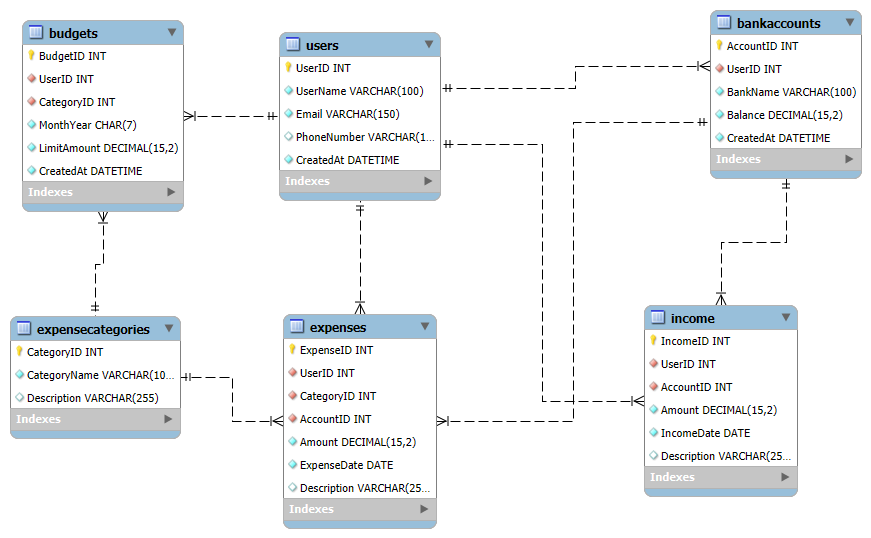
\includegraphics[width=0.92\textwidth]{ERD.png}
  \caption{ER Diagram}
\end{figure}

\subsection{Relational Schema}

\subsubsection{Table: Users}
\begin{table}[H]
\centering
\caption{Users Table Structure}
\begin{tabularx}{\textwidth}{lllX}
\toprule
\textbf{Column} & \textbf{Data Type} & \textbf{Constraints} & \textbf{Description} \\
\midrule
UserID      & INT           & PK, AUTO\_INCREMENT & Surrogate primary key \\
UserName    & VARCHAR(100)  & NOT NULL            & Full display name \\
Email       & VARCHAR(150)  & NOT NULL, UNIQUE    & Login identifier; CHECK format \\
PhoneNumber & VARCHAR(15)   & --                  & Optional contact number \\
CreatedAt   & DATETIME      & DEFAULT NOW()       & Account creation timestamp \\
\bottomrule
\end{tabularx}
\end{table}

\subsubsection{Table: BankAccounts}
\begin{table}[H]
\centering
\caption{BankAccounts Table Structure}
\begin{tabularx}{\textwidth}{lllX}
\toprule
\textbf{Column} & \textbf{Data Type} & \textbf{Constraints} & \textbf{Description} \\
\midrule
AccountID & INT           & PK, AUTO\_INCREMENT      & Surrogate primary key \\
UserID    & INT           & FK $\to$ Users, NOT NULL & Account owner \\
BankName  & VARCHAR(100)  & NOT NULL                 & Name of the bank \\
Balance   & DECIMAL(15,2) & DEFAULT 0, CHECK $\geq$0 & Current balance; auto-updated by triggers \\
CreatedAt & DATETIME      & DEFAULT NOW()            & Account opening timestamp \\
\bottomrule
\end{tabularx}
\end{table}

\subsubsection{Table: Income}
\begin{table}[H]
\centering
\caption{Income Table Structure}
\begin{tabular}{llll}
\toprule
\textbf{Column} & \textbf{Data Type} & \textbf{Constraints} & \textbf{Description} \\
\midrule
IncomeID    & INT           & PK, AUTO\_INCREMENT   & Surrogate primary key \\
UserID      & INT           & FK $\to$ Users        & Income recipient \\
AccountID   & INT           & FK $\to$ BankAccounts & Target account \\
Amount      & DECIMAL(15,2) & NOT NULL, CHECK $>0$  & Income amount in VND \\
IncomeDate  & DATE          & NOT NULL              & Date received \\
Description & VARCHAR(255)  & --                    & Optional note \\
\bottomrule
\end{tabular}
\end{table}

\subsubsection{Table: ExpenseCategories}
\begin{table}[H]
\centering
\caption{ExpenseCategories Table Structure}
\begin{tabularx}{\textwidth}{lllX}
\toprule
\textbf{Column} & \textbf{Data Type} & \textbf{Constraints} & \textbf{Description} \\
\midrule
CategoryID   & INT          & PK, AUTO\_INCREMENT & Surrogate primary key \\
CategoryName & VARCHAR(100) & NOT NULL, UNIQUE    & e.g.\ Food \& Dining, Transport \\
Description  & VARCHAR(255) & --                  & Optional category description \\
\bottomrule
\end{tabularx}
\end{table}

\subsubsection{Table: Expenses}
\begin{table}[H]
\centering
\caption{Expenses Table Structure}
\begin{tabular}{llll}
\toprule
\textbf{Column} & \textbf{Data Type} & \textbf{Constraints} & \textbf{Description} \\
\midrule
ExpenseID   & INT           & PK, AUTO\_INCREMENT        & Surrogate primary key \\
UserID      & INT           & FK $\to$ Users             & Spender \\
CategoryID  & INT           & FK $\to$ ExpenseCategories & Spending classification \\
AccountID   & INT           & FK $\to$ BankAccounts      & Source account \\
Amount      & DECIMAL(15,2) & NOT NULL, CHECK $>0$       & Expense amount in VND \\
ExpenseDate & DATE          & NOT NULL                   & Date of expense \\
Description & VARCHAR(255)  & --                         & Optional note \\
\bottomrule
\end{tabular}
\end{table}

\subsubsection{Table: Budgets}
\begin{table}[H]
\centering
\caption{Budgets Table Structure}
\begin{tabularx}{\textwidth}{lllX}
\toprule
\textbf{Column} & \textbf{Data Type} & \textbf{Constraints} & \textbf{Description} \\
\midrule
BudgetID    & INT           & PK, AUTO\_INCREMENT        & Surrogate primary key \\
UserID      & INT           & FK $\to$ Users             & Budget owner \\
CategoryID  & INT           & FK $\to$ ExpenseCategories & Budget category \\
MonthYear   & CHAR(7)       & NOT NULL (format YYYY-MM)  & Budget month \\
LimitAmount & DECIMAL(15,2) & NOT NULL, CHECK $>0$       & Monthly spending ceiling \\
CreatedAt   & DATETIME      & DEFAULT NOW()              & Creation timestamp \\
\bottomrule
\end{tabularx}
\end{table}

\subsection{Advanced Database Objects}

\subsubsection{Indexes}

Three composite indexes were created to optimise the most frequent query patterns:

\begin{lstlisting}[style=sqlstyle, caption={Index Definitions}]
-- Speeds up: "Show expenses for user X in month Y"
CREATE INDEX idx_expenses_user_date
    ON Expenses(UserID, ExpenseDate);

-- Speeds up: "Show income for user X in month Y"
CREATE INDEX idx_income_user_date
    ON Income(UserID, IncomeDate);

-- Speeds up: budget utilisation checks per user/category/month
CREATE INDEX idx_budgets_user_cat_month
    ON Budgets(UserID, CategoryID, MonthYear);
\end{lstlisting}

\textbf{Justification:} Without these indexes, every monthly filter would require a
full table scan. With a B-tree index on \texttt{(UserID, ExpenseDate)}, MySQL can seek
directly to the relevant rows in $O(\log n)$ time.

\subsubsection{Views}

The system utilizes database views to abstract complex \texttt{JOIN} logic and
multi-level aggregations into reusable virtual tables. This ensures that the Python
application remains database-agnostic for its reporting needs, fetching pre-calculated
results via simple \texttt{SELECT} statements.

\paragraph{1. Monthly Financial Overview (\texttt{vw\_monthly\_summary})}

This view provides the primary data for the monthly bar charts. Because MySQL 8.0 does
not natively support \texttt{FULL OUTER JOIN}, a \texttt{UNION} of a \texttt{LEFT JOIN}
and a \texttt{RIGHT JOIN} is implemented to ensure months with only income or only
expenses are never omitted.

\begin{lstlisting}[style=sqlstyle, caption={vw\_monthly\_summary View (excerpt)}]
CREATE OR REPLACE VIEW vw_monthly_summary AS
SELECT 
    u.UserID, u.UserName, summary.MonthYear, 
    summary.TotalIncome, summary.TotalExpenses,
    (summary.TotalIncome - summary.TotalExpenses) AS NetSavings
FROM Users u
JOIN (
    SELECT 
        COALESCE(inc.UserID, exp.UserID) AS UserID,
        COALESCE(inc.MonthYear, exp.MonthYear) AS MonthYear,
        COALESCE(inc.TotalIncome, 0) AS TotalIncome,
        COALESCE(exp.TotalExpenses, 0) AS TotalExpenses
    FROM (
        -- Aggregate Income by User and Month
        SELECT UserID, DATE_FORMAT(IncomeDate, '%Y-%m') 
            AS MonthYear, SUM(Amount) AS TotalIncome 
        FROM Income GROUP BY UserID, MonthYear
    ) inc
    LEFT JOIN (
        -- Aggregate Expenses by User and Month
        SELECT UserID, DATE_FORMAT(ExpenseDate, '%Y-%m') 
            AS MonthYear, SUM(Amount) AS TotalExpenses 
        FROM Expenses GROUP BY UserID, MonthYear
    ) exp ON inc.UserID = exp.UserID 
            AND inc.MonthYear = exp.MonthYear
    
    UNION -- Ensure months with only expenses are included
    
    SELECT 
        COALESCE(inc.UserID, exp.UserID) AS UserID,
        COALESCE(inc.MonthYear, exp.MonthYear) AS MonthYear,
        COALESCE(inc.TotalIncome, 0) AS TotalIncome,
        COALESCE(exp.TotalExpenses, 0) AS TotalExpenses
    FROM (
        SELECT UserID, DATE_FORMAT(IncomeDate, '%Y-%m') 
            AS MonthYear, SUM(Amount) AS TotalIncome 
        FROM Income GROUP BY UserID, MonthYear
    ) inc
    RIGHT JOIN (
        SELECT UserID, DATE_FORMAT(ExpenseDate, '%Y-%m') 
            AS MonthYear, SUM(Amount) AS TotalExpenses 
        FROM Expenses GROUP BY UserID, MonthYear
    ) exp ON inc.UserID = exp.UserID 
            AND inc.MonthYear = exp.MonthYear
) summary ON u.UserID = summary.UserID;
\end{lstlisting}

\paragraph{2. Category-wise Spending (\texttt{vw\_category\_spending})}

This view breaks down expenditures by category for each user per month.
It simplifies data retrieval for \texttt{reports.py} to generate pie charts
without re-calculating sums in Python.

\begin{lstlisting}[style=sqlstyle, caption={vw\_category\_spending View}]
CREATE OR REPLACE VIEW vw_category_spending AS
SELECT
    e.UserID, u.UserName, ec.CategoryID, ec.CategoryName,
    DATE_FORMAT(e.ExpenseDate, '%Y-%m')     AS MonthYear,
    SUM(e.Amount)                           AS TotalSpent,
    COUNT(e.ExpenseID)                      AS TransactionCount
FROM Expenses e
JOIN Users u             ON e.UserID     = u.UserID
JOIN ExpenseCategories ec ON e.CategoryID = ec.CategoryID
GROUP BY e.UserID, u.UserName, ec.CategoryID, 
         ec.CategoryName, MonthYear;
\end{lstlisting}

\paragraph{3. Budget Performance Tracking (\texttt{vw\_budget\_status})}

This view compares budget limits to actual expenditures and encapsulates the system's
core business logic -- categorising financial health into three tiers:
\texttt{OK}, \texttt{WARNING}, and \texttt{EXCEEDED}.

\begin{lstlisting}[style=sqlstyle, caption={vw\_budget\_status View (excerpt)}]
CREATE OR REPLACE VIEW vw_budget_status AS
SELECT
    b.BudgetID, b.UserID, b.CategoryID, u.UserName,
    ec.CategoryName, b.MonthYear, b.LimitAmount,
    COALESCE(spent.TotalSpent, 0) AS SpentAmount,
    b.LimitAmount - COALESCE(spent.TotalSpent, 0) 
        AS RemainingAmount,
    ROUND(
        COALESCE(spent.TotalSpent, 0) / b.LimitAmount * 100, 2)
            AS UsagePercent,
    CASE
        WHEN COALESCE(spent.TotalSpent, 0) >= b.LimitAmount 
            THEN 'EXCEEDED'
        WHEN COALESCE(spent.TotalSpent, 0) >= b.LimitAmount*0.8 
            THEN 'WARNING'
        ELSE 'OK'
    END AS BudgetStatus
FROM Budgets b
JOIN Users u              ON b.UserID     = u.UserID
JOIN ExpenseCategories ec ON b.CategoryID = ec.CategoryID
LEFT JOIN (
    -- Subquery to get total spent per user/category/month
    SELECT UserID, CategoryID, DATE_FORMAT(ExpenseDate, '%Y-%m') 
        AS MonthYear, SUM(Amount) AS TotalSpent
    FROM Expenses GROUP BY UserID, CategoryID, MonthYear
) spent ON b.UserID = spent.UserID 
        AND b.CategoryID = spent.CategoryID 
        AND b.MonthYear = spent.MonthYear;
\end{lstlisting}

\paragraph{Summary of Database Views}

\begin{table}[H]
\centering
\caption{Database Views Technical Analysis}
\label{tab:database_views}
\begin{tabularx}{\textwidth}{lX}
\toprule
\textbf{View Name} & \textbf{Technical Purpose and Application Link} \\
\midrule
\texttt{vw\_monthly\_summary}   & Aggregates net savings by simulating a \texttt{FULL JOIN}.
                                  Used by \texttt{reports.py} for the bar chart and by
                                  \texttt{get\_yearly\_summary()} for yearly aggregation. \\
\texttt{vw\_category\_spending} & Groups transactions by category per month.
                                  Provides the data source for the category pie chart. \\
\texttt{vw\_budget\_status}     & Computes real-time budget utilisation percentages and
                                  status labels. Powers both the Budgets screen and the
                                  Dashboard alerts panel. \\
\bottomrule
\end{tabularx}
\end{table}

\textbf{Technical Analysis:} By leveraging subqueries within these views, the system
avoids Cartesian Product errors where joining multiple transaction rows might lead to
inflated sums. The use of \texttt{COALESCE} ensures data robustness, allowing the
system to handle months or categories with zero activity without returning \texttt{NULL}
values to the Python layer.

\subsubsection{User-Defined Functions}

Three UDFs encapsulate repetitive calculations that can be integrated into
\texttt{SELECT} statements and other database objects.

\begin{lstlisting}[style=sqlstyle, caption={UDF: fn\_get\_budget\_usage\_percent}]
CREATE FUNCTION fn_get_budget_usage_percent(
    p_UserID        INT,
    p_CategoryID    INT,
    p_MonthYear     CHAR(7)
)
RETURNS DECIMAL(5, 2)
READS SQL DATA
DETERMINISTIC
BEGIN
    DECLARE v_spent     DECIMAL(15, 2) DEFAULT 0.00;
    DECLARE v_limit     DECIMAL(15, 2) DEFAULT 0.00;
    DECLARE v_start_date DATE;
    SET v_start_date = STR_TO_DATE(CONCAT(p_MonthYear, '-01'), 
                                          '%Y-%m-%d');

    -- Get actual spending this month in this category
    SELECT COALESCE(SUM(Amount), 0)
    INTO   v_spent
    FROM   Expenses
    WHERE  UserID     = p_UserID
        AND  CategoryID = p_CategoryID
        AND  ExpenseDate >= v_start_date 
        AND  ExpenseDate <  DATE_ADD(v_start_date, 
                                     INTERVAL 1 MONTH);

    -- Get the budget limit
    SELECT COALESCE(LimitAmount, 0)
    INTO   v_limit
    FROM   Budgets
    WHERE  UserID     = p_UserID
        AND  CategoryID = p_CategoryID
        AND  MonthYear  = p_MonthYear
    LIMIT 1;

    -- Avoid division by zero
    IF v_limit = 0 THEN
        RETURN 0.00;
    END IF;

    RETURN ROUND((v_spent / v_limit) * 100, 2);
END;
\end{lstlisting}

\begin{table}[H]
\centering
\caption{User-Defined Functions Analysis}
\label{tab:udfs}
\begin{tabularx}{\textwidth}{>{\raggedright\arraybackslash}p{5.5cm} l X}
\toprule
\textbf{Function} & \textbf{Returns} & \textbf{Description} \\
\midrule
\texttt{fn\_get\_total\_income} \newline \footnotesize (UserID, MonthYear)
  & DECIMAL & Calculates total income for a user in a specific month; used in
             stored procedures for net savings calculations. \\
\addlinespace
\texttt{fn\_get\_total\_expenses} \newline \footnotesize (UserID, MonthYear)
  & DECIMAL & Sum of all expenses for a user in a given month; called inside
             \texttt{sp\_monthly\_report} for automated balance validation. \\
\addlinespace
\texttt{fn\_get\_budget\_usage\_percent} \newline \footnotesize (UserID, CategoryID, MonthYear)
  & DECIMAL & Calculates the ratio of actual spending to budget limit (0--100+);
             used to trigger UI alerts in the Dashboard. \\
\bottomrule
\end{tabularx}
\end{table}

\subsubsection{Stored Procedures}

\begin{lstlisting}[style=sqlstyle, caption={Stored Procedure: sp\_monthly\_report}]
CREATE PROCEDURE sp_monthly_report(
    IN p_UserID INT, IN p_MonthYear CHAR(7))
BEGIN
    -- Result set 1: Summary
    SELECT 
        p_MonthYear AS ReportMonth,
        fn_get_total_income(p_UserID, p_MonthYear) 
            AS TotalIncome,
        fn_get_total_expenses(p_UserID, p_MonthYear) 
            AS TotalExpenses,
        (fn_get_total_income(p_UserID, p_MonthYear) - 
            fn_get_total_expenses(p_UserID, p_MonthYear)) 
                AS NetSavings;

    -- Result set 2: Category breakdown
    SELECT CategoryName, SpentAmount, UsagePercent, BudgetStatus
    FROM vw_budget_status
    WHERE UserID = p_UserID AND MonthYear = p_MonthYear
    ORDER BY SpentAmount DESC;
END;
\end{lstlisting}

\begin{table}[H]
\centering
\caption{Stored Procedures Technical Analysis}
\label{tab:procedures}
\begin{tabularx}{\textwidth}{>{\raggedright\arraybackslash}p{4.5cm} X}
\toprule
\textbf{Procedure} & \textbf{Technical Description} \\
\midrule
\texttt{sp\_monthly\_report} \newline \footnotesize (UserID, MonthYear)
  & Returns two result sets: (1) overall income vs expense summary using UDFs;
    (2) category-level spending with budget status from \texttt{vw\_budget\_status}. \\
\addlinespace
\texttt{sp\_close\_month} \newline \footnotesize (UserID, MonthYear)
  & Computes a month-end financial snapshot for audit or historical records,
    calling both income and expense UDFs. \\
\bottomrule
\end{tabularx}
\end{table}

\subsubsection{Triggers}

The system employs six triggers to automate \texttt{BankAccounts.Balance} updates
whenever an income or expense record is created, modified, or deleted.

\begin{lstlisting}[style=sqlstyle, caption={Trigger: trg\_income\_after\_insert}]
CREATE TRIGGER trg_income_after_insert
AFTER INSERT ON Income
FOR EACH ROW
BEGIN
    UPDATE BankAccounts
    SET    Balance = Balance + NEW.Amount
    WHERE  AccountID = NEW.AccountID;
END;
\end{lstlisting}

The UPDATE triggers handle two distinct cases to support account transfers:

\begin{lstlisting}[style=sqlstyle, caption={Trigger: trg\_expense\_after\_update -- dual-case balance adjustment}]
CREATE TRIGGER trg_expense_after_update
AFTER UPDATE ON Expenses
FOR EACH ROW
BEGIN
    -- Case 1: Account changed - reverse old, apply to new
    IF OLD.AccountID <> NEW.AccountID THEN
        UPDATE BankAccounts 
        SET Balance = Balance + OLD.Amount
        WHERE AccountID = OLD.AccountID;

        UPDATE BankAccounts 
        SET Balance = Balance - NEW.Amount
        WHERE AccountID = NEW.AccountID;

    -- Case 2: Same account, amount changed
    ELSEIF OLD.Amount <> NEW.Amount THEN
        UPDATE BankAccounts
        SET Balance = Balance + (OLD.Amount - NEW.Amount)
        WHERE AccountID = NEW.AccountID;
    END IF;
END;
\end{lstlisting}

\begin{table}[H]
\centering
\caption{Database Triggers for Real-time Balance Integrity}
\label{tab:triggers_full}
\begin{tabularx}{\textwidth}{>{\raggedright\arraybackslash}p{5.2cm} l l X}
\toprule
\textbf{Trigger Name} & \textbf{Event} & \textbf{Table} & \textbf{Technical Effect} \\
\midrule
\texttt{trg\_income\_after\_insert}  & INSERT & Income
  & \textbf{Increments} the linked account balance by \texttt{NEW.Amount}. \\
\addlinespace
\texttt{trg\_expense\_after\_insert} & INSERT & Expenses
  & \textbf{Decrements} the linked account balance by \texttt{NEW.Amount}. \\
\addlinespace
\texttt{trg\_income\_after\_delete}  & DELETE & Income
  & \textbf{Rolls back} the balance addition by subtracting \texttt{OLD.Amount}. \\
\addlinespace
\texttt{trg\_expense\_after\_delete} & DELETE & Expenses
  & \textbf{Rolls back} the balance deduction by adding \texttt{OLD.Amount}. \\
\addlinespace
\texttt{trg\_income\_after\_update}  & UPDATE & Income
  & \textbf{Adjusts} balance: reverses old account/amount, applies new account/amount. \\
\addlinespace
\texttt{trg\_expense\_after\_update} & UPDATE & Expenses
  & \textbf{Adjusts} balance: restores old account/amount, deducts new account/amount. \\
\bottomrule
\end{tabularx}
\end{table}

\subsection{Database Security}

A dedicated MySQL user \texttt{finance\_app} is created following the
\textbf{Principle of Least Privilege (PoLP)}.

\begin{lstlisting}[style=sqlstyle, caption={Security Configuration and Granular Permissions}]
-- 1. Create restricted user
CREATE USER 'finance_app'@'localhost' IDENTIFIED BY 'FinApp@2025!';

-- 2. Global read-only access for reporting
GRANT SELECT ON personal_finance.* TO 'finance_app'@'localhost';

-- 3. Execute permissions for UDFs and stored procedures
GRANT EXECUTE ON personal_finance.* TO 'finance_app'@'localhost';

-- 4. Full CRUD on transactional tables
GRANT INSERT, UPDATE, DELETE ON personal_finance.Income
    TO 'finance_app'@'localhost';
GRANT INSERT, UPDATE, DELETE ON personal_finance.Expenses
    TO 'finance_app'@'localhost';

-- 5. Full CRUD on budgets (DELETE required for budget removal)
GRANT INSERT, UPDATE, DELETE ON personal_finance.Budgets
    TO 'finance_app'@'localhost';

-- 6. Profile and category management
GRANT INSERT, UPDATE ON personal_finance.Users
    TO 'finance_app'@'localhost';
GRANT INSERT ON personal_finance.ExpenseCategories
    TO 'finance_app'@'localhost';

-- 7. Account creation only -- no manual balance override
GRANT INSERT ON personal_finance.BankAccounts
    TO 'finance_app'@'localhost';

FLUSH PRIVILEGES;
SHOW GRANTS FOR 'finance_app'@'localhost';
\end{lstlisting}

\textbf{Security Rationale:}
\begin{itemize}
\item \textbf{No Structural DDL:} The user cannot execute \texttt{DROP}, \texttt{ALTER},
      or \texttt{CREATE} statements, protecting the schema from destructive attacks.
\item \textbf{Balance Integrity via Partial Access:} \texttt{UPDATE} is withheld for
      \texttt{BankAccounts}. All balance adjustments are handled exclusively by
      database triggers, preventing the application from manually falsifying records.
\item \textbf{Budget DELETE Permission:} Unlike \texttt{Users} and
      \texttt{ExpenseCategories}, \texttt{Budgets} grants \texttt{DELETE} because
      users must be able to remove spending limits they no longer need.
      Deleting a budget carries no structural risk to other tables.
\item \textbf{Restricted DELETE scope:} \texttt{DELETE} is granted only on
      \texttt{Income}, \texttt{Expenses}, and \texttt{Budgets} -- never on
      \texttt{Users}, \texttt{BankAccounts}, or \texttt{ExpenseCategories}.
\end{itemize}

\begin{table}[H]
\centering
\caption{Permission Matrix for \texttt{finance\_app}}
\label{tab:security_matrix}
\begin{tabularx}{\textwidth}{l l X}
\toprule
\textbf{Table/Scope} & \textbf{Privileges} & \textbf{Reason} \\
\midrule
\texttt{personal\_finance.*}  & \texttt{SELECT, EXECUTE}
  & Allows reporting and running stored logic across all views, UDFs, and SPs. \\
\addlinespace
\texttt{Income, Expenses} & \texttt{INSERT, UPDATE, DELETE}
  & Full CRUD; triggers handle all balance side-effects automatically. \\
\addlinespace
\texttt{Budgets} & \texttt{INSERT, UPDATE, DELETE}
  & Full CRUD required: users must be able to create, adjust, and remove limits. \\
\addlinespace
\texttt{Users} & \texttt{INSERT, UPDATE}
  & Allow profile creation and editing; \texttt{DELETE} withheld to prevent
    accidental account removal. \\
\addlinespace
\texttt{BankAccounts} & \texttt{INSERT} only
  & Allow creating new accounts; \texttt{UPDATE} withheld so balance can only
    change via triggers. \\
\addlinespace
\texttt{ExpenseCategories} & \texttt{INSERT} only
  & Allow users to add new spending categories dynamically; existing categories
    are never deleted via app. \\
\bottomrule
\end{tabularx}
\end{table}

\newpage

% ============================================================
\section{Implementation and Functional Completeness}
% ============================================================

\subsection{Project Structure}

\begin{lstlisting}[language={}, basicstyle=\ttfamily\small, frame=single,
                   backgroundcolor=\color{codebg}, caption={Project Directory Structure}]
personal-finance/
+-- database/
|   +-- schema.sql       # CREATE TABLE (6 tables, constraints, FKs)
|   +-- sample_data.sql  # Large-scale dataset
|   +-- objects.sql      # Indexes, Views, UDFs, SPs, Triggers
|   +-- security.sql     # Restricted user + privilege grants
+-- app/
|   +-- db_connection.py # Centralised connection factory
|   +-- models.py        # All CRUD and query functions
|   +-- reports.py       # Matplotlib chart generators (3 charts)
|   +-- main.py          # CustomTkinter GUI
+-- screenshot/          # UI screenshots for report
+-- ERD.png              # Entity-Relationship Diagram
+-- Topic.pdf            # Original project brief
\end{lstlisting}

\subsection{Python Module Responsibilities}

\begin{table}[H]
\centering
\caption{Python Module Summary}
\begin{tabularx}{\textwidth}{lX}
\toprule
\textbf{Module} & \textbf{Responsibility} \\
\midrule
\texttt{db\_connection.py}
  & Provides a single \texttt{get\_connection()} factory function using
    \texttt{mysql-connector-python}. Centralising the connection ensures that
    changing the host, database name, or credentials requires editing exactly
    one file. \texttt{autocommit=False} so that transactions are explicit. \\
\addlinespace
\texttt{models.py}
  & Contains all database interaction functions organised by entity
    (Users, BankAccounts, Income, Expenses, Budgets, ExpenseCategories).
    All queries use parameterised placeholders (\texttt{\%s}) to prevent SQL
    injection. Full CRUD is implemented for \texttt{Income}
    (\texttt{add}, \texttt{update}, \texttt{delete}), \texttt{Expenses}
    (\texttt{add}, \texttt{update}, \texttt{delete}), and \texttt{Budgets}
    (\texttt{set}, \texttt{delete}). Additional helpers provide daily, monthly,
    and yearly financial summaries. \\
\addlinespace
\texttt{reports.py}
  & Generates three \texttt{matplotlib.figure.Figure} objects:
    (1) side-by-side bar chart of monthly income vs expenses;
    (2) exploded pie chart of category spending with a legend showing absolute
    VND amounts; (3) filled line chart of cumulative net balance using
    \texttt{numpy.cumsum()}. All three charts include a hidden annotation object
    for tooltip support activated in \texttt{main.py}. \\
\addlinespace
\texttt{main.py}
  & Single-window CustomTkinter application with a sidebar and four screen
    frames (\texttt{DashboardScreen}, \texttt{TransactionsScreen},
    \texttt{ReportsScreen}, \texttt{BudgetsScreen}). Navigation raises the
    selected frame; each screen implements a \texttt{refresh()} method called
    on activation to reload data from the database. Interactive chart tooltips
    are implemented via \texttt{mpl\_connect('motion\_notify\_event')}
    callbacks registered against the hidden annotation objects. \\
\bottomrule
\end{tabularx}
\end{table}

\subsection{Key Implementation Patterns}

\subsubsection{Parameterised Query Helper}

Rather than opening a connection in every function, a private helper
\texttt{execute\_query()} in \texttt{models.py} handles connection lifecycle,
commit/rollback, and cursor cleanup:

\begin{lstlisting}[style=pythonstyle, caption={execute\_query helper in models.py}]
def execute_query(query, params=None, fetch=False, many=False):
  conn = get_connection()
  if not conn:
    return None
  try:
    with conn.cursor(dictionary=True) as cursor:
      cursor.execute(query, params or ())
      if fetch:
        result = cursor.fetchall() if many else cursor.fetchone()
      else:
        conn.commit()
        result = cursor.rowcount  # number of affected rows
      return result
  except Error as e:
    if conn:
      conn.rollback()
    raise e
  finally:
    if conn:
      conn.close()
\end{lstlisting}

\textbf{Note:} For queries containing \texttt{DATE\_FORMAT} with \texttt{\%Y-\%m},
direct connection objects are used instead of this helper to avoid double-escaping
of the \texttt{\%} character by \texttt{mysql-connector}.

\subsubsection{Trigger-Driven Balance Update}

The most important business rule is enforced entirely at the database layer.
The Python \texttt{add\_income()} and \texttt{add\_expense()} functions insert a row
and commit; the corresponding trigger fires automatically:

\begin{lstlisting}[style=pythonstyle, caption={add\_expense function in models.py}]
def add_expense(user_id, category_id, account_id, 
                amount, expense_date, description):
    """
    Insert an expense record.
    The Trigger (trg_expense_after_insert) automatically deducts
    the amount from BankAccounts.Balance.
    """
    return execute_query(
        """INSERT INTO Expenses (UserID, CategoryID, 
           AccountID, Amount, ExpenseDate, Description)
           VALUES (%s, %s, %s, %s, %s, %s)""",
        (user_id, category_id, account_id, amount, 
         expense_date, description)
    )
\end{lstlisting}

\subsubsection{Full CRUD with Trigger-Aware Updates}

Beyond simple insert operations, \texttt{models.py} implements \texttt{update} and
\texttt{delete} functions for both \texttt{Income} and \texttt{Expenses}. These
operations are fully trigger-aware: the database triggers handle all balance
adjustments automatically, so the Python layer requires no additional balance logic.
The update triggers handle two distinct cases: (1) when only the amount changes on
the same account, and (2) when the account itself changes.

\begin{lstlisting}[style=pythonstyle, caption={update\_income and delete\_expense in models.py}]
def update_income(income_id, account_id, amount, 
                  date, description):
    """ Update an income record.
    The trigger handles balance delta automatically."""
    query = """
        UPDATE Income 
        SET AccountID = %s, Amount = %s, 
        IncomeDate = %s, Description = %s
        WHERE IncomeID = %s
    """
    return execute_query(
        query, (account_id, amount, date, description, income_id))

def delete_expense(expense_id):
    """Delete an expense record.
    trg_expense_after_delete restores the account balance."""
    query = "DELETE FROM Expenses WHERE ExpenseID = %s"
    return execute_query(query, (expense_id,))
\end{lstlisting}

\subsubsection{Daily and Yearly Summary Queries}

Beyond monthly reports, \texttt{models.py} provides two additional time-granularity
helpers to satisfy FR-11:

\begin{lstlisting}[style=pythonstyle, caption={Daily and yearly summary functions in models.py}]
def get_daily_summary(user_id):
    """Return today's total income and expenses."""
    query = """
        SELECT 
            (SELECT COALESCE(SUM(Amount), 0) 
                FROM Income 
                WHERE UserID=%s 
                AND IncomeDate = CURDATE()) as day_in,
            (SELECT COALESCE(SUM(Amount), 0) 
                FROM Expenses 
                WHERE UserID=%s 
                AND ExpenseDate = CURDATE()) as day_out
    """
    return execute_query(query, (user_id, user_id), fetch=True) 


def get_yearly_summary(user_id, year):
    """Return total income and expenses for a full year."""
    query = """
        SELECT 
            COALESCE(SUM(TotalIncome), 0) as yr_in, 
            COALESCE(SUM(TotalExpenses), 0) as yr_out 
        FROM vw_monthly_summary 
        WHERE UserID = %s AND MonthYear LIKE %s
    """
    return execute_query(
        query, (user_id, f"{year}-%"), fetch=True)
\end{lstlisting}

\texttt{get\_daily\_summary} uses correlated subqueries with \texttt{CURDATE()} to
avoid a full table scan. \texttt{get\_yearly\_summary} leverages the existing
\texttt{vw\_monthly\_summary} view with a \texttt{LIKE} pattern, reusing the
aggregation logic already defined at the database layer.

\subsection{Application Screens}

\subsubsection{Dashboard}

\begin{figure}[H]
  \centering
  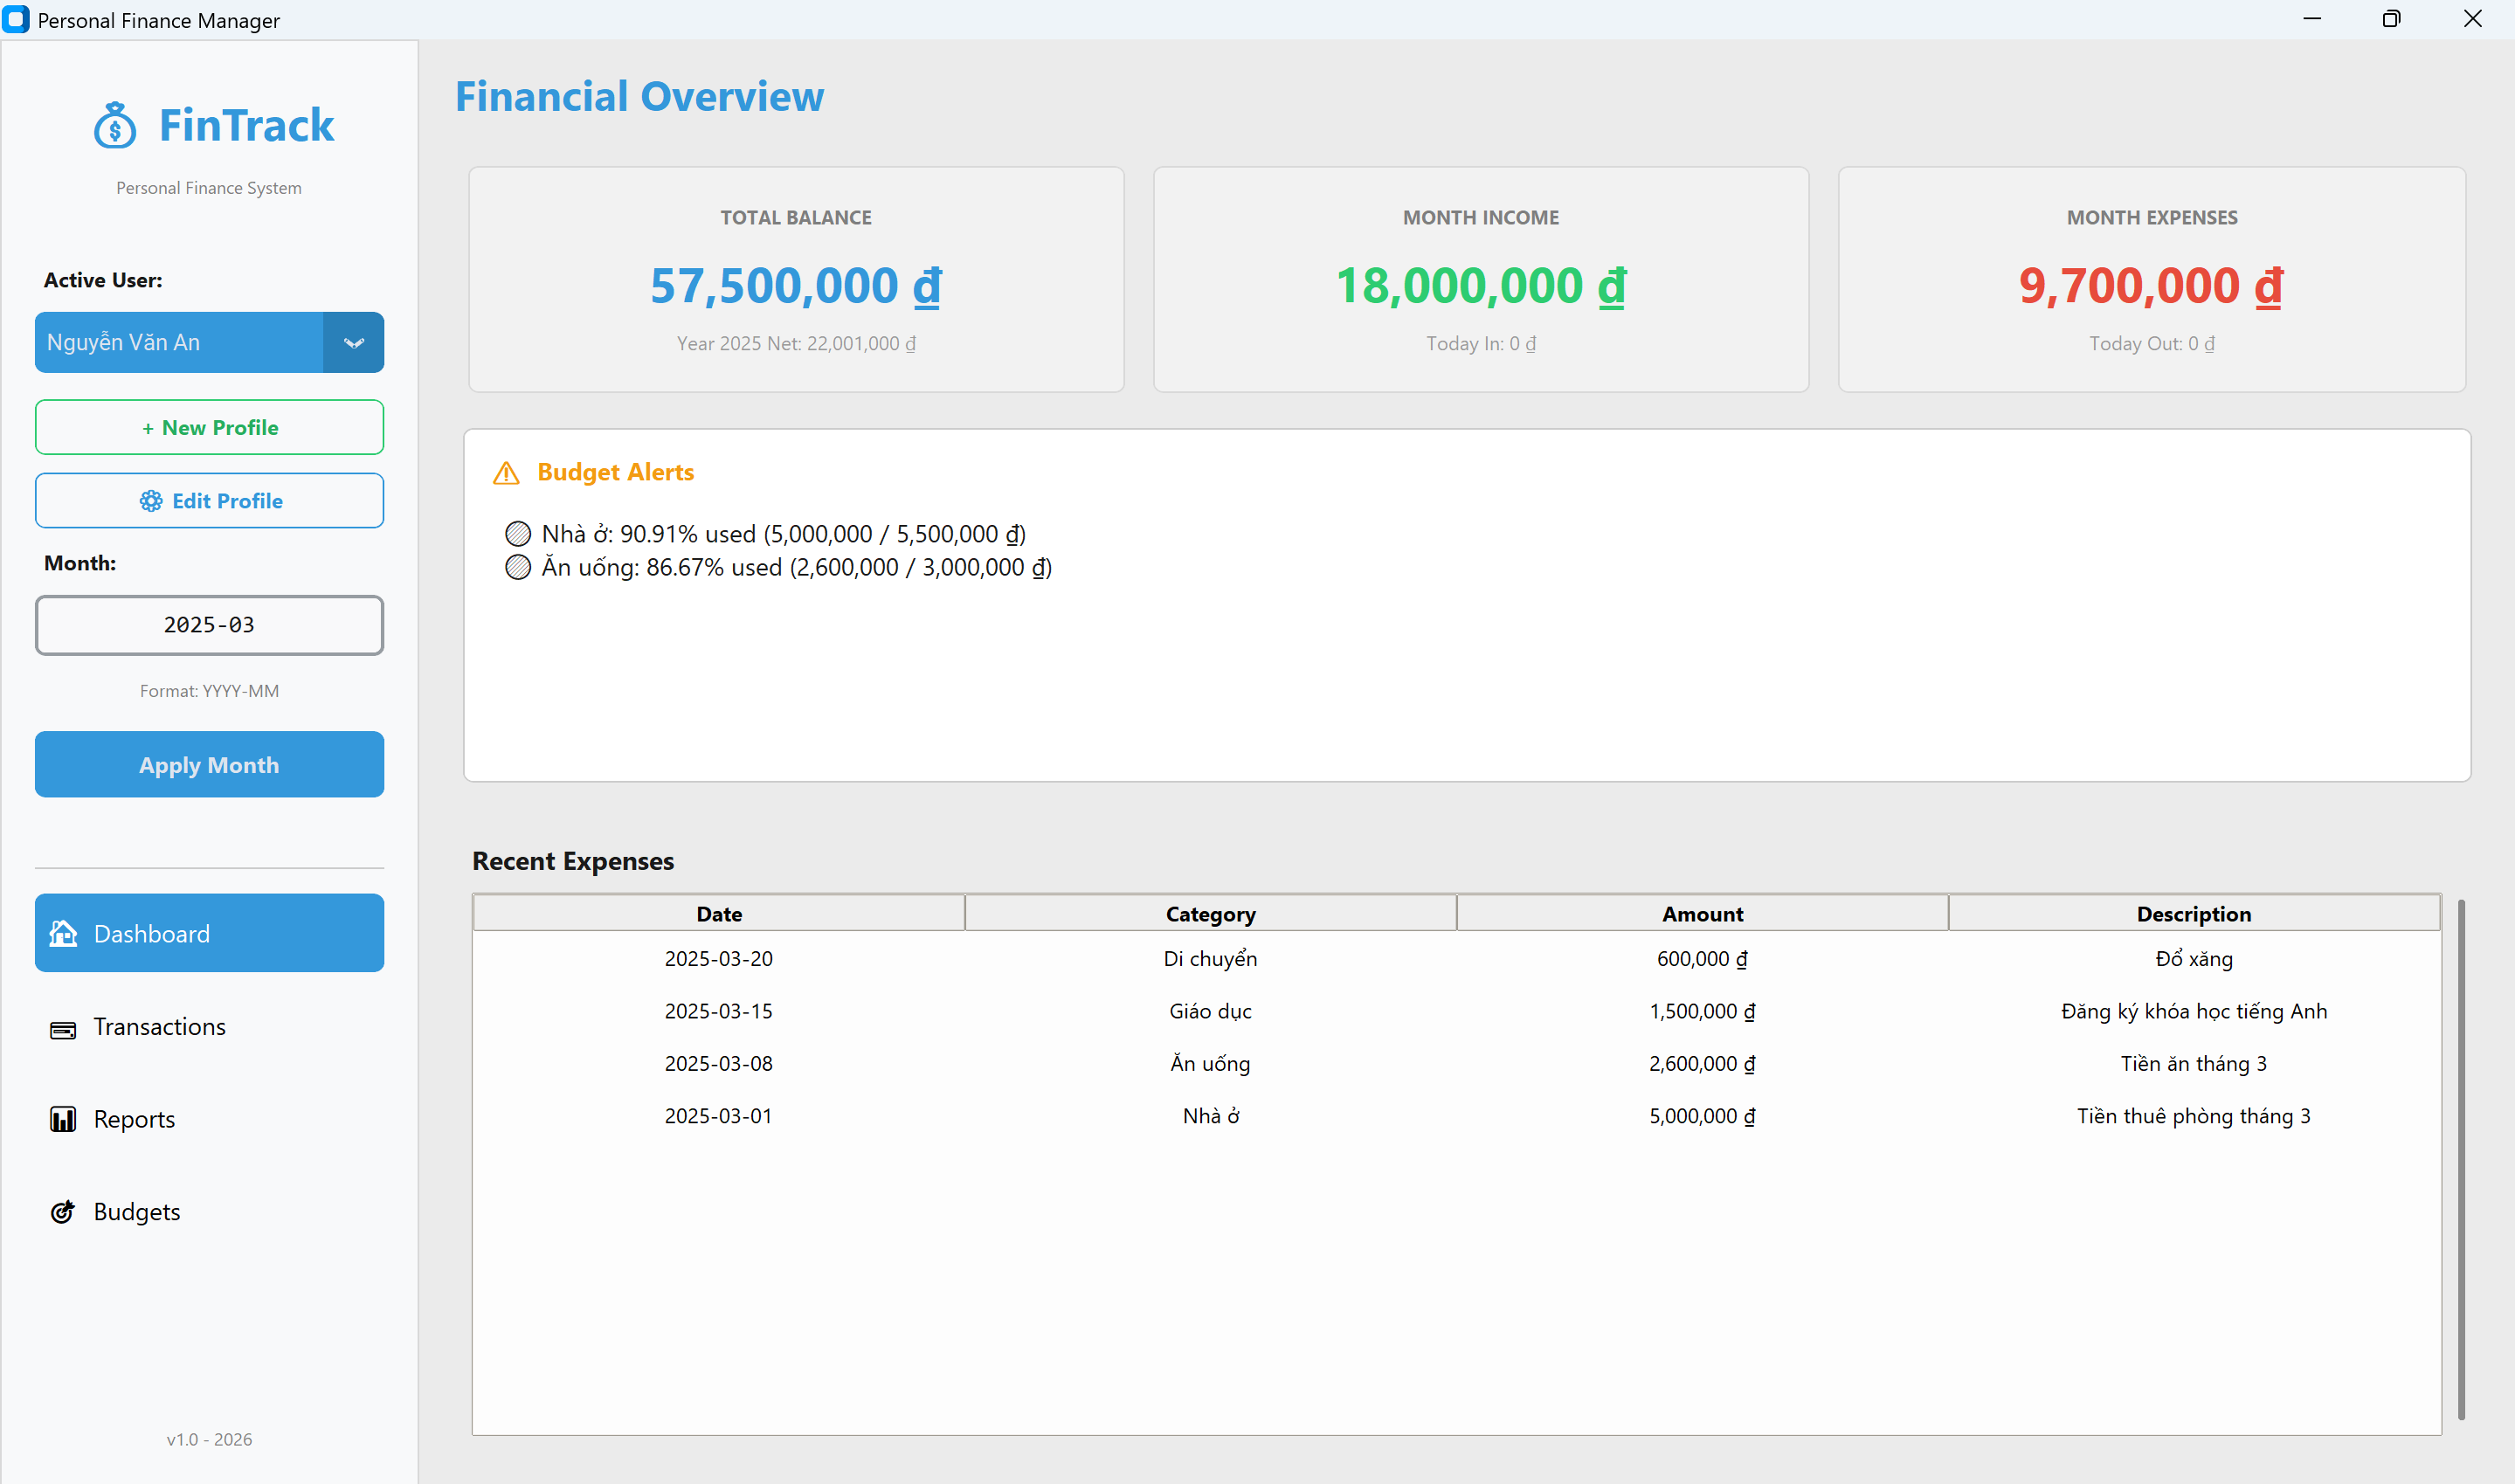
\includegraphics[width=0.92\textwidth]{screenshot/dashboard.png}
  \caption{Dashboard screen showing three KPI cards (Total Balance, Month Income,
           Month Expenses), each with a secondary sub-metric: yearly net savings
           (\emph{Year 2025 Net}), today's income (\emph{Today In}), and today's
           expenses (\emph{Today Out}). The Budget Alerts panel lists categories
           at WARNING or EXCEEDED status from \texttt{vw\_budget\_status}.
           The Recent Expenses table shows the latest transactions for the
           selected month. User: Nguyen Van An, Month: 2025-03.}
\end{figure}

The Dashboard queries four data sources on every \texttt{refresh()} call:
\begin{itemize}[leftmargin=2em]
  \item \texttt{get\_total\_balance(user\_id)} -- sums \texttt{BankAccounts.Balance}.
  \item \texttt{get\_yearly\_summary(user\_id, year)} -- yearly net displayed as a
        sub-label under Total Balance.
  \item \texttt{get\_daily\_summary(user\_id)} -- today's income and expense totals
        shown as sub-labels under Month Income and Month Expenses.
  \item \texttt{get\_budget\_alerts(user\_id, month\_year)} -- queries
        \texttt{vw\_budget\_status} for WARNING and EXCEEDED rows only.
\end{itemize}

\subsubsection{Transactions -- Add Income}

\begin{figure}[H]
  \centering
  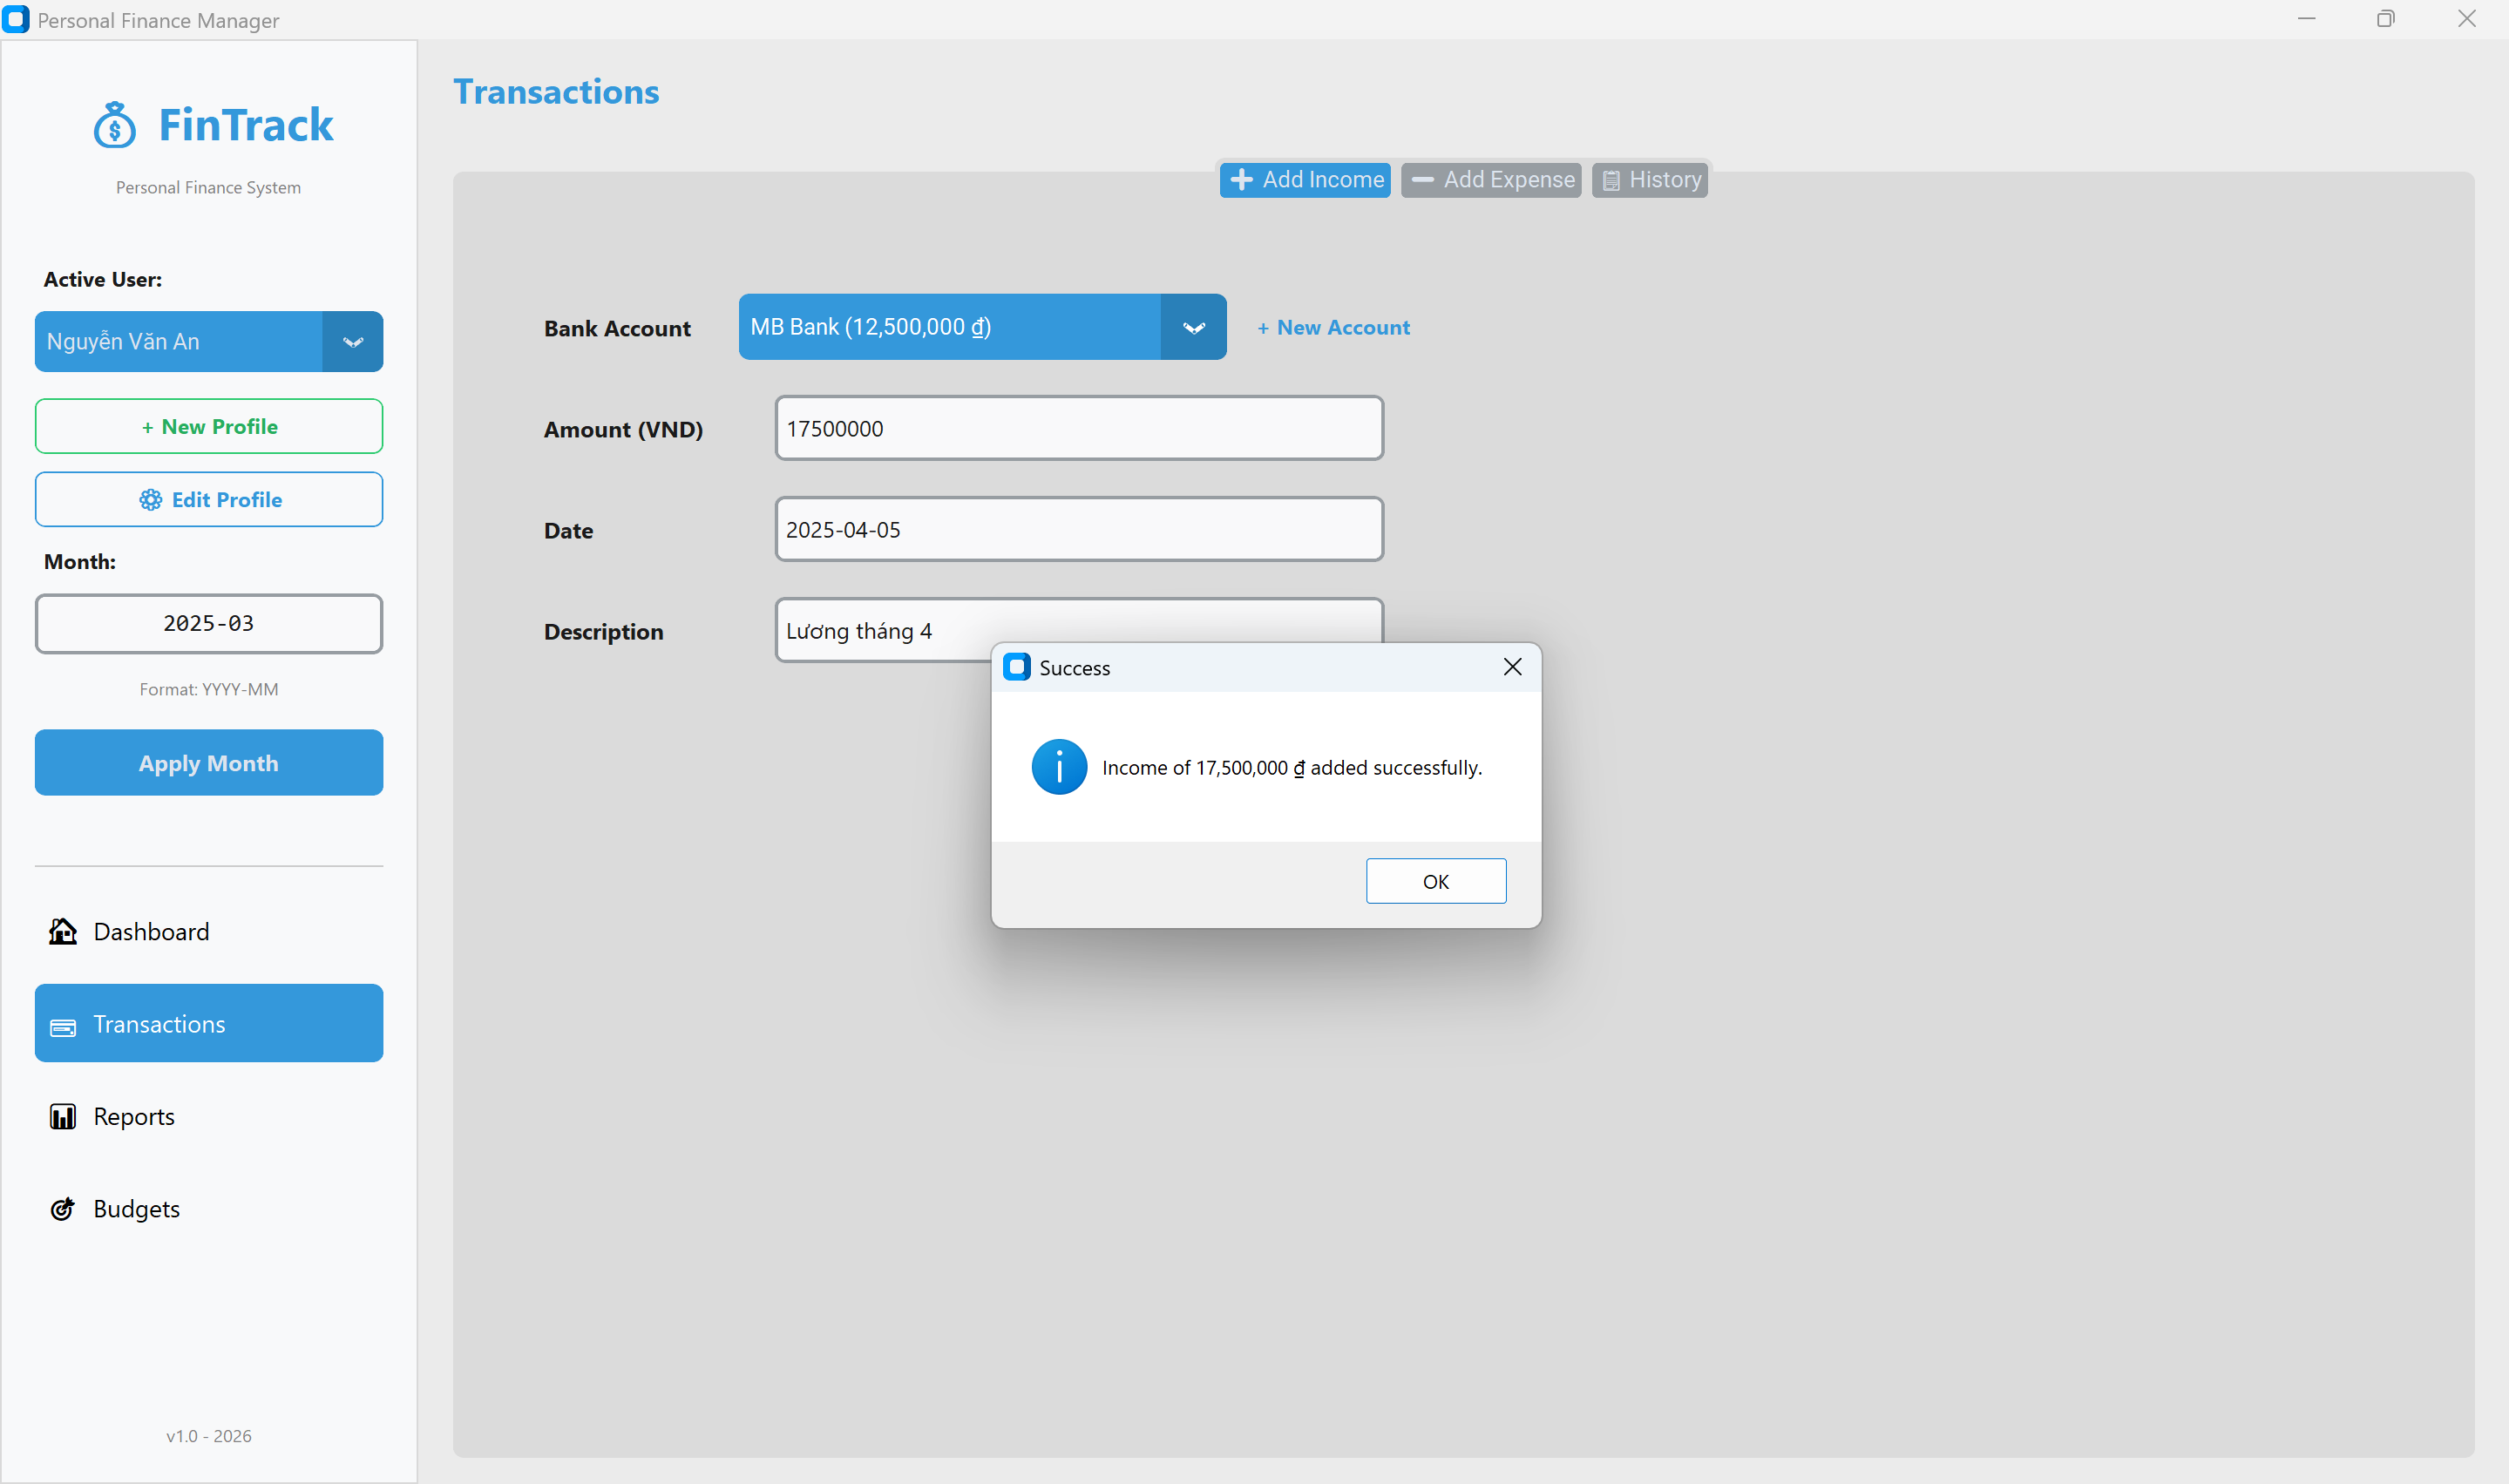
\includegraphics[width=0.85\textwidth]{screenshot/add_income.png}
  \caption{Add Income tab: user enters 17,500,000 VND into MB Bank for 2025-04-05.
           The success dialog confirms the record was saved and the bank balance
           was incremented automatically by \texttt{trg\_income\_after\_insert}.
           The Transactions screen provides three tabs: Add Income, Add Expense,
           and History.}
\end{figure}

\subsubsection{Transactions -- Add Expense and Add New Category}

\begin{figure}[H]
  \centering
  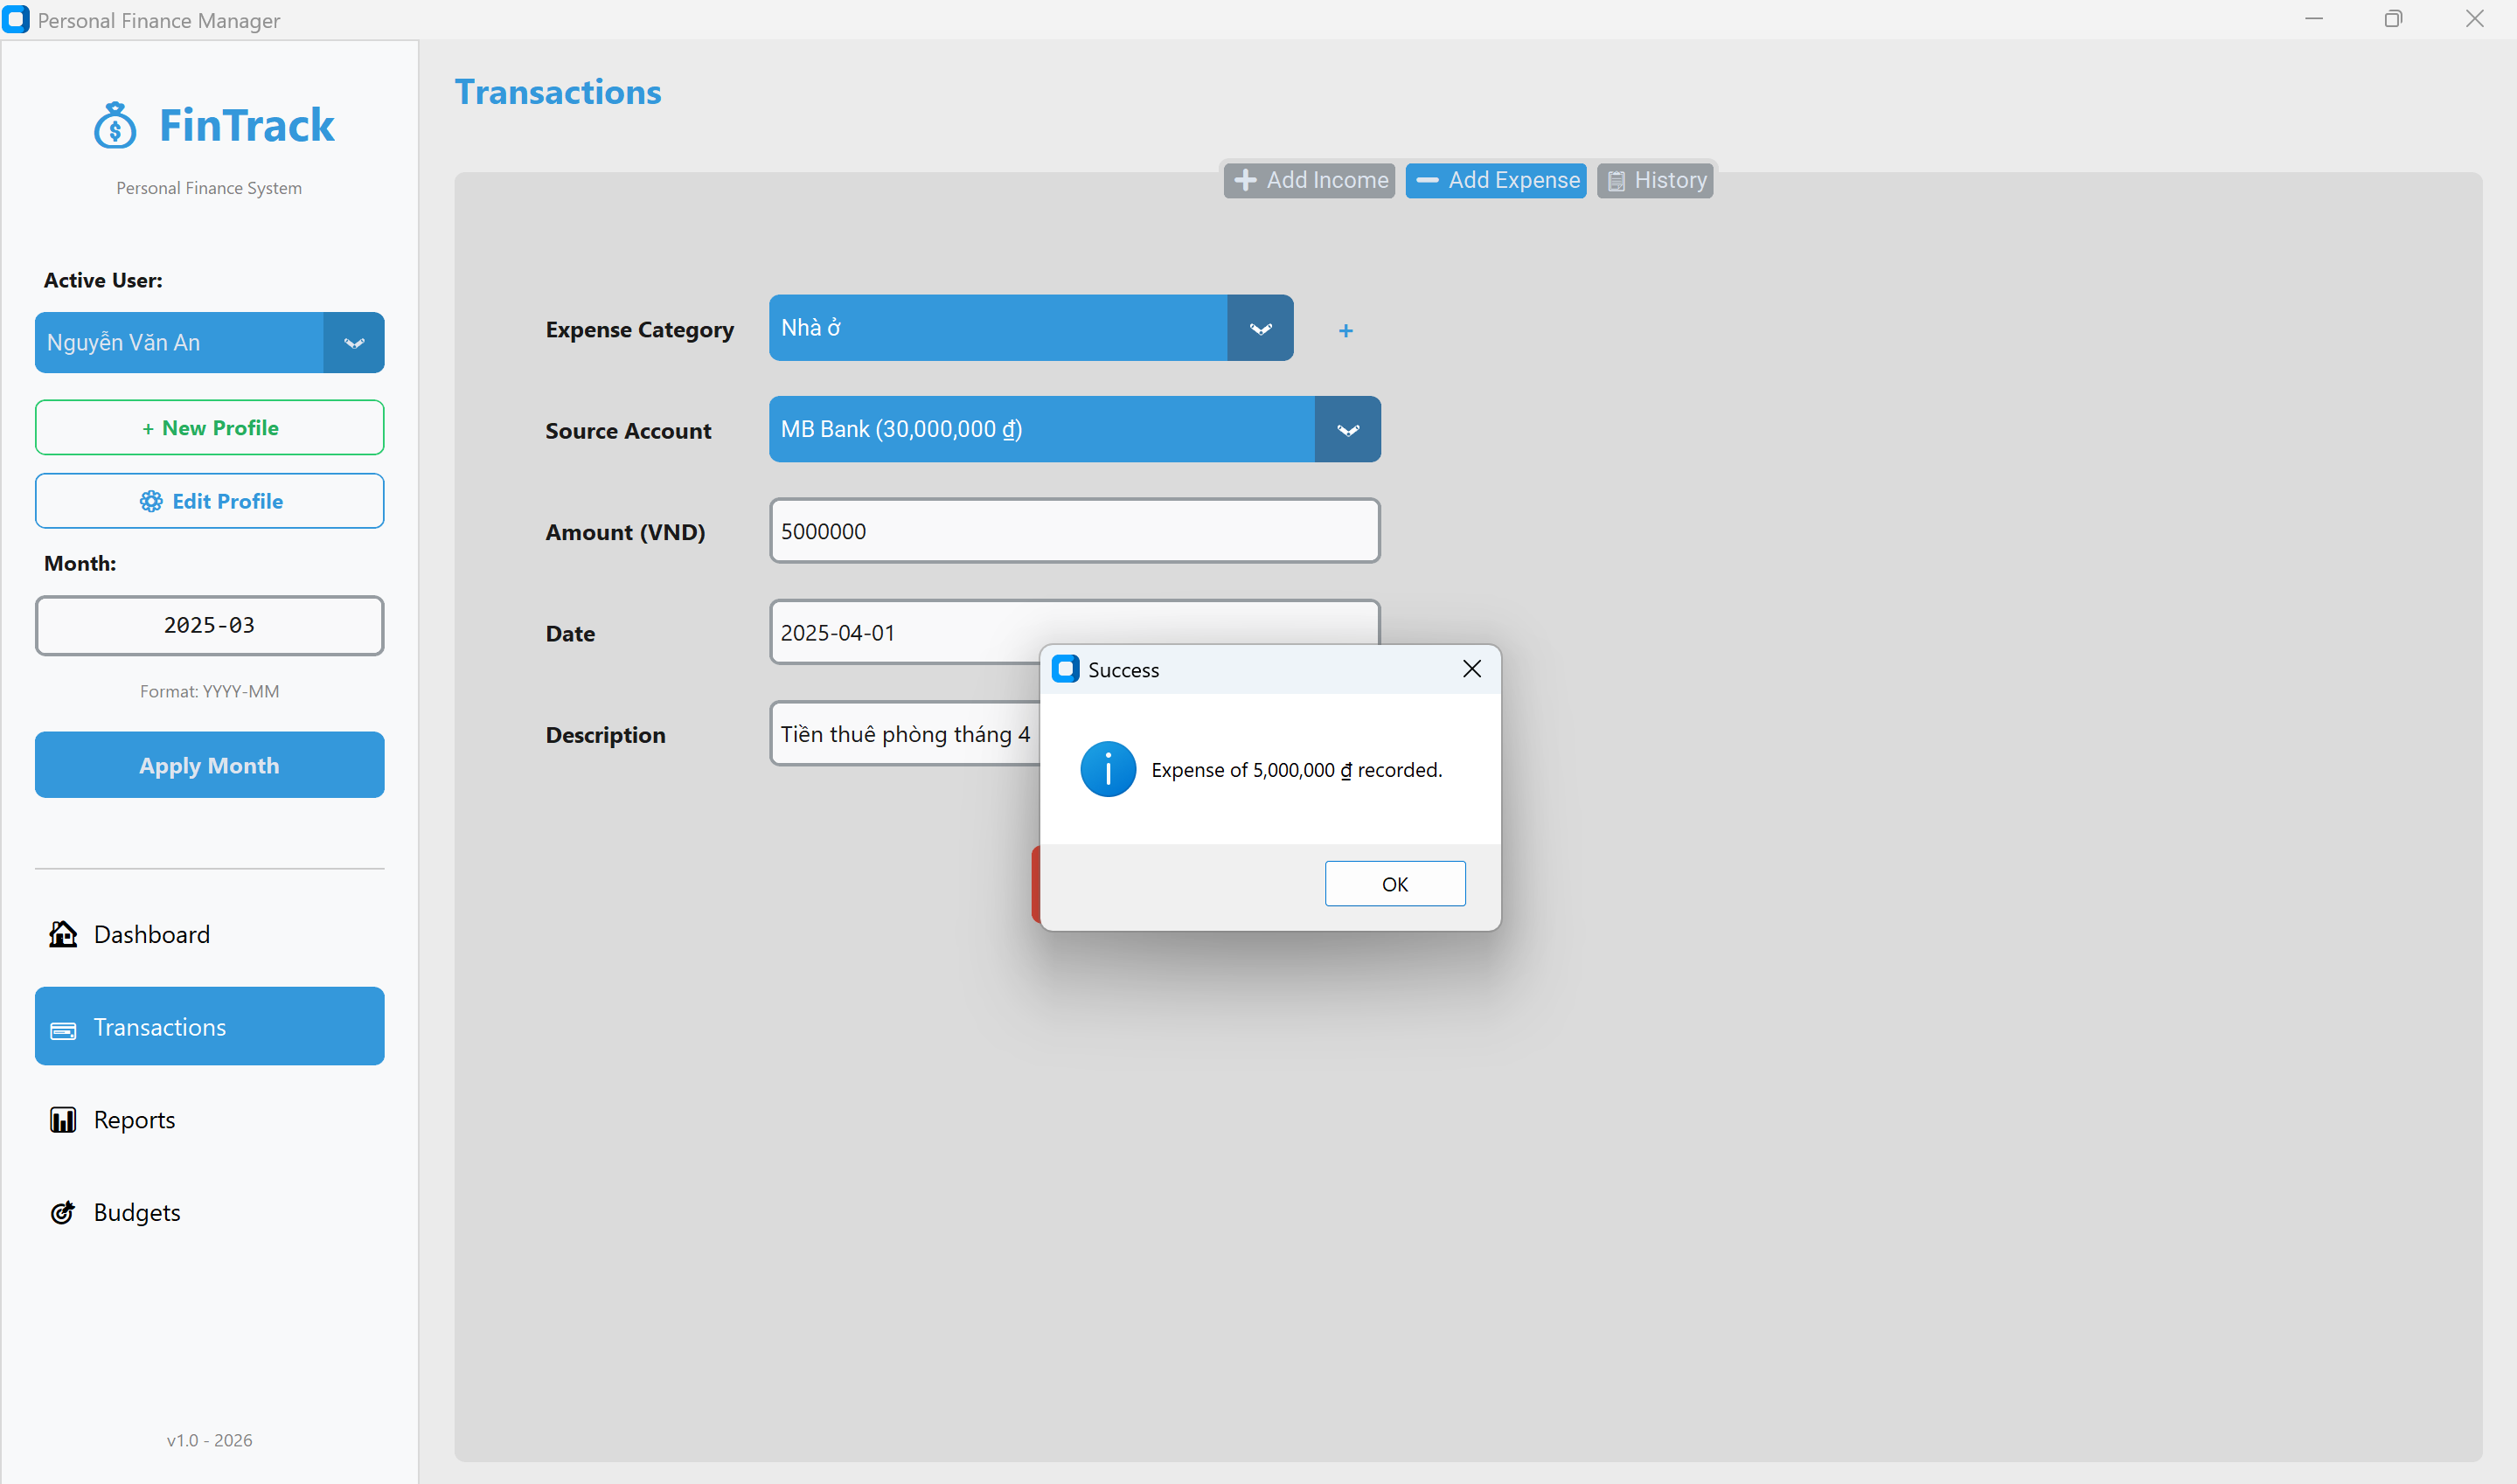
\includegraphics[width=0.85\textwidth]{screenshot/add_expense.png}
  \caption{Add Expense tab: user records a 5,000,000 VND housing expense
           (Nha o) debited from MB Bank. The trigger
           \texttt{trg\_expense\_after\_insert} immediately decremented the
           account balance upon commit.}
\end{figure}

\begin{figure}[H]
  \centering
  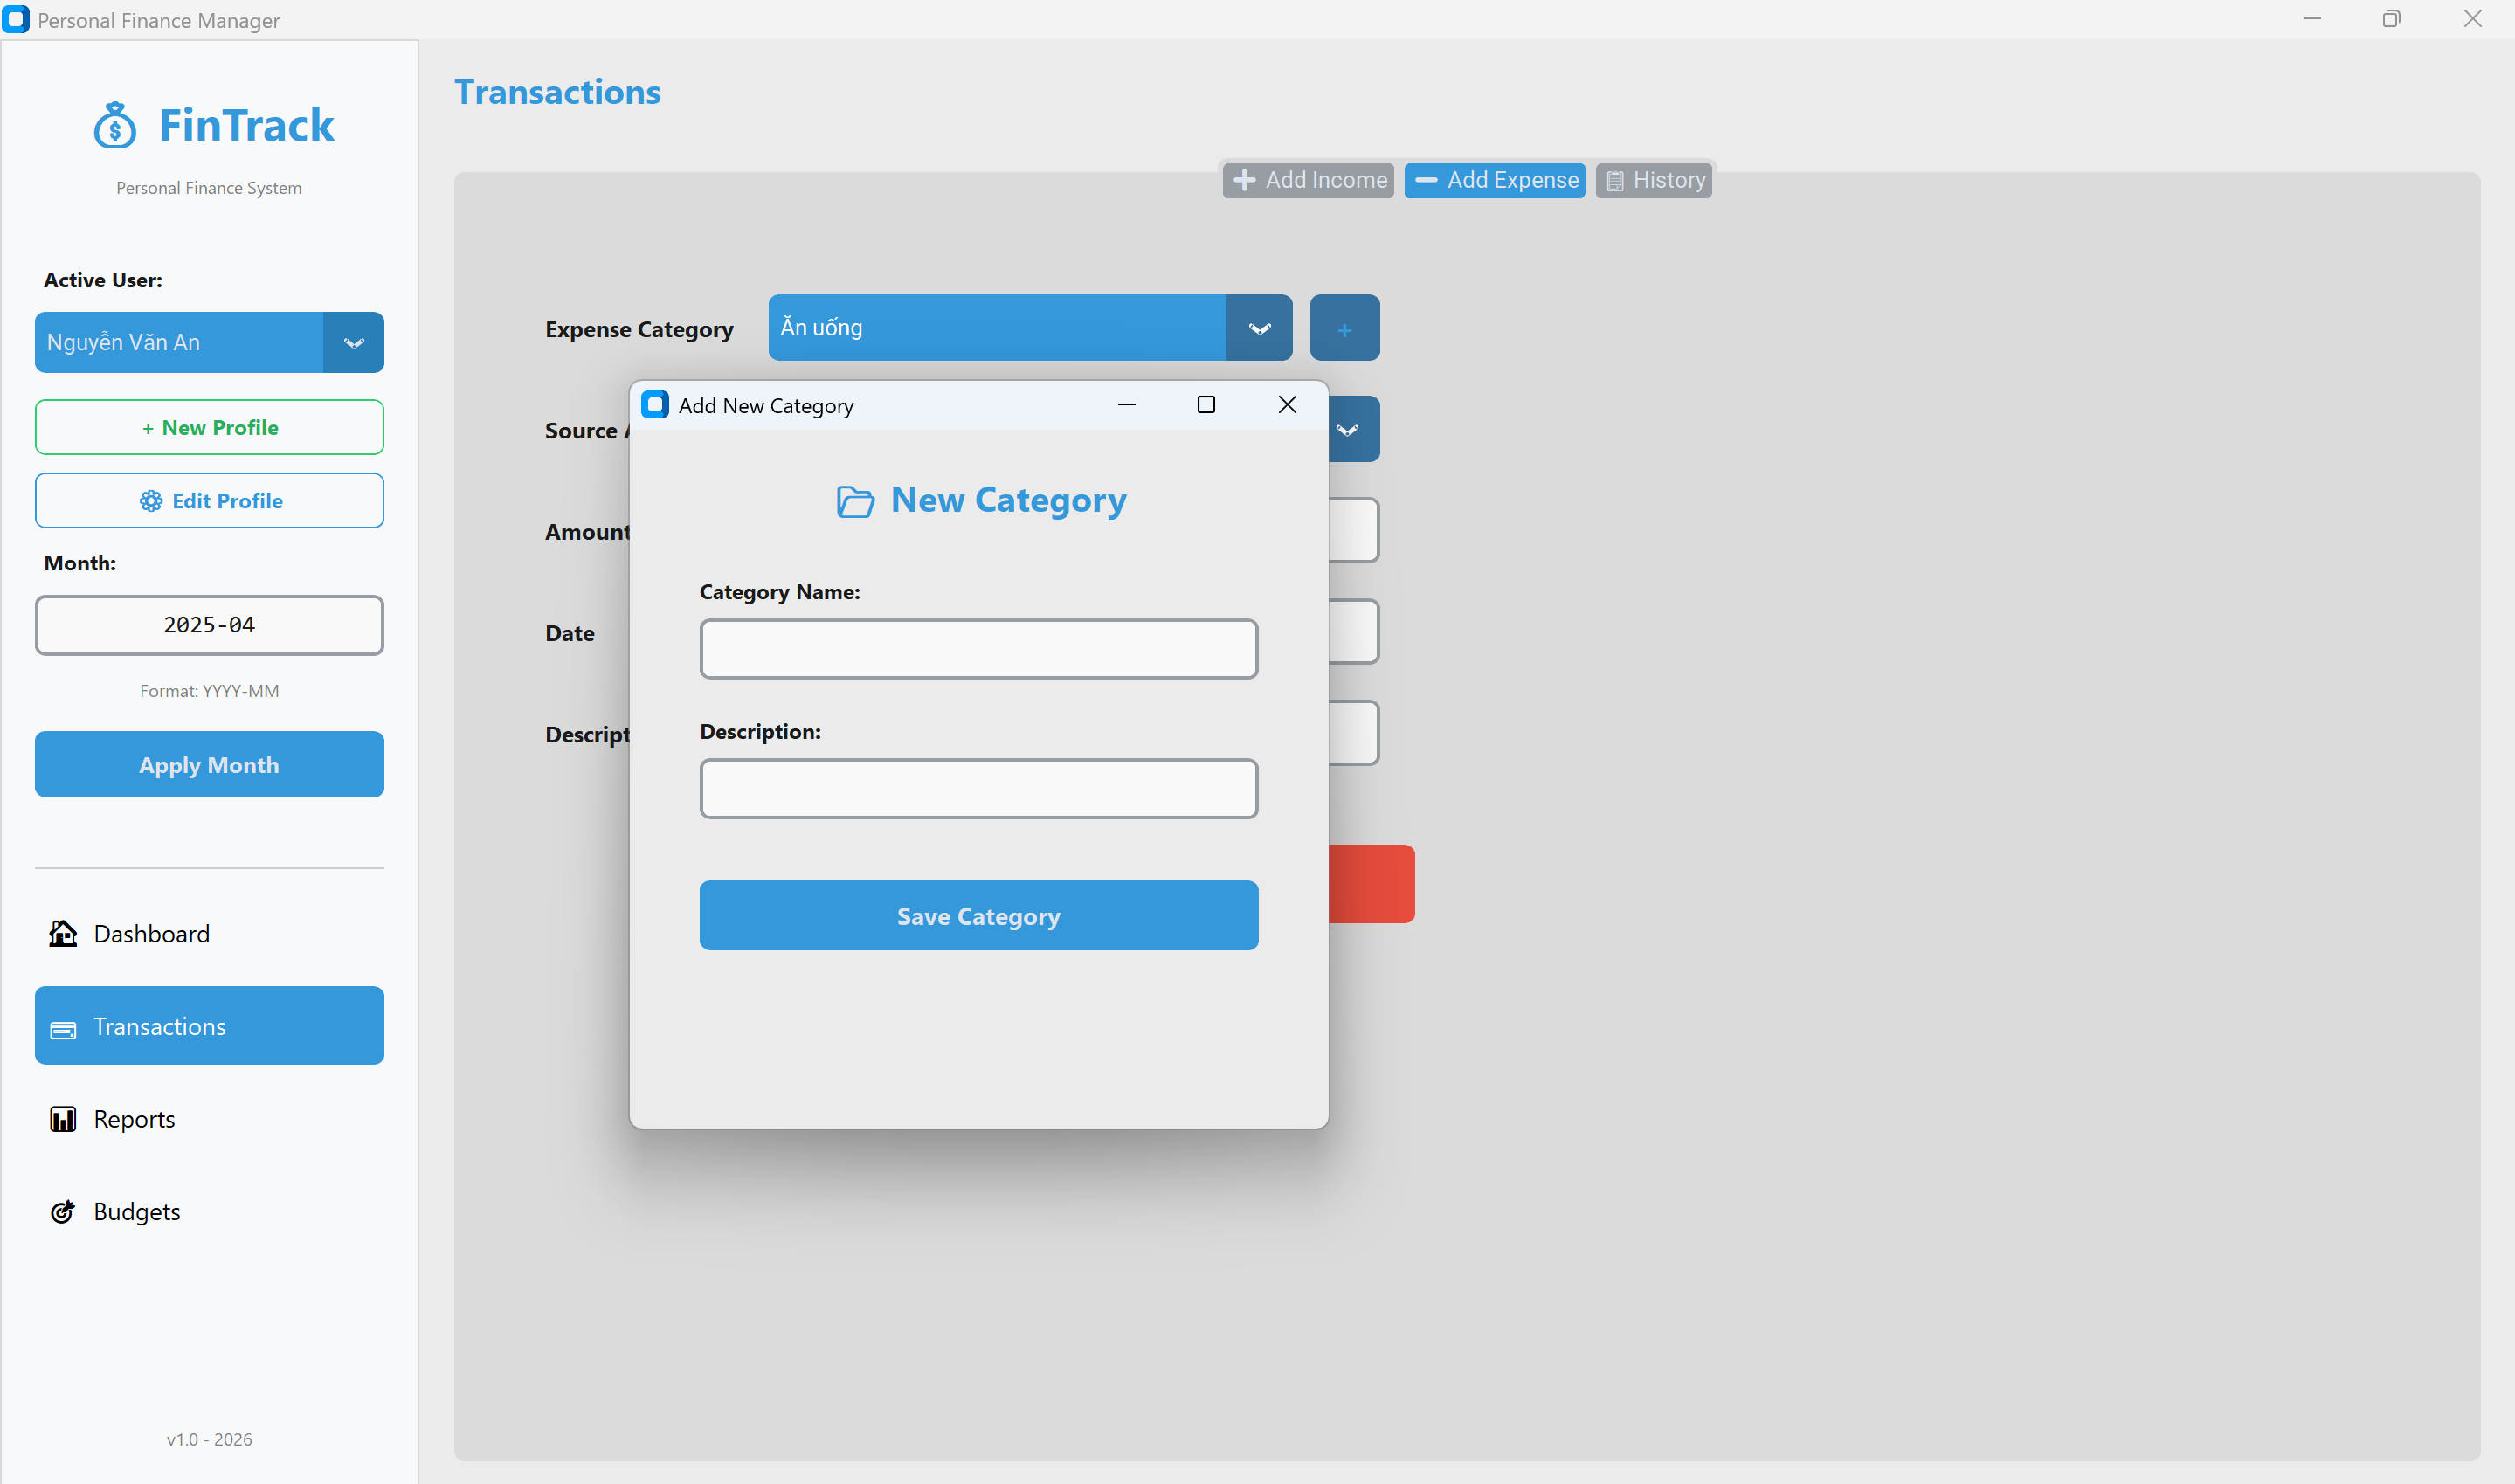
\includegraphics[width=0.75\textwidth]{screenshot/add_category.png}
  \caption{Add New Category dialog, opened from the \texttt{+} button beside
           the Expense Category dropdown. The user enters a Category Name and
           optional Description. Clicking Save Category calls
           \texttt{create\_category()}, which inserts a row into
           \texttt{ExpenseCategories} and returns the new \texttt{CategoryID}.
           The parent dropdown refreshes immediately to include the new entry.}
\end{figure}

\subsubsection{Transactions -- History, Edit, and Delete}

\begin{figure}[H]
  \centering
  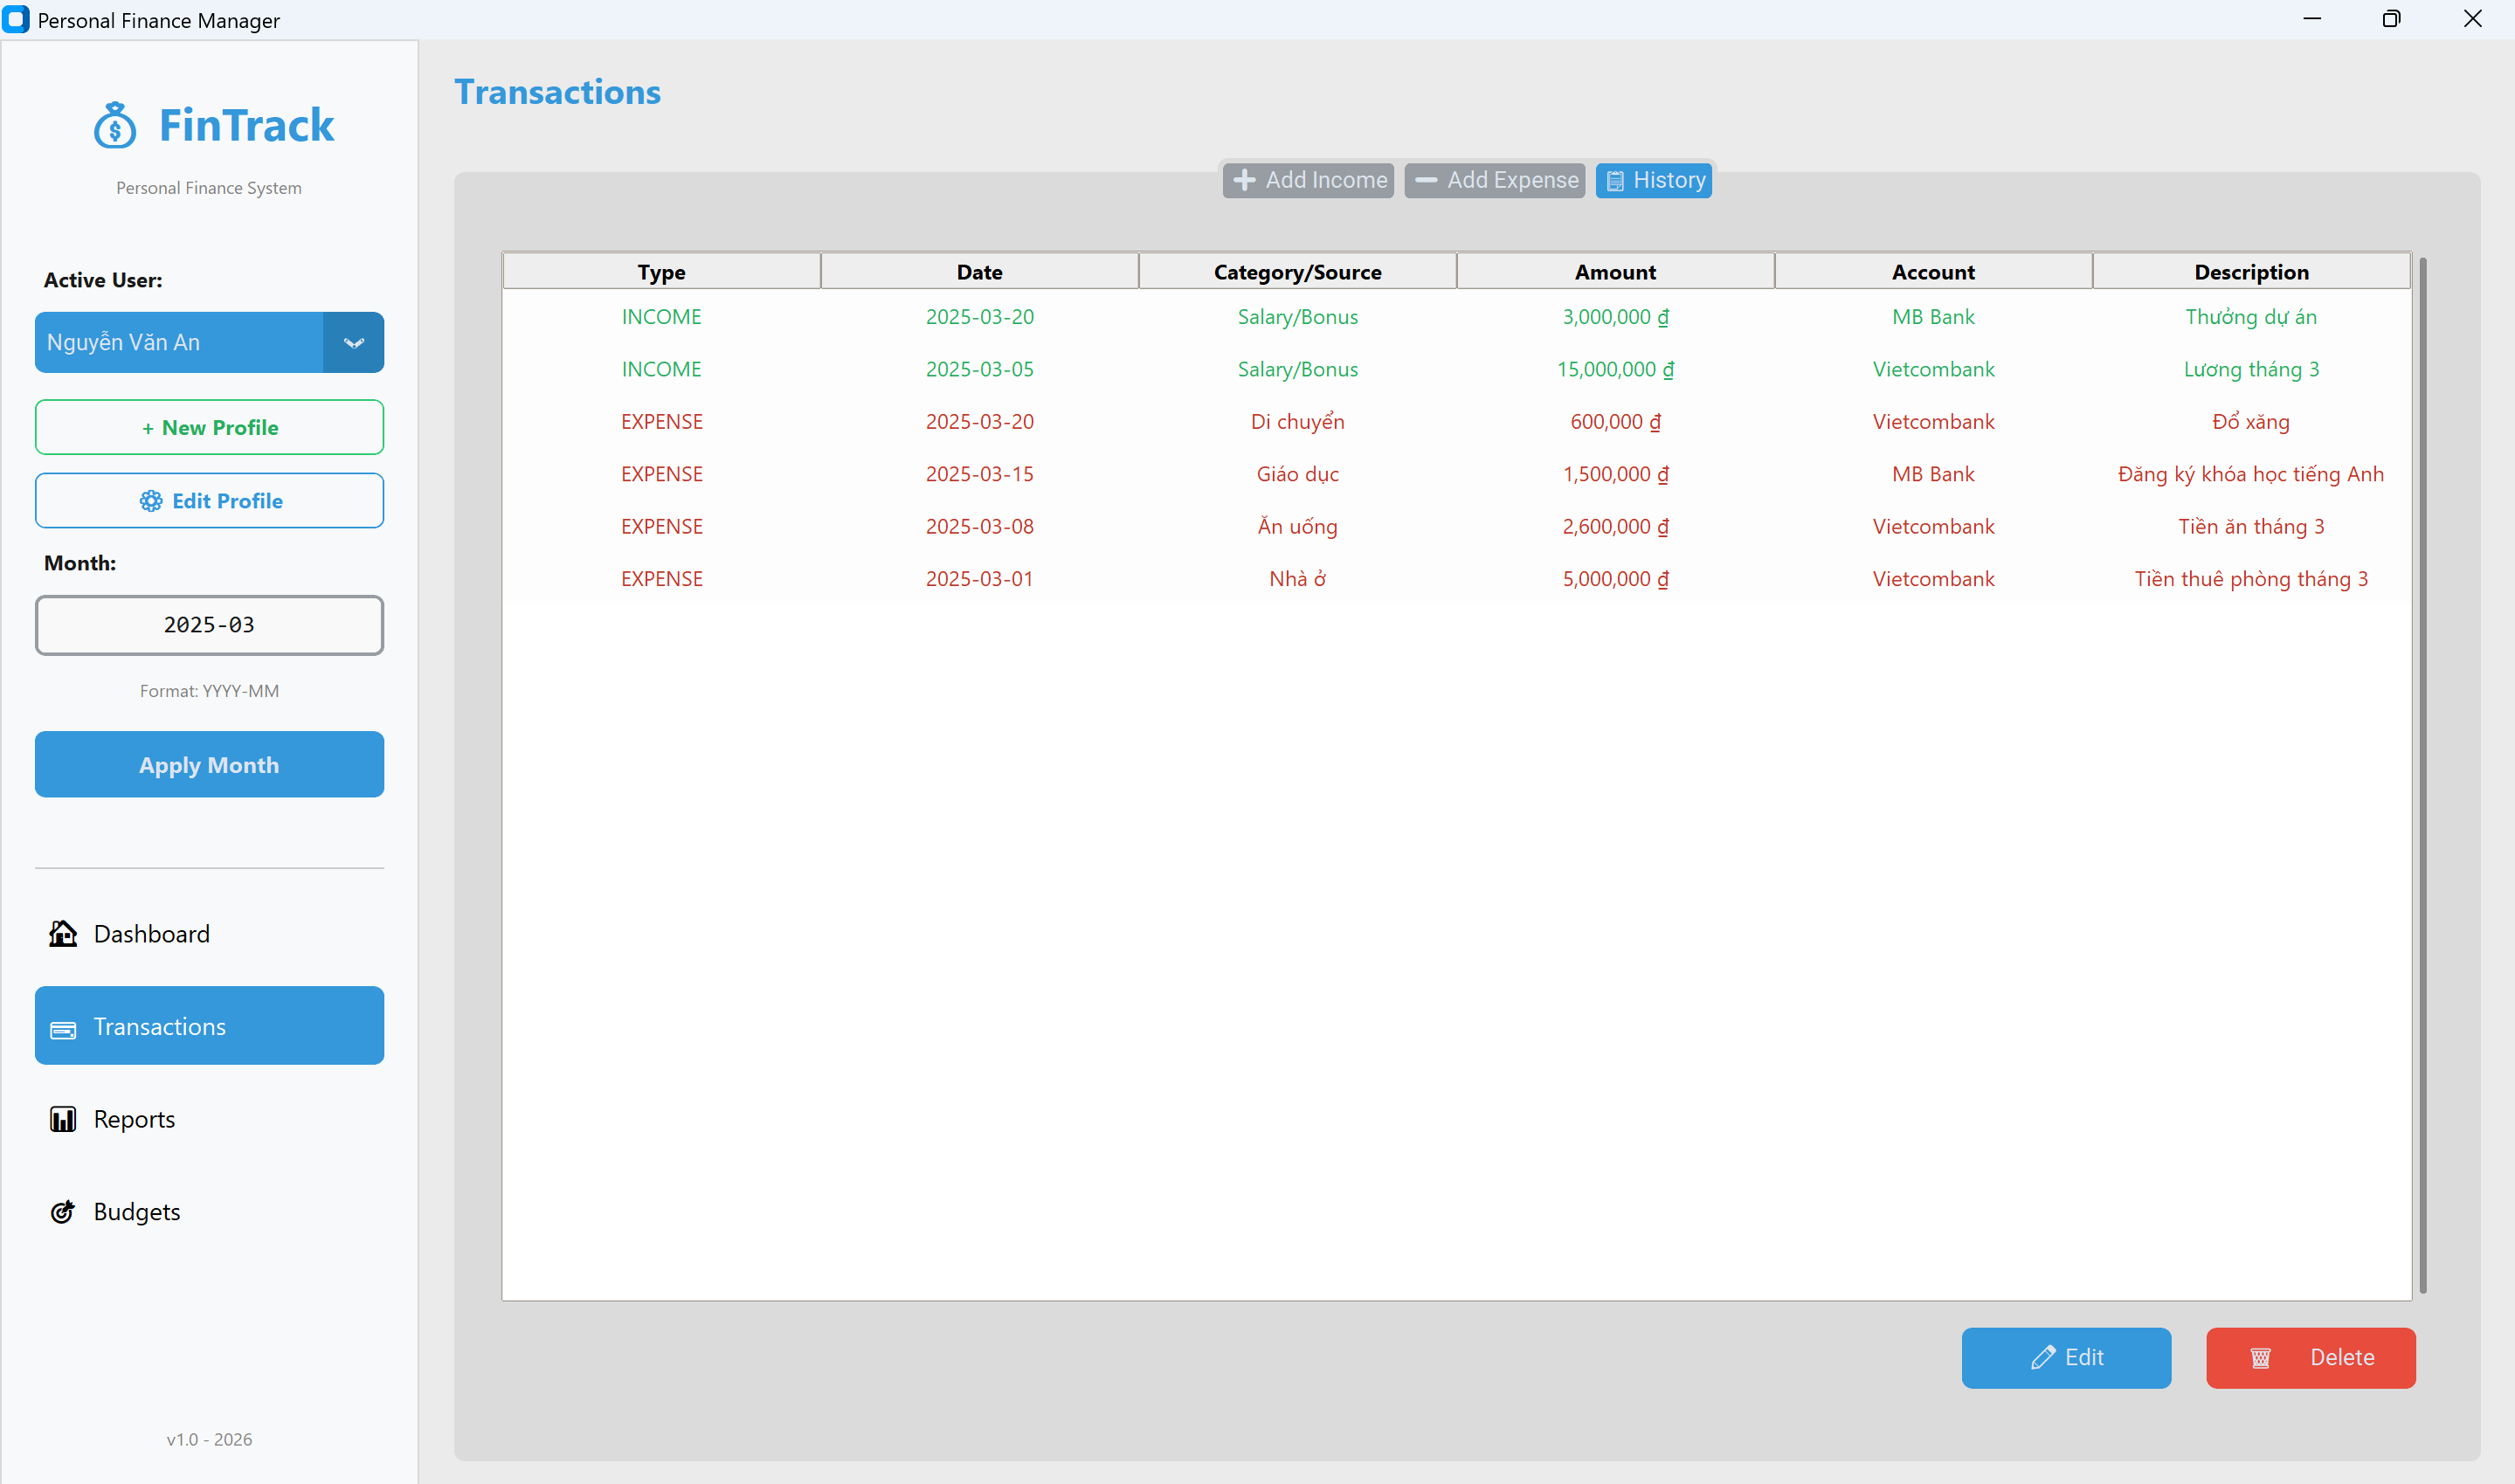
\includegraphics[width=0.92\textwidth]{screenshot/history.png}
  \caption{History tab showing all income (green) and expense (red) records
           for the selected month in a unified table. Columns include Type,
           Date, Category/Source, Amount, Account, and Description. Selecting
           a row enables the Edit and Delete buttons at the bottom right.}
\end{figure}

\begin{figure}[H]
  \centering
  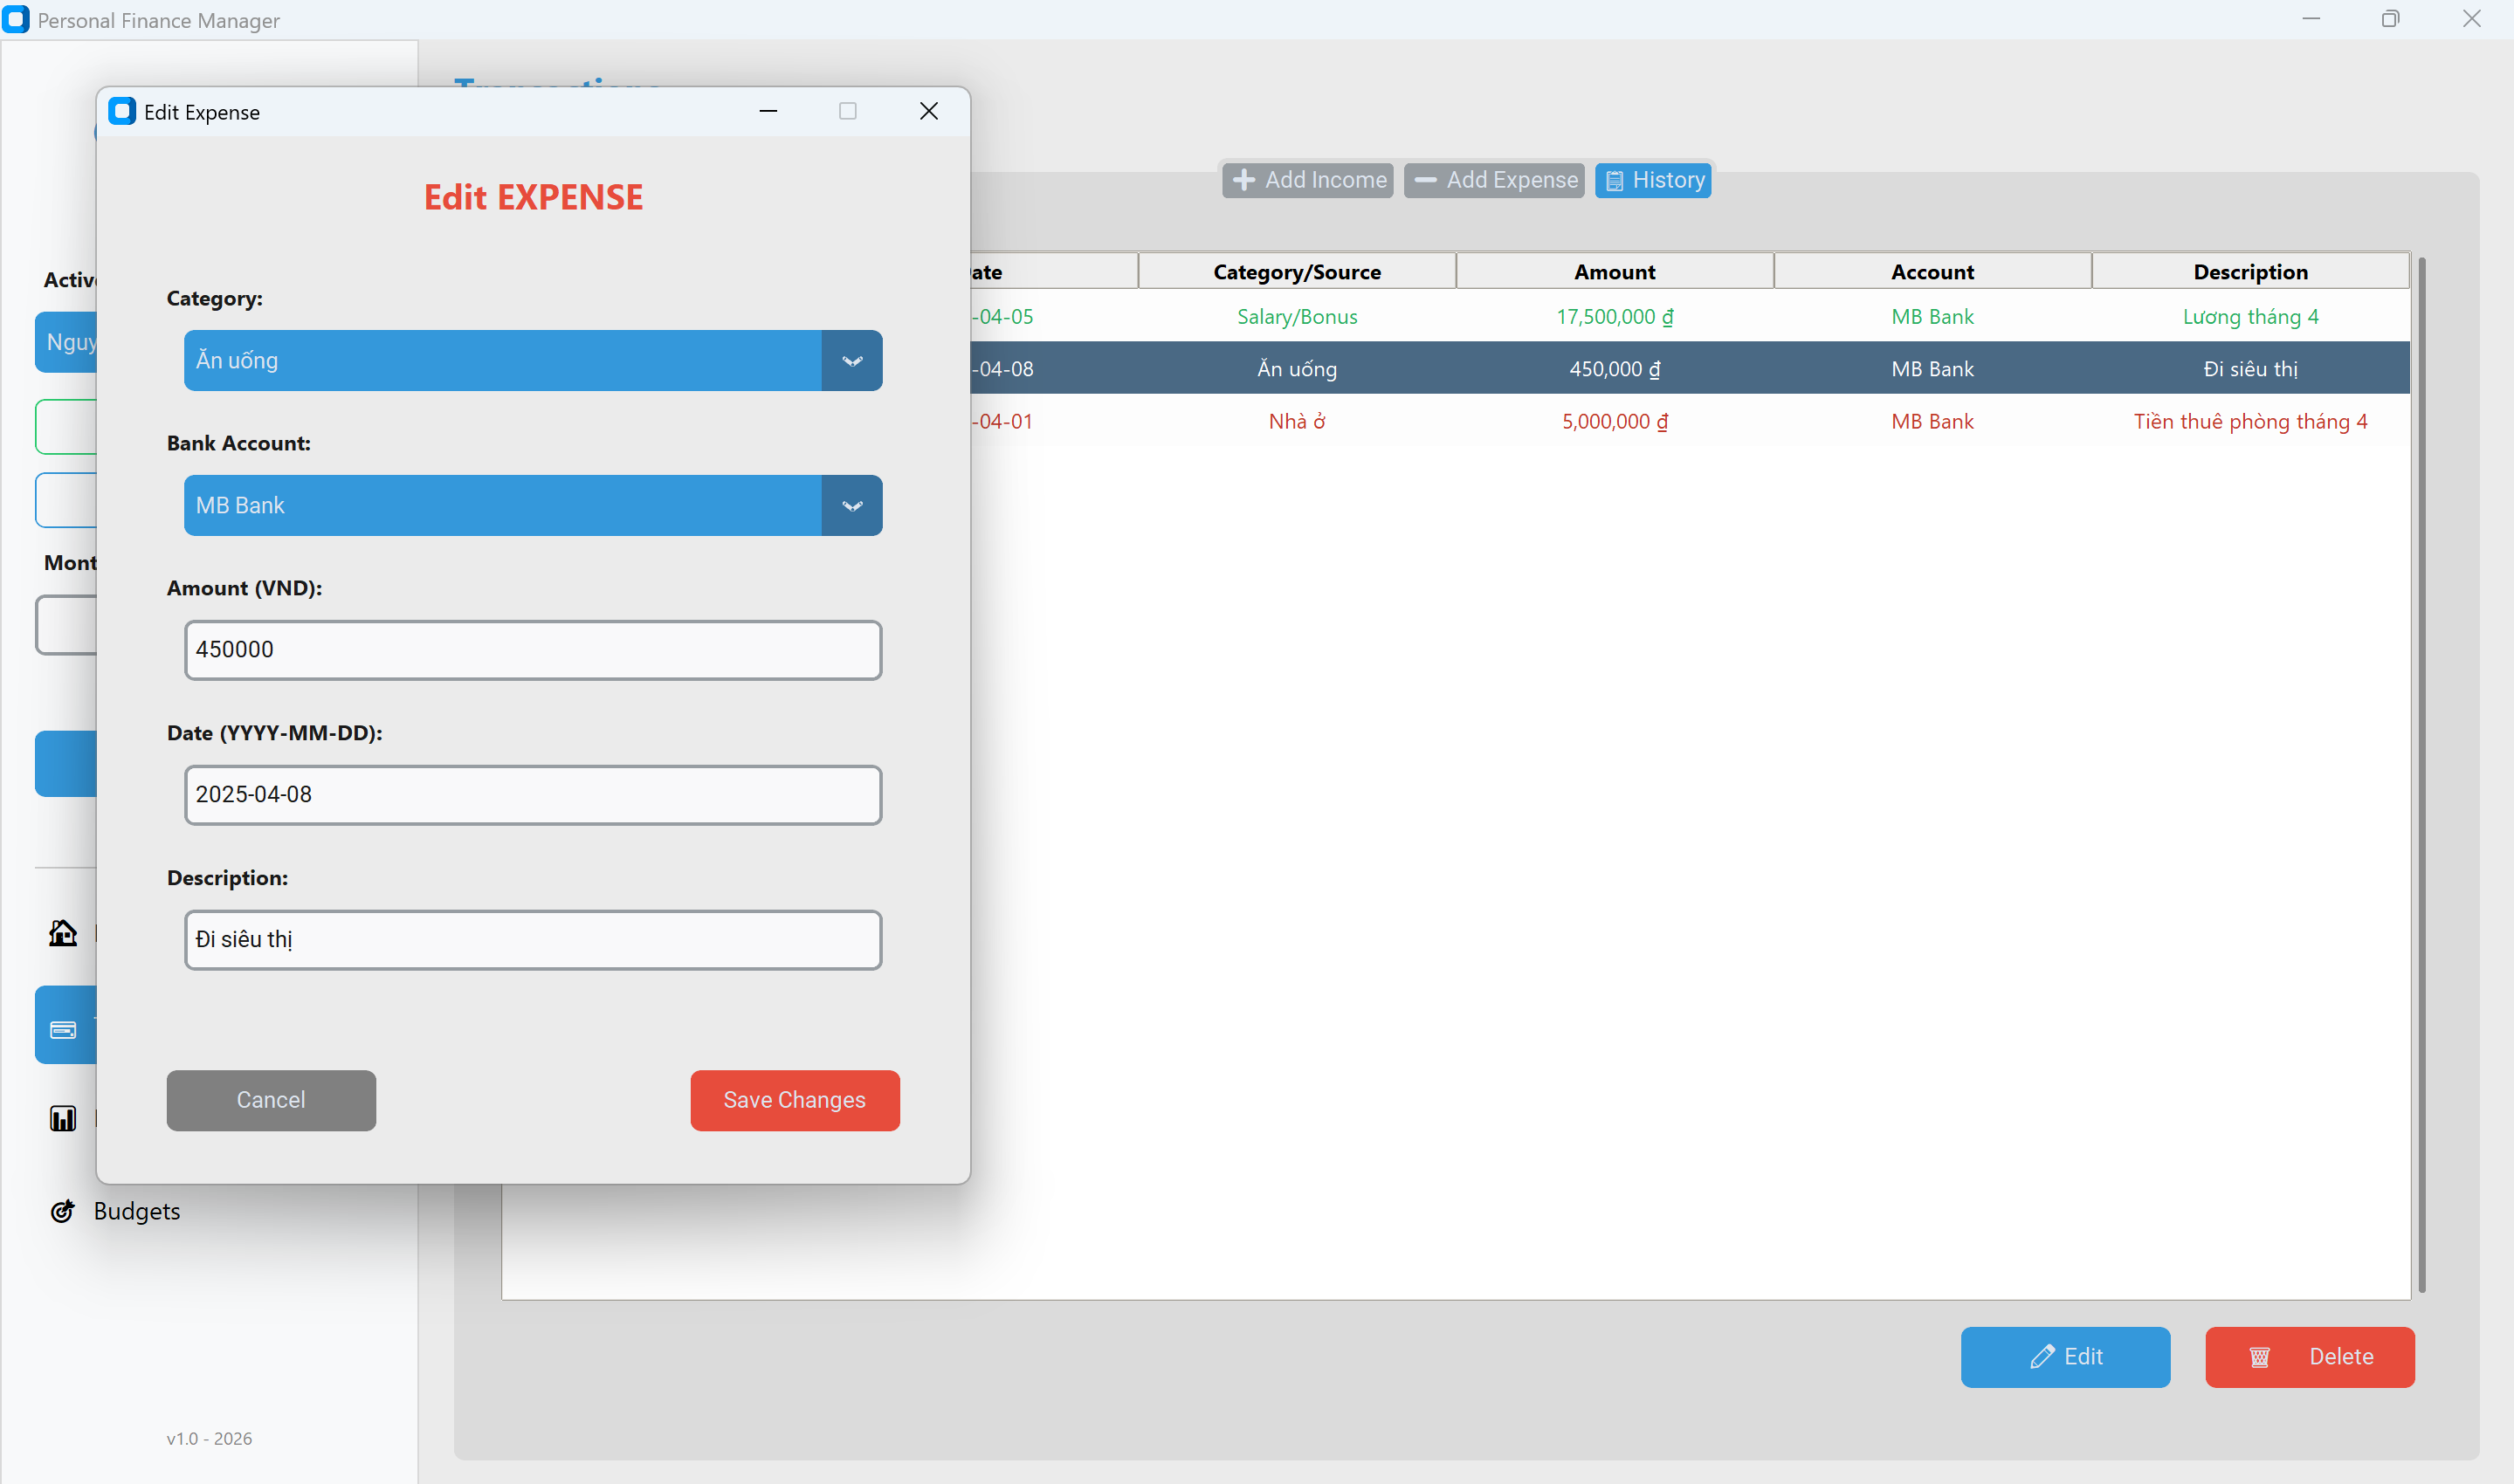
\includegraphics[width=0.75\textwidth]{screenshot/edit_expense.png}
  \caption{Edit Expense dialog, opened by selecting a row in the History tab.
           All fields are pre-populated with the existing record's values.
           Clicking Save Changes calls \texttt{update\_expense()}; the trigger
           \texttt{trg\_expense\_after\_update} automatically adjusts the account
           balance -- applying only the delta if the amount changed on the same
           account, or transferring between accounts if the Bank Account field
           was changed. The same modal pattern applies to income records via
           \texttt{update\_income()} and \texttt{trg\_income\_after\_update}.}
\end{figure}

\subsubsection{User Profile -- New Profile and Edit Profile}

\begin{figure}[H]
  \centering
  \begin{subfigure}[t]{0.48\textwidth}
    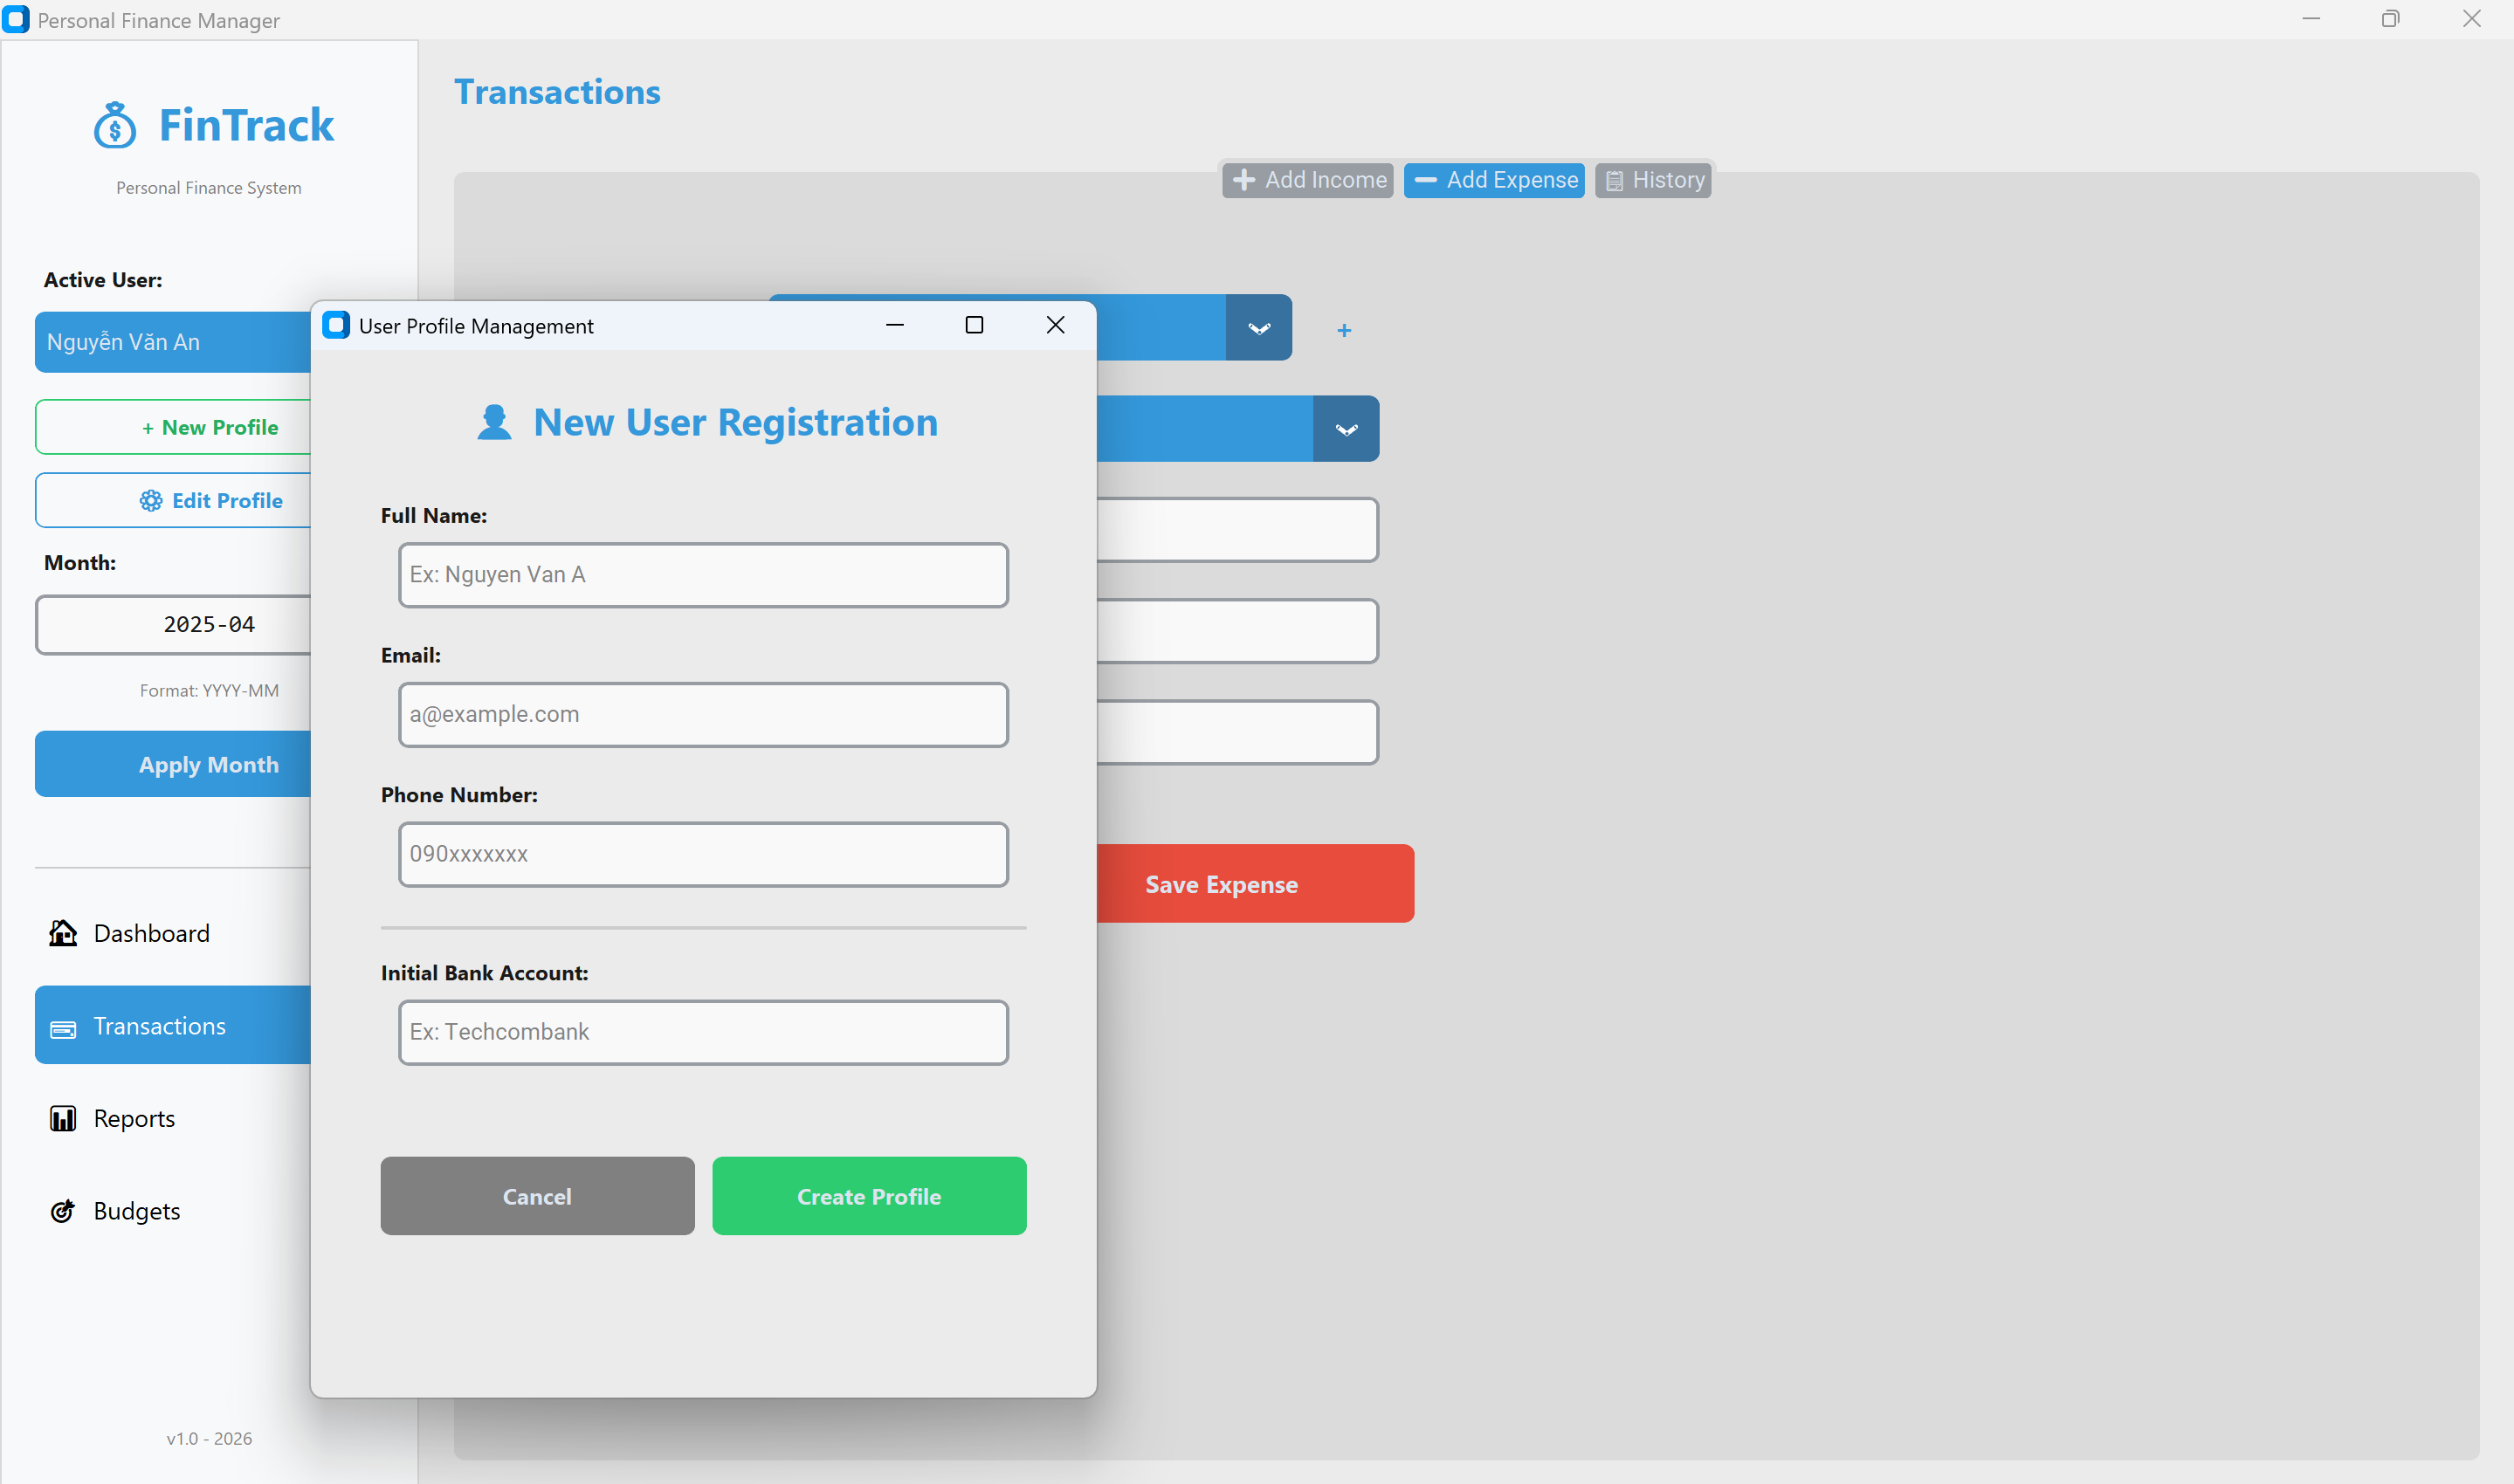
\includegraphics[width=\textwidth]{screenshot/new_profile.png}
    \caption{New User Registration dialog. Collects Full Name, Email,
             Phone Number, and Initial Bank Account name. Clicking
             Create Profile calls \texttt{create\_user()} followed by
             \texttt{create\_account()} to register the user and their
             first bank account in sequence.}
  \end{subfigure}
  \hfill
  \begin{subfigure}[t]{0.48\textwidth}
    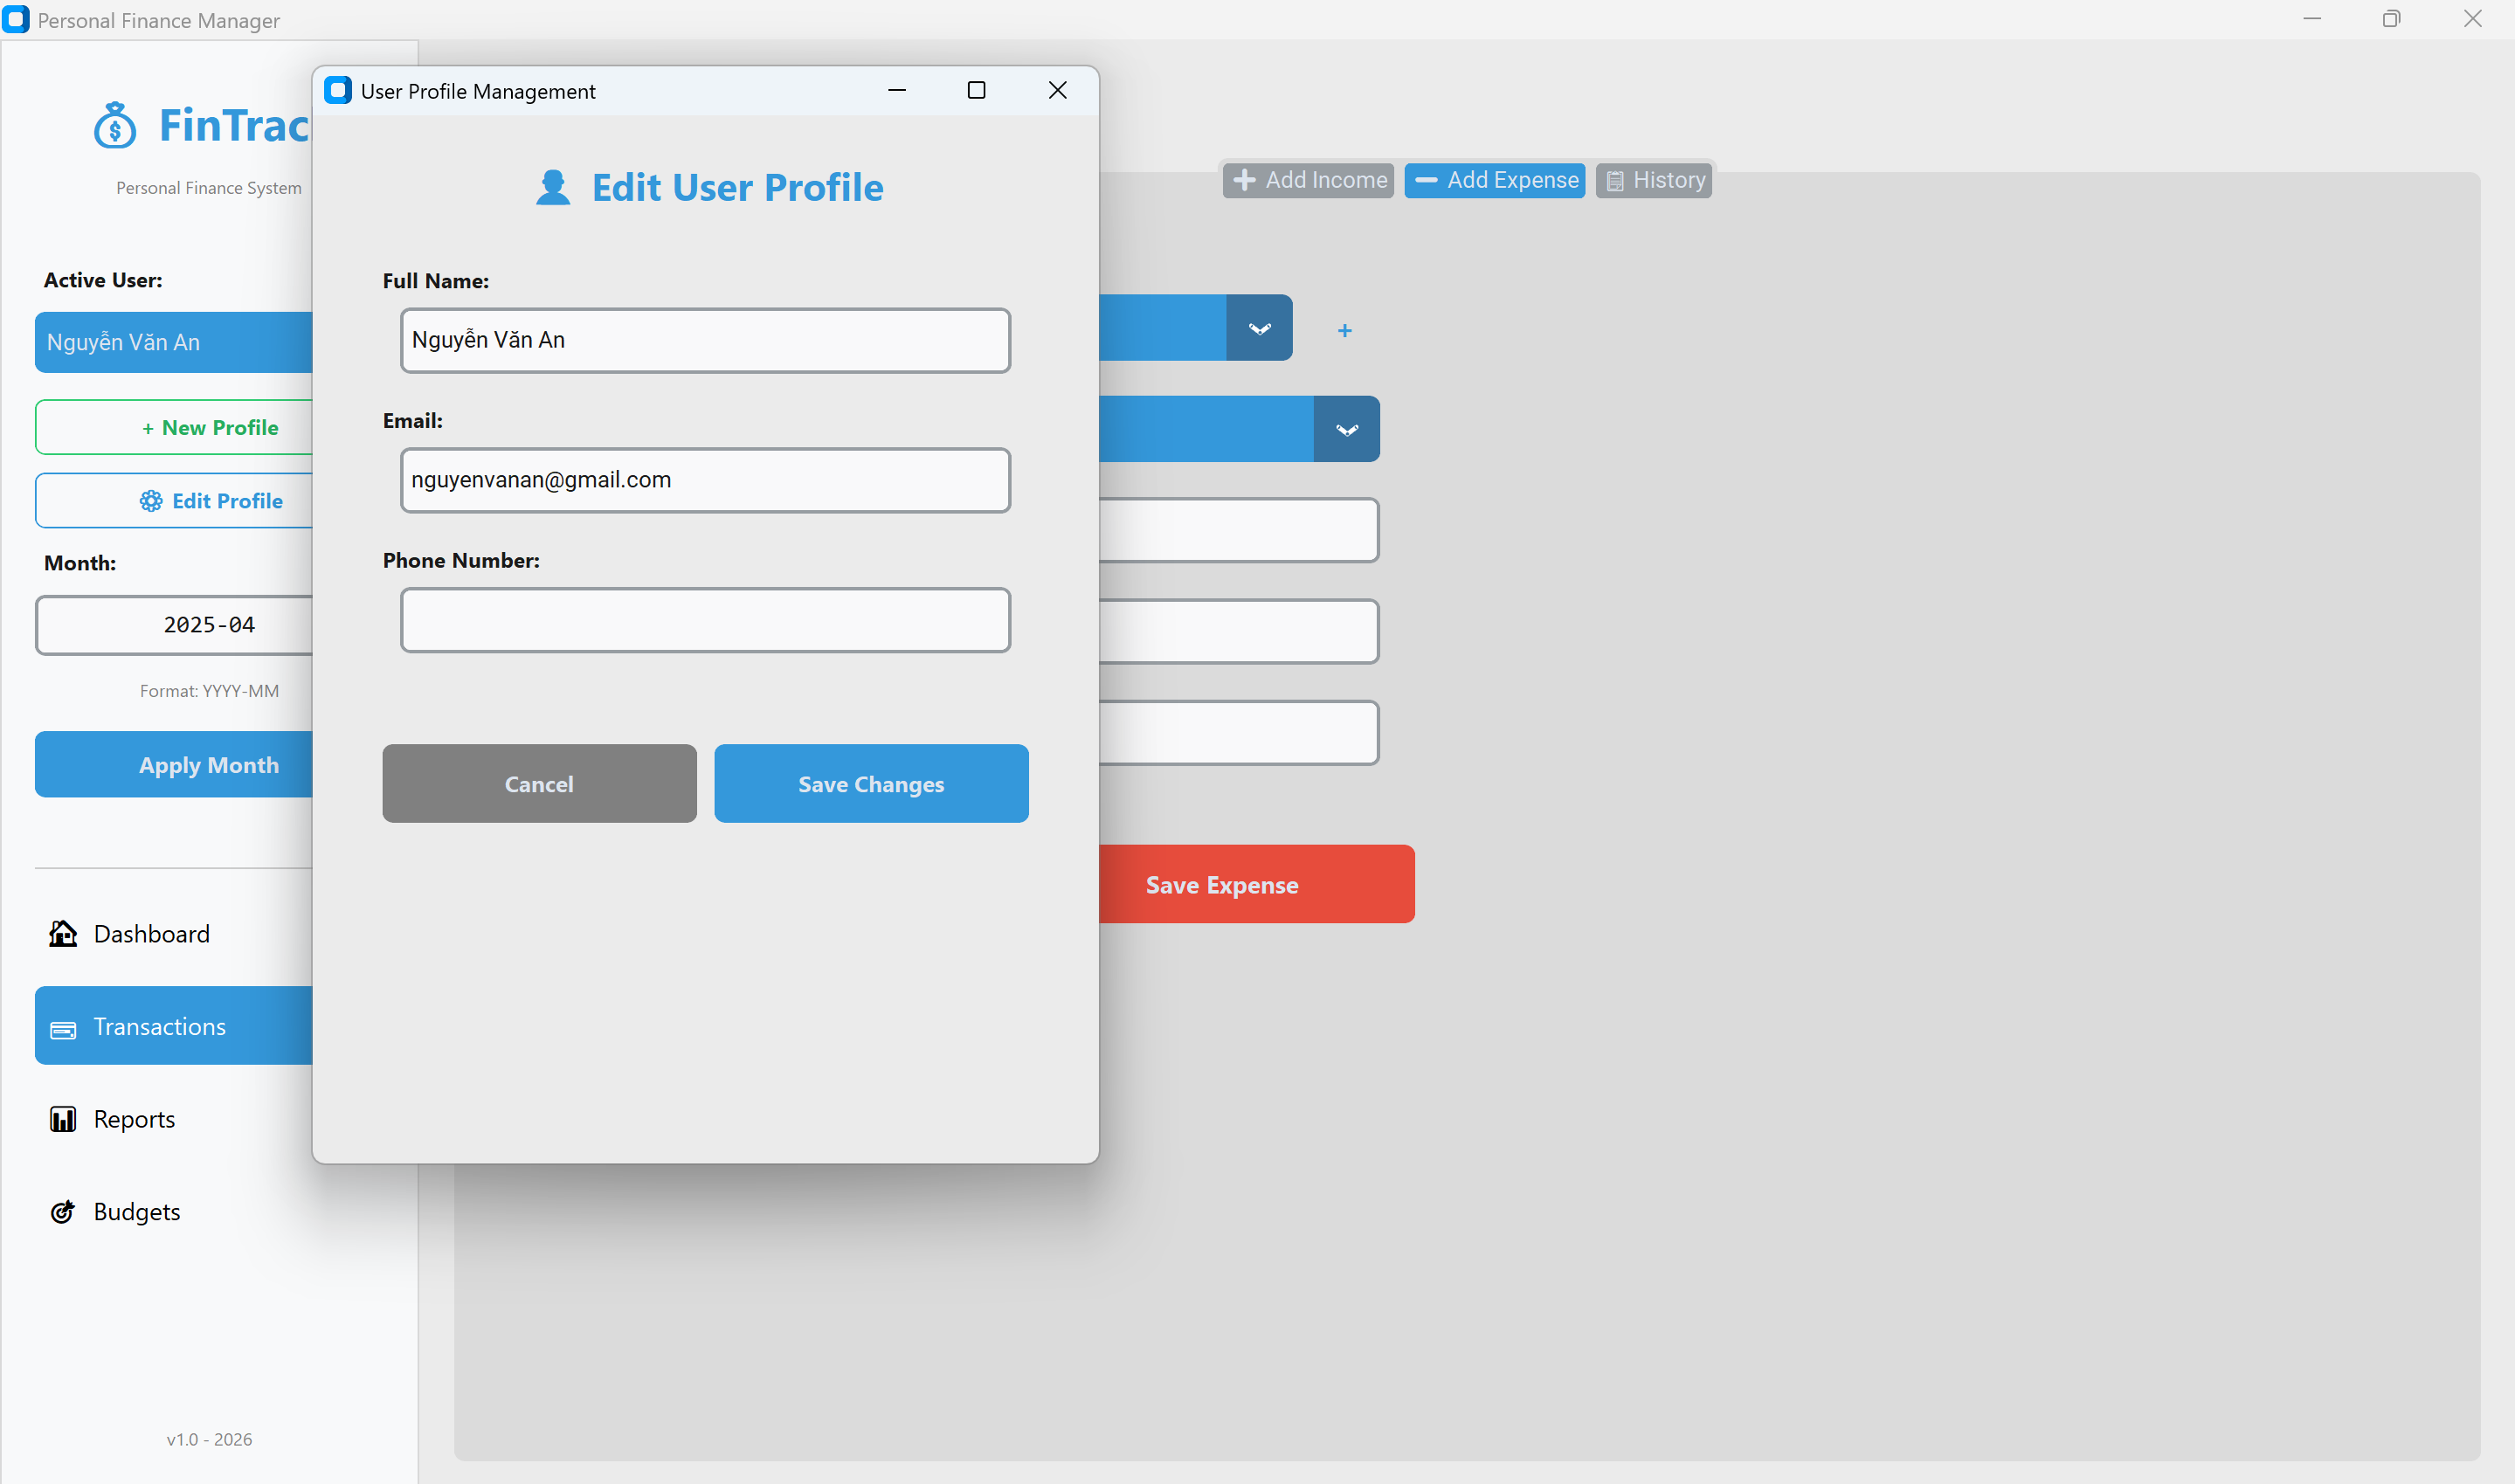
\includegraphics[width=\textwidth]{screenshot/edit_profile.png}
    \caption{Edit User Profile dialog, pre-populated with the active user's
             current data. Clicking Save Changes calls
             \texttt{update\_user\_profile()}, issuing a parameterised
             \texttt{UPDATE} on the \texttt{Users} table.}
  \end{subfigure}
  \caption{User Profile Management dialogs, accessible from the
           \textbf{+~New Profile} and \textbf{Edit Profile} buttons
           in the sidebar, available on all screens.}
\end{figure}

\subsubsection{Budget Management}

\begin{figure}[H]
  \centering
  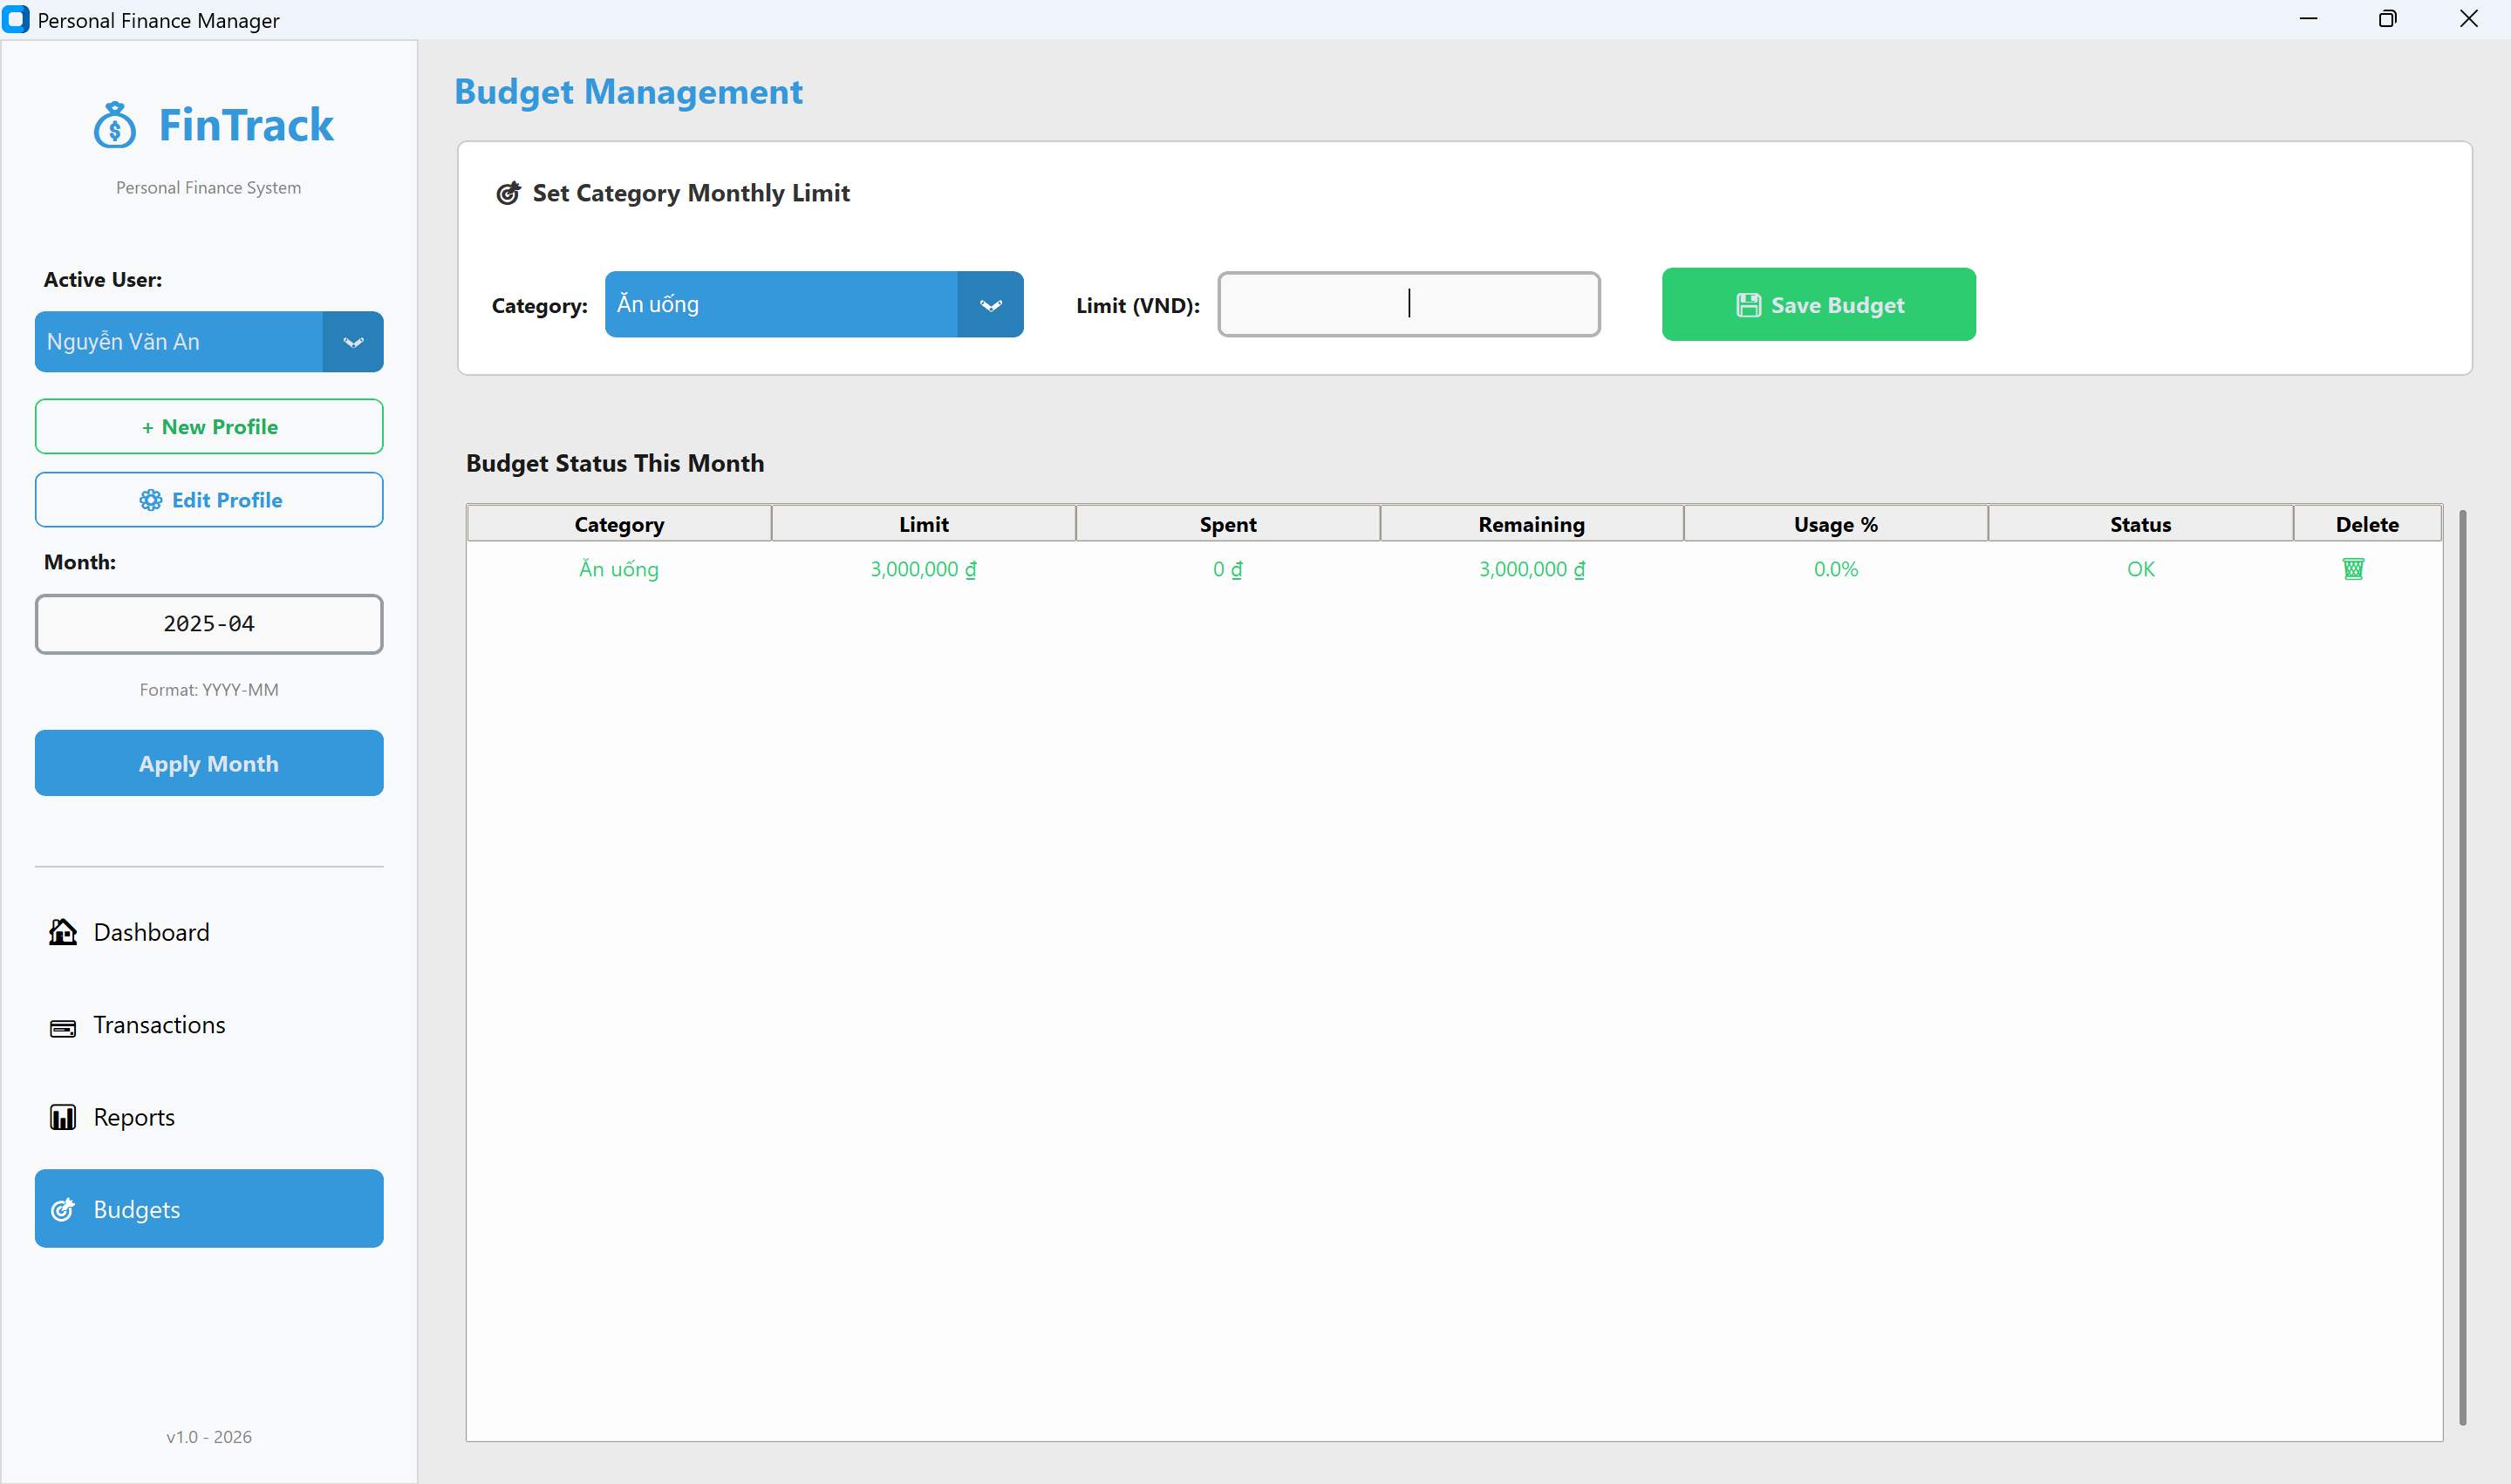
\includegraphics[width=0.92\textwidth]{screenshot/budget.png}
  \caption{Budget Management screen: a 3,000,000 VND limit is set for An uong
           (Food \& Dining) in 2025-04. The Budget Status table reads from
           \texttt{vw\_budget\_status} and displays Category, Limit, Spent,
           Remaining, Usage\%, and Status. Each row has a trash-can icon in
           the Delete column for inline budget removal.}
\end{figure}

\begin{figure}[H]
  \centering
  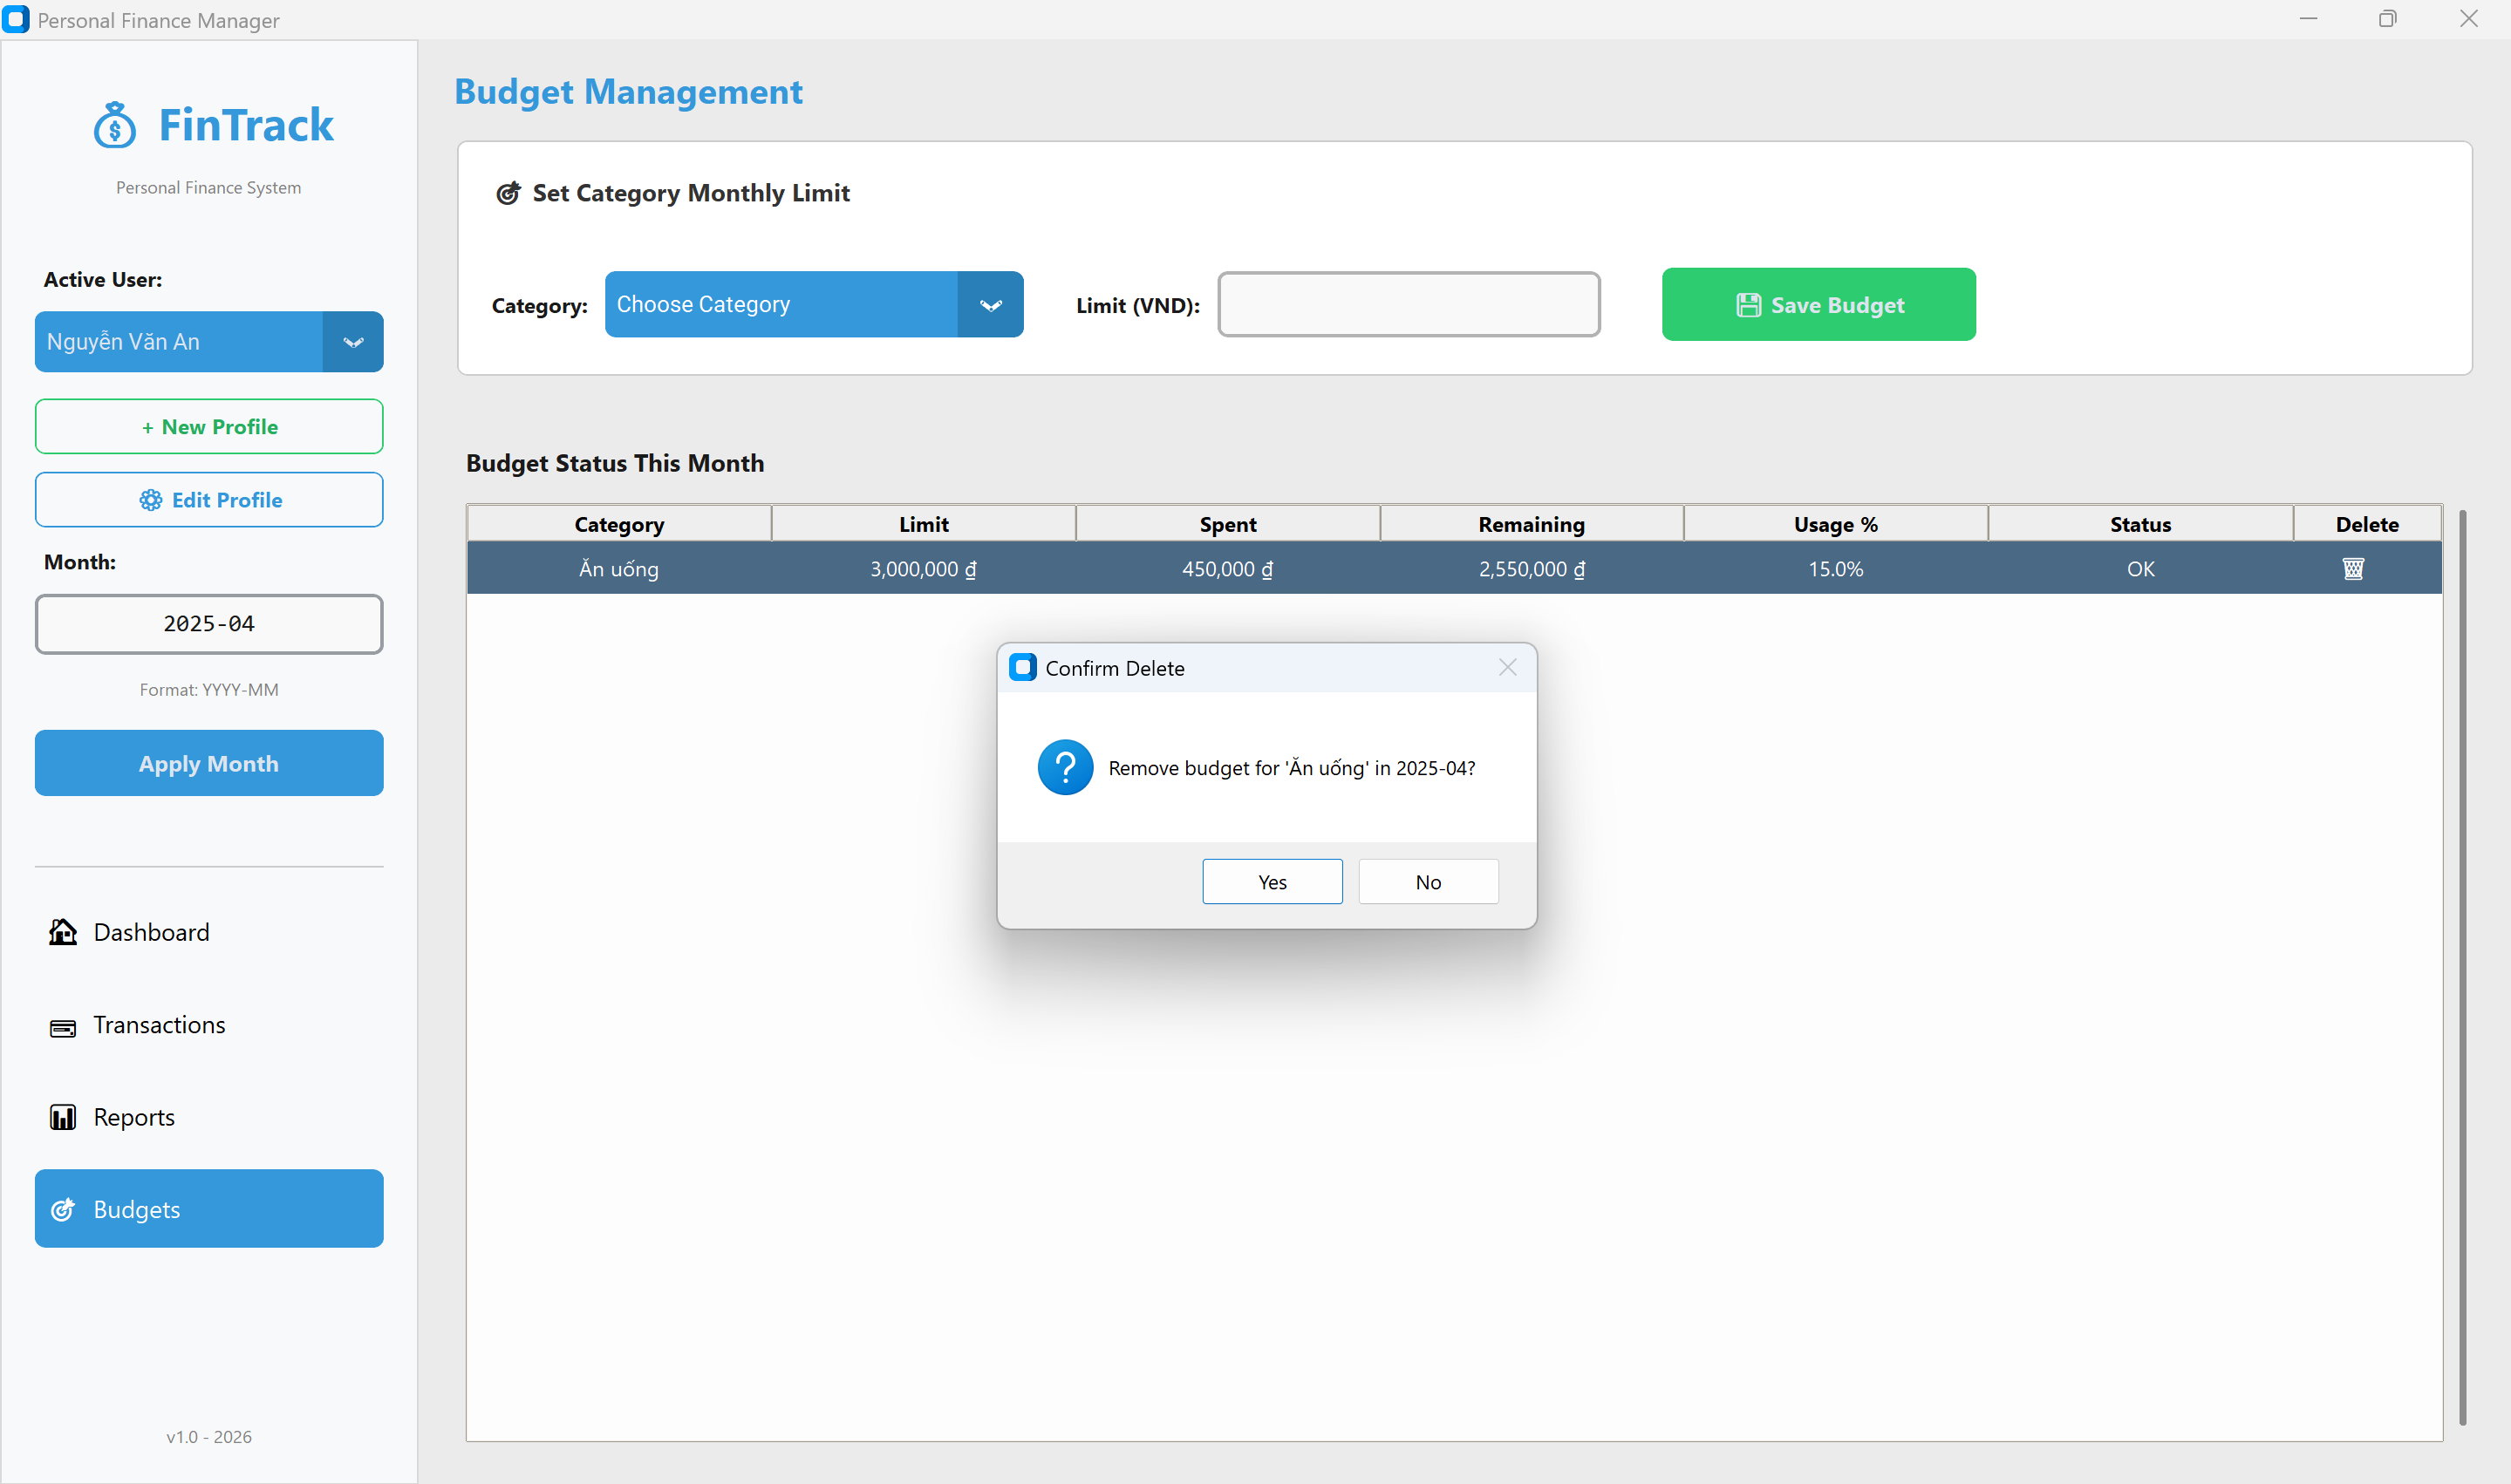
\includegraphics[width=0.85\textwidth]{screenshot/budget_delete.png}
  \caption{Budget deletion confirmation dialog. The dialog shows the category
           name and month to prevent accidental deletion. Confirming calls
           \texttt{delete\_budget(user\_id, category\_id, month\_year)}, which
           issues a \texttt{DELETE} against the \texttt{Budgets} table.
           The Budget Status table and Dashboard alerts panel both refresh
           automatically on the next screen activation.}
\end{figure}

\subsection{Reports and Analytics}

The Reports screen is divided into two tabs: \textbf{Performance Snapshots} for
numerical summaries and \textbf{Visual Analytics} for interactive charts.

\subsubsection{Performance Snapshots}

\begin{figure}[H]
  \centering
  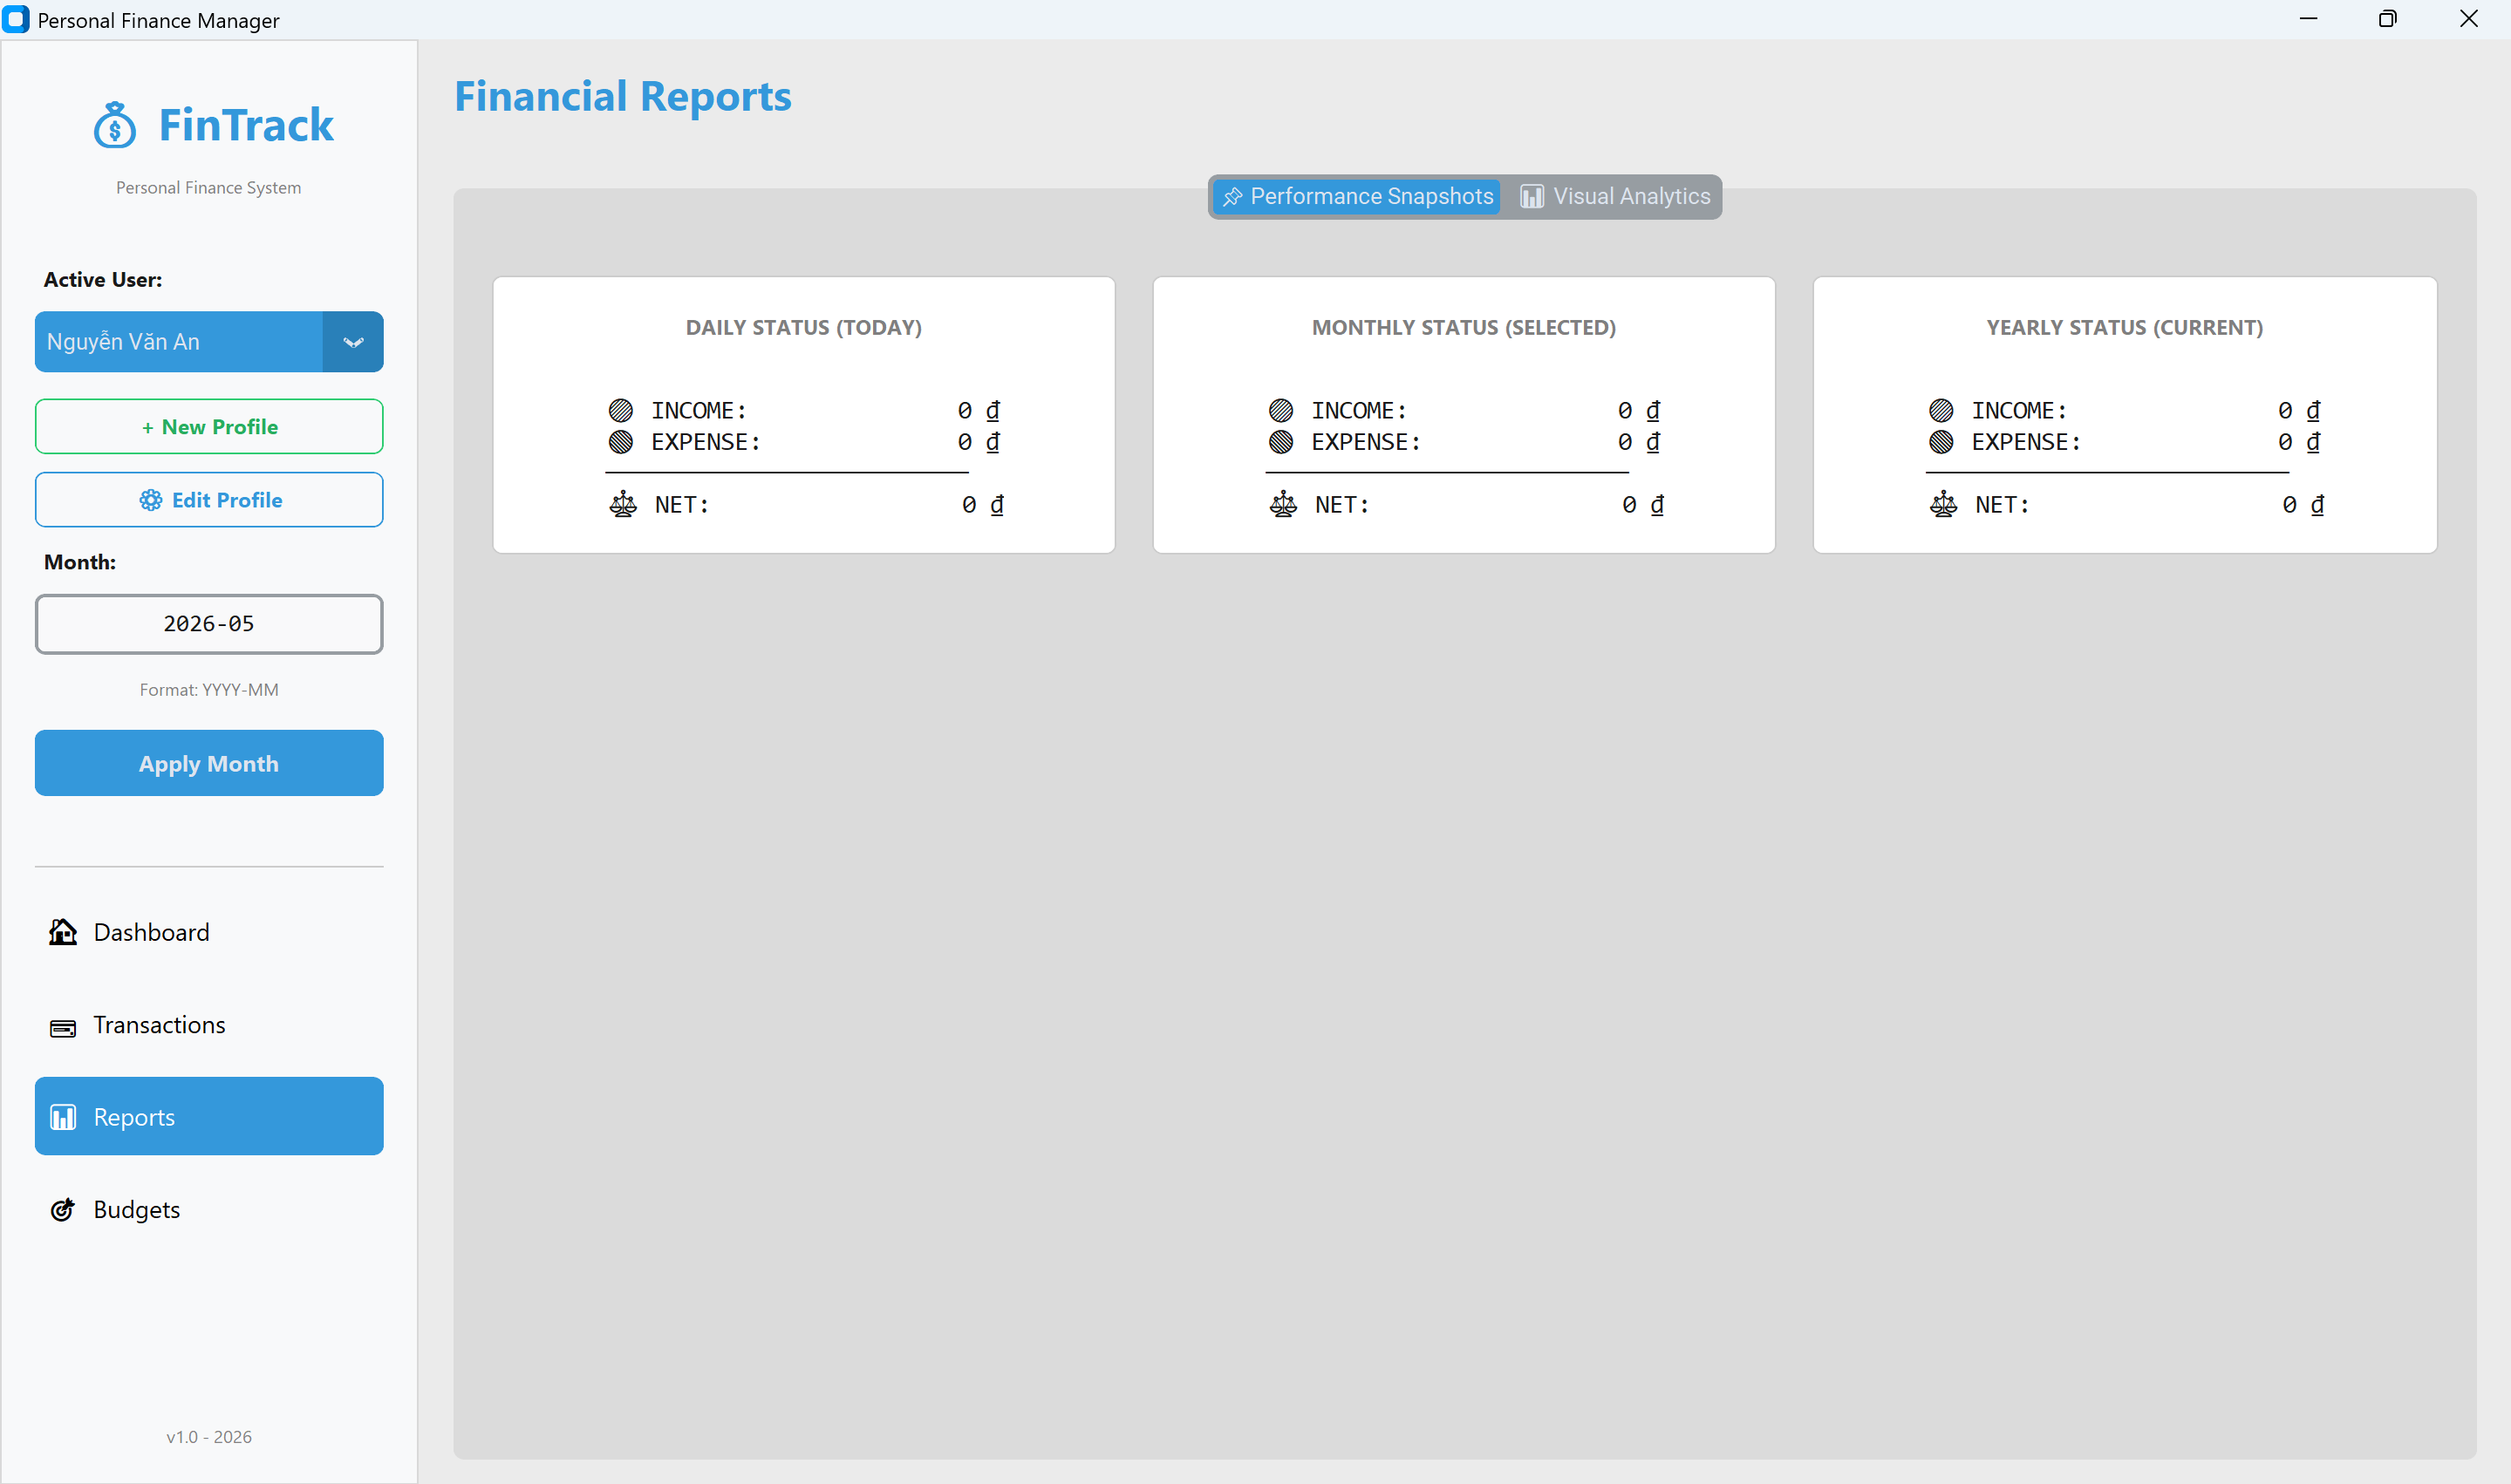
\includegraphics[width=0.92\textwidth]{screenshot/report_snapshot.png}
  \caption{Performance Snapshots tab showing three summary cards side-by-side:
           Daily Status (today via \texttt{CURDATE()}), Monthly Status (selected
           month from \texttt{vw\_monthly\_summary}), and Yearly Status (current
           year aggregated from \texttt{vw\_monthly\_summary} using a
           \texttt{LIKE} pattern). Each card shows Income, Expense, and Net figures.}
\end{figure}

\begin{table}[H]
\centering
\caption{Performance Snapshot Cards and their Data Sources}
\begin{tabularx}{\textwidth}{llX}
\toprule
\textbf{Card} & \textbf{Python Function} & \textbf{SQL Mechanism} \\
\midrule
Daily Status (Today)
  & \texttt{get\_daily\_summary()}
  & Correlated subqueries with \texttt{CURDATE()} on \texttt{Income}
    and \texttt{Expenses} tables. \\
Monthly Status (Selected)
  & \texttt{get\_monthly\_summary()}
  & Query on \texttt{vw\_monthly\_summary} filtered by selected month. \\
Yearly Status (Current)
  & \texttt{get\_yearly\_summary()}
  & Aggregation on \texttt{vw\_monthly\_summary} with
    \texttt{LIKE 'YYYY-\%'} pattern. \\
\bottomrule
\end{tabularx}
\end{table}

\subsubsection{Visual Analytics -- Monthly Income vs Expenses Bar Chart}

\begin{figure}[H]
  \centering
  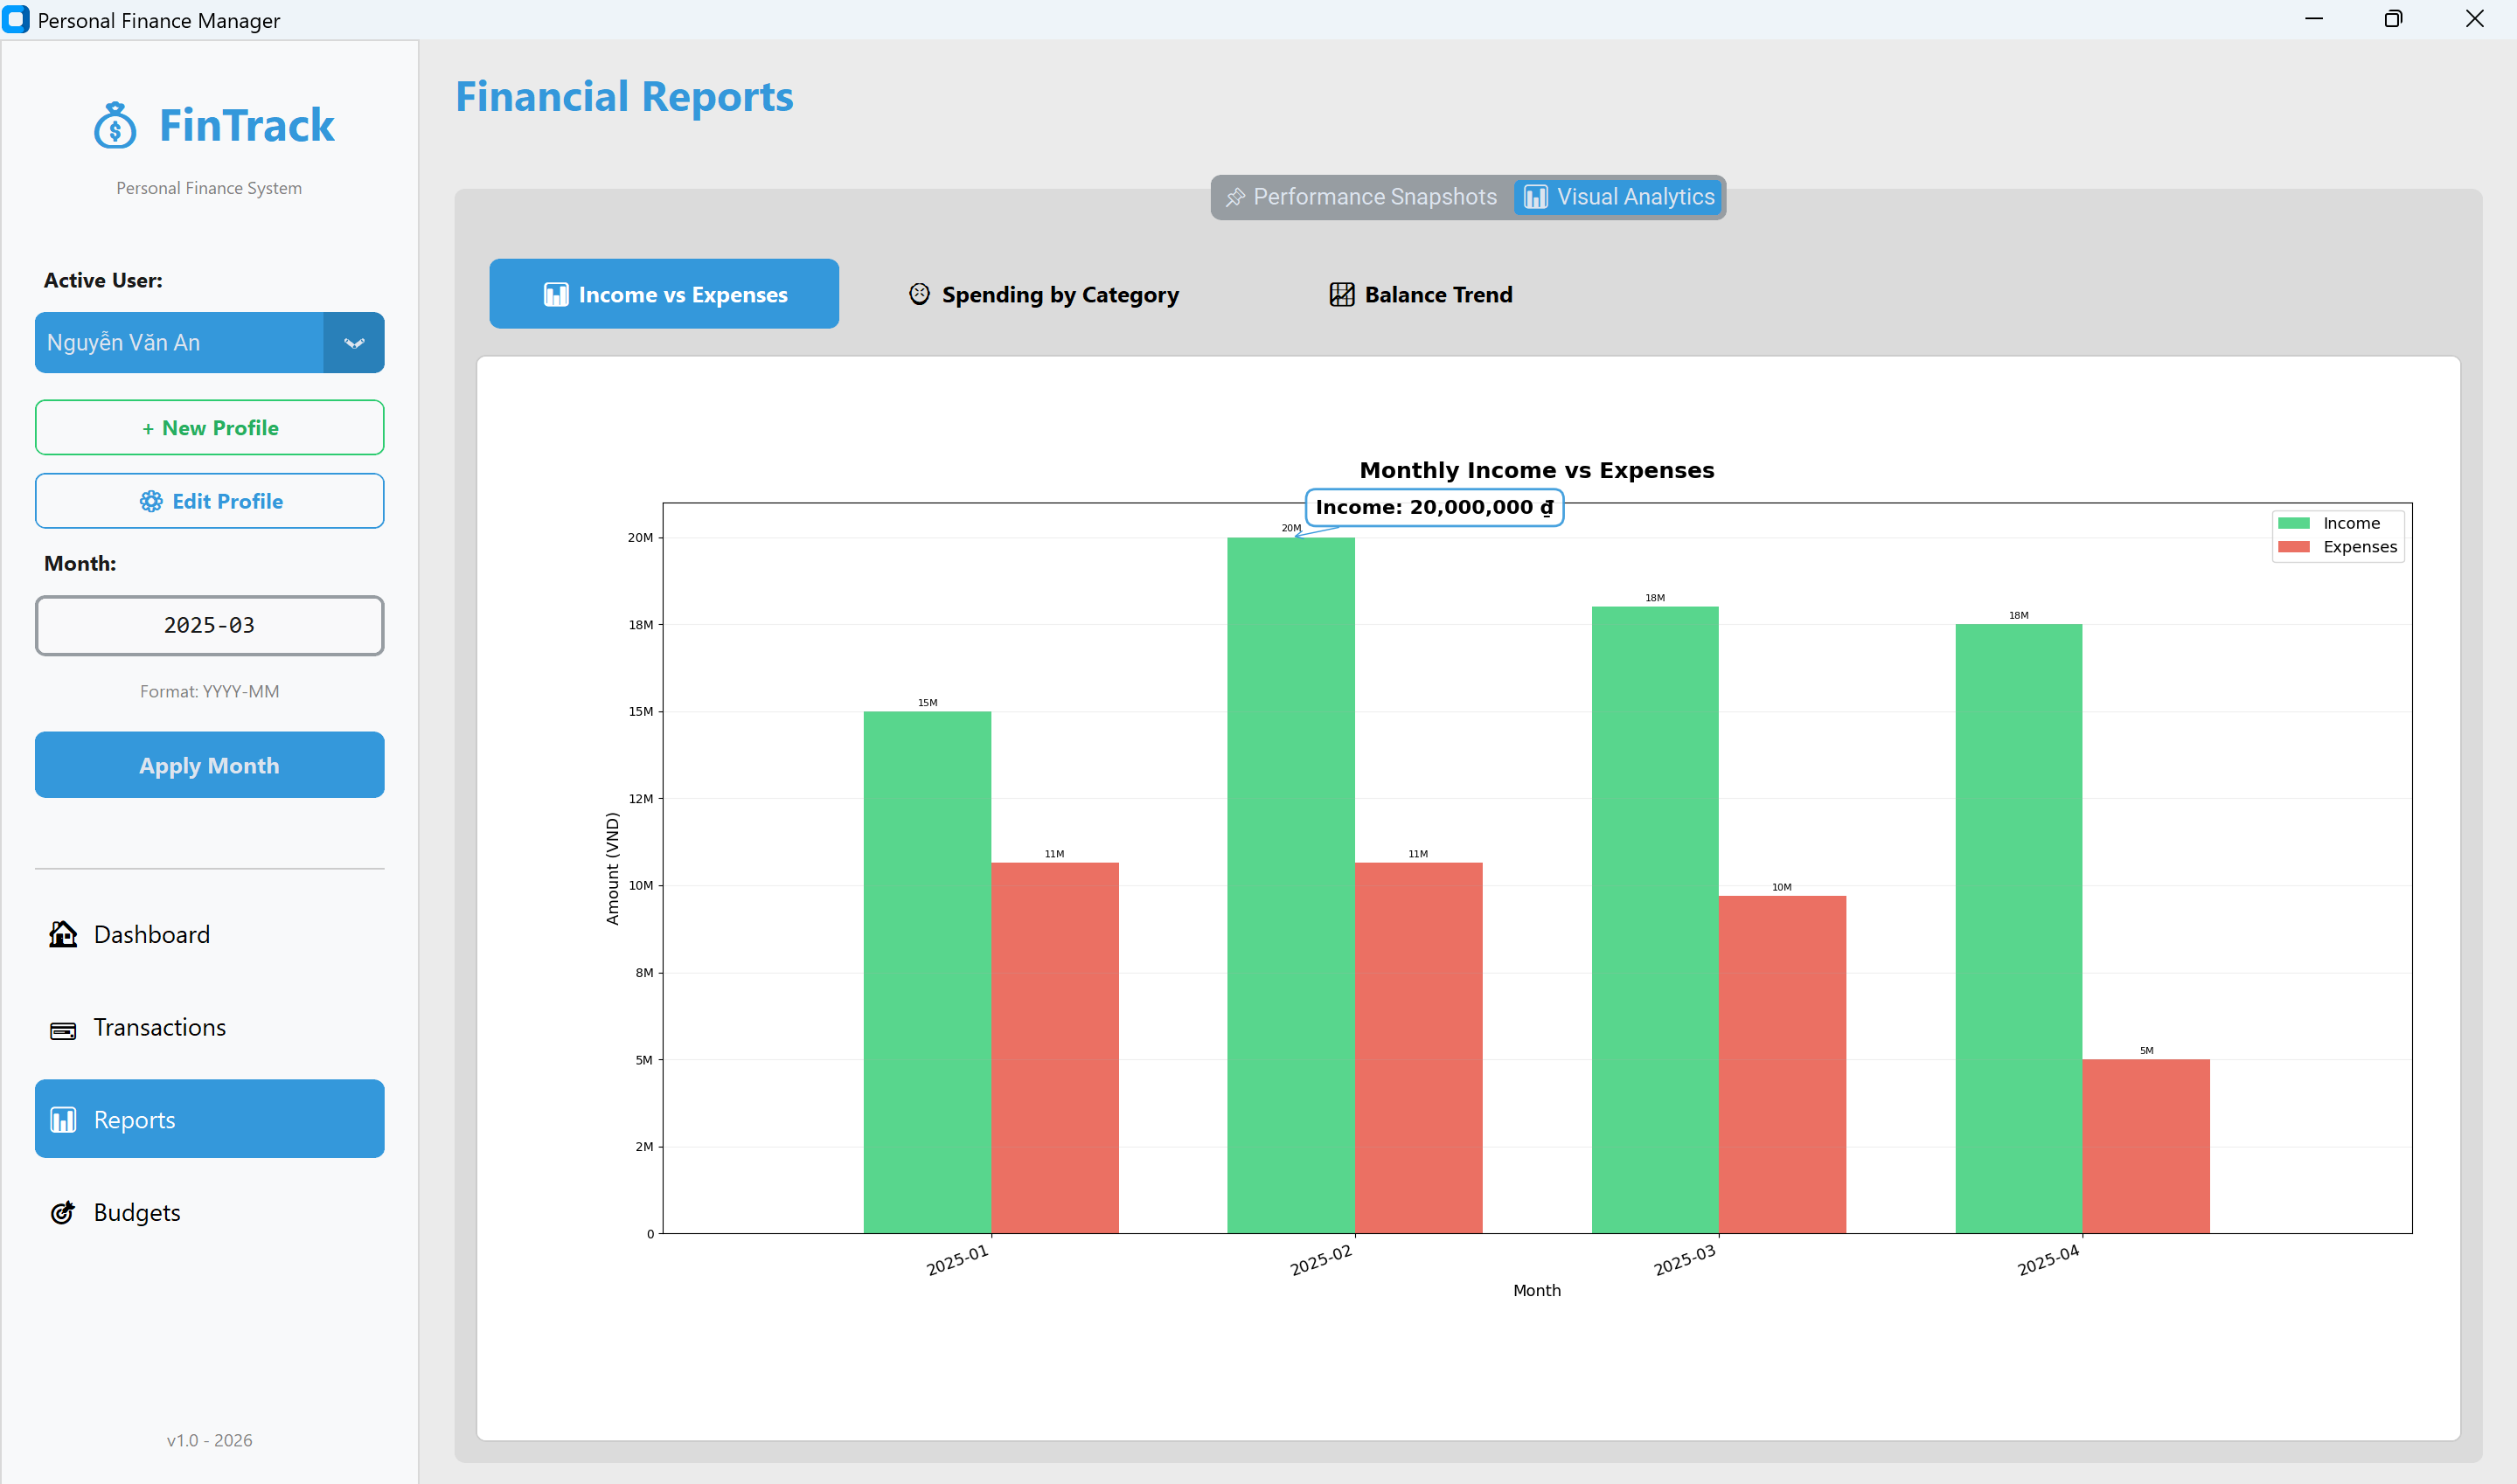
\includegraphics[width=0.95\textwidth]{screenshot/chart_bar.png}
  \caption{Income vs Expenses bar chart for months 2025-01 through 2025-04.
           Income (green) consistently exceeds expenses (red) across all months,
           indicating positive net savings. An interactive tooltip (visible above
           the 2025-02 income bar: \emph{Income: 20,000,000 d}) appears on mouse
           hover, implemented via a \texttt{motion\_notify\_event} callback in
           \texttt{main.py} that makes a hidden \texttt{matplotlib} annotation
           object visible when the cursor enters a bar region.}
\end{figure}

\subsubsection{Visual Analytics -- Spending by Category Pie Chart}

\begin{figure}[H]
  \centering
  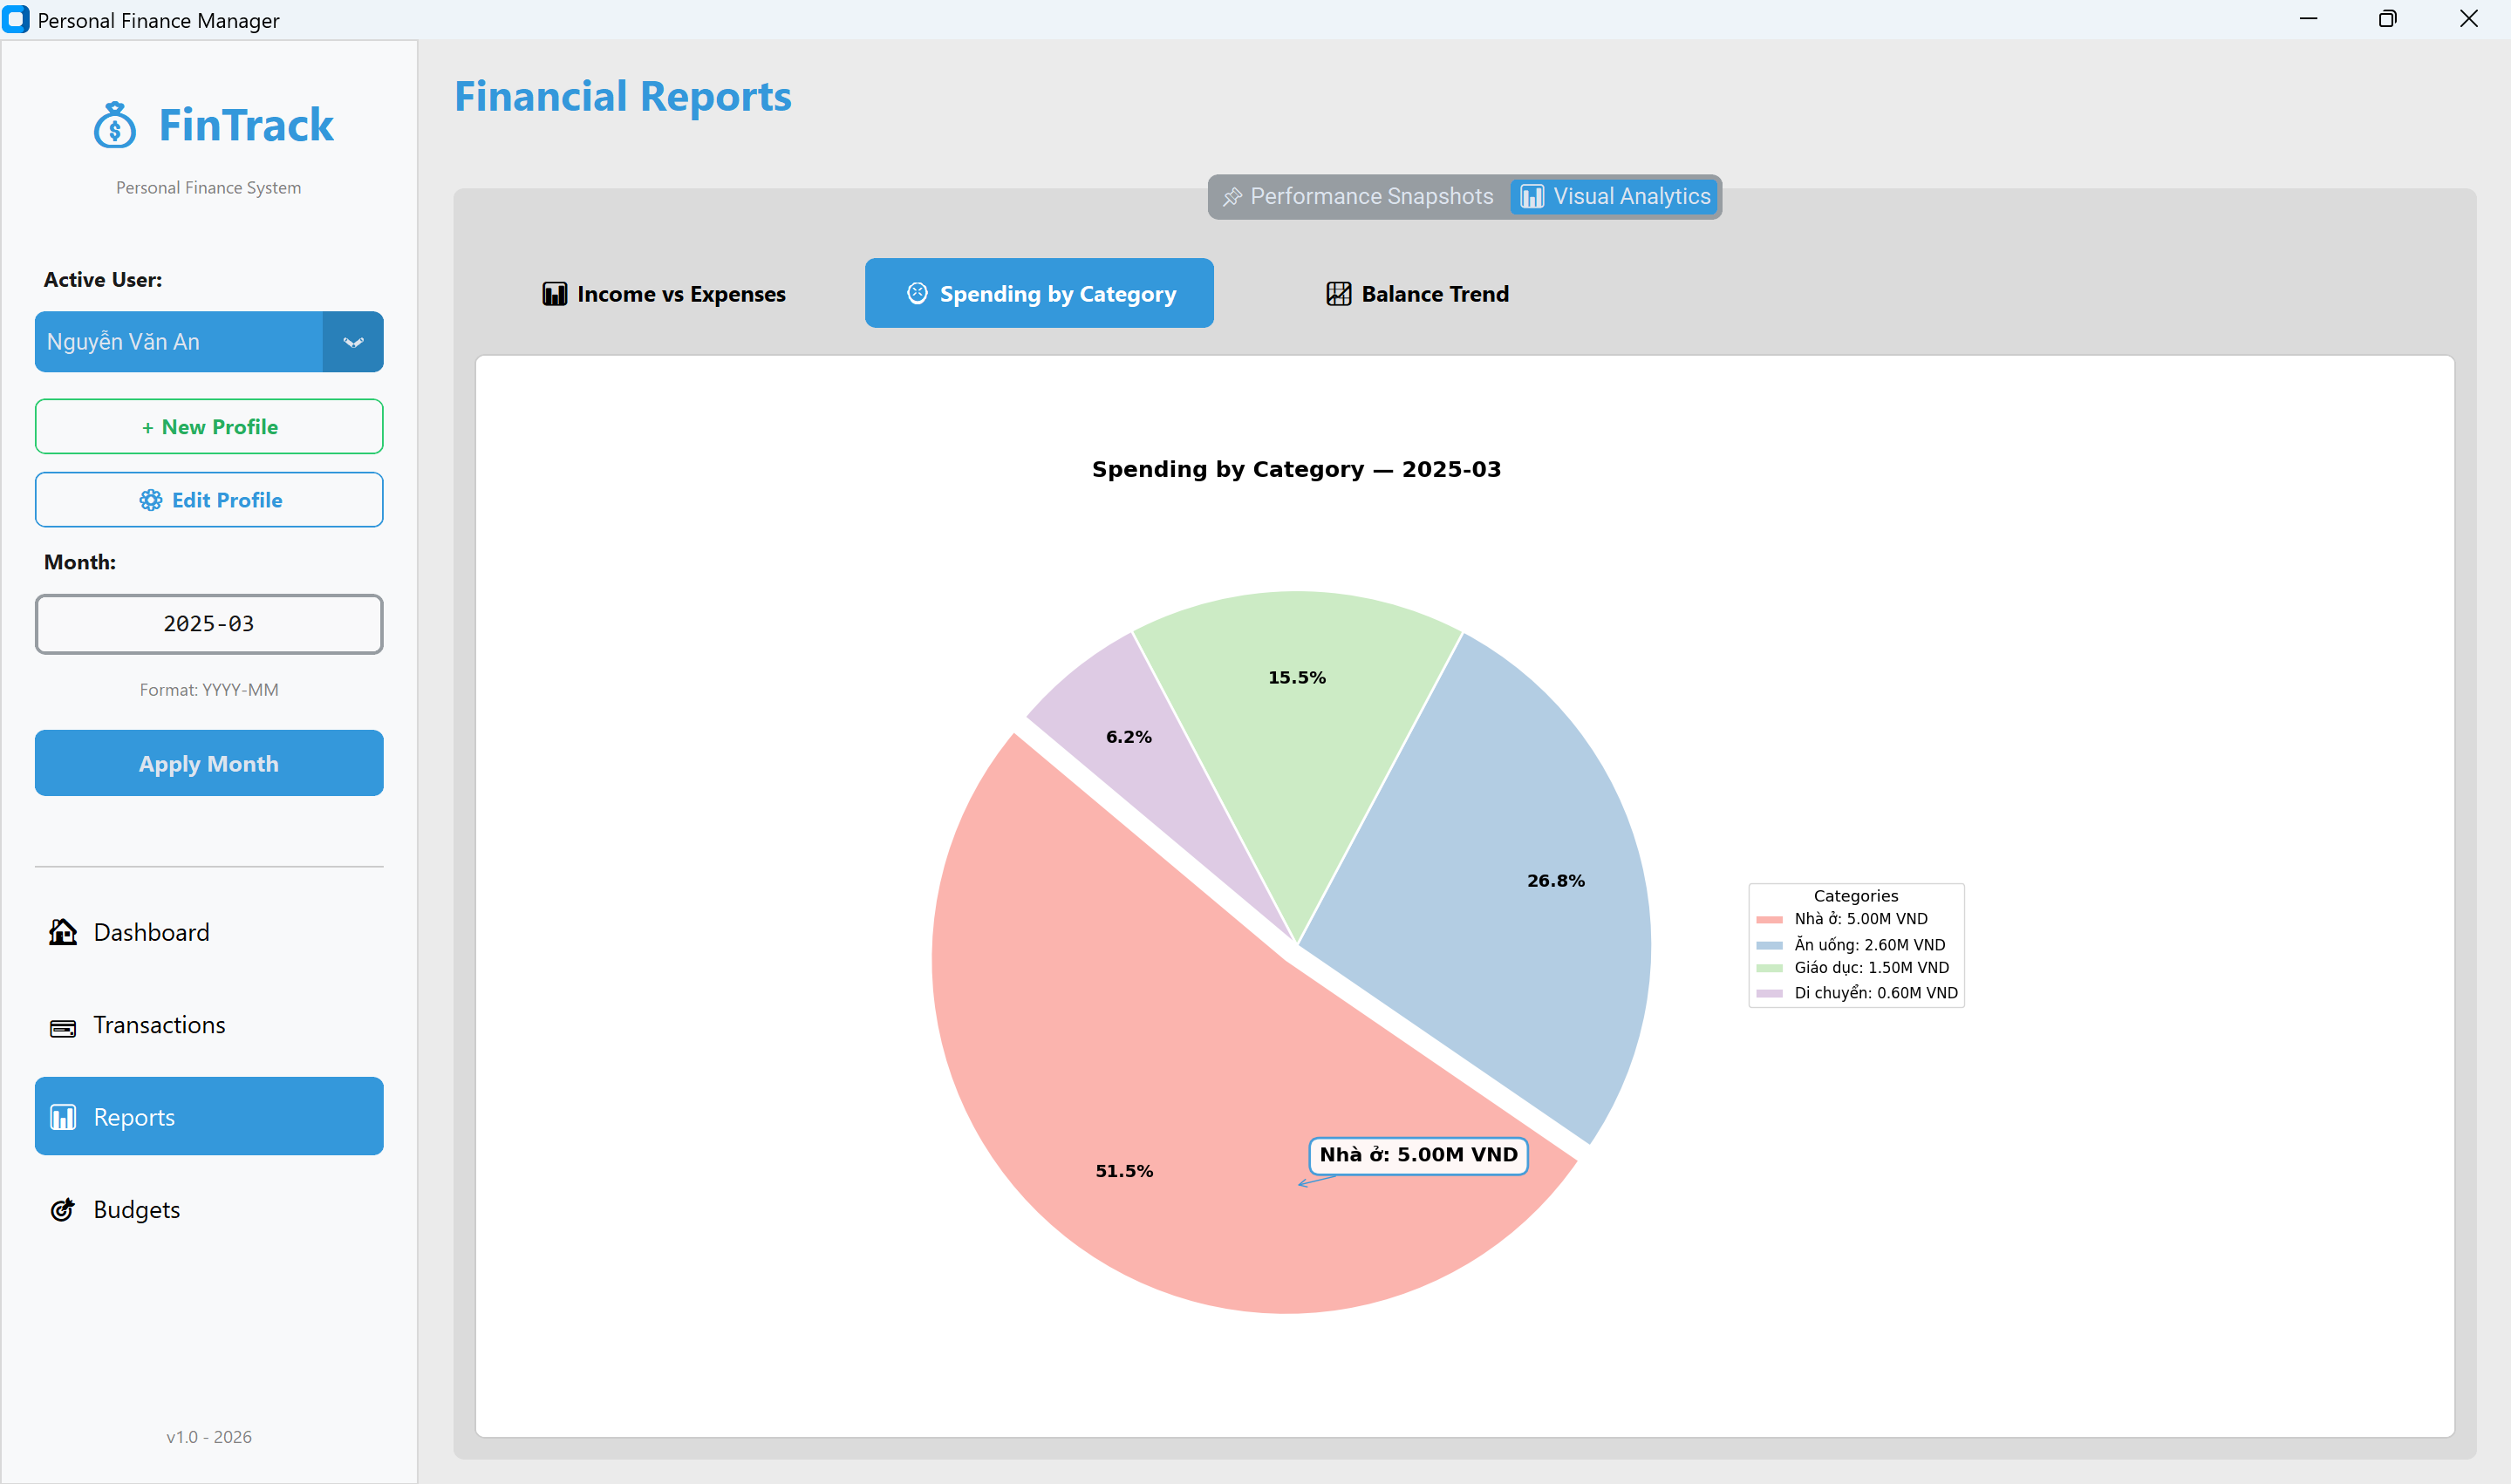
\includegraphics[width=0.85\textwidth]{screenshot/chart_pie.png}
  \caption{Category spending distribution for 2025-03. Nha o (Housing) dominates
           at 51.5\% and is slightly exploded for visual emphasis. The interactive
           tooltip shows the exact VND amount on hover (\emph{Nha o: 5.00M VND}).
           The legend lists all categories with their absolute amounts in VND.}
\end{figure}

\subsubsection{Visual Analytics -- Net Balance Trend Line Chart}

\begin{figure}[H]
  \centering
  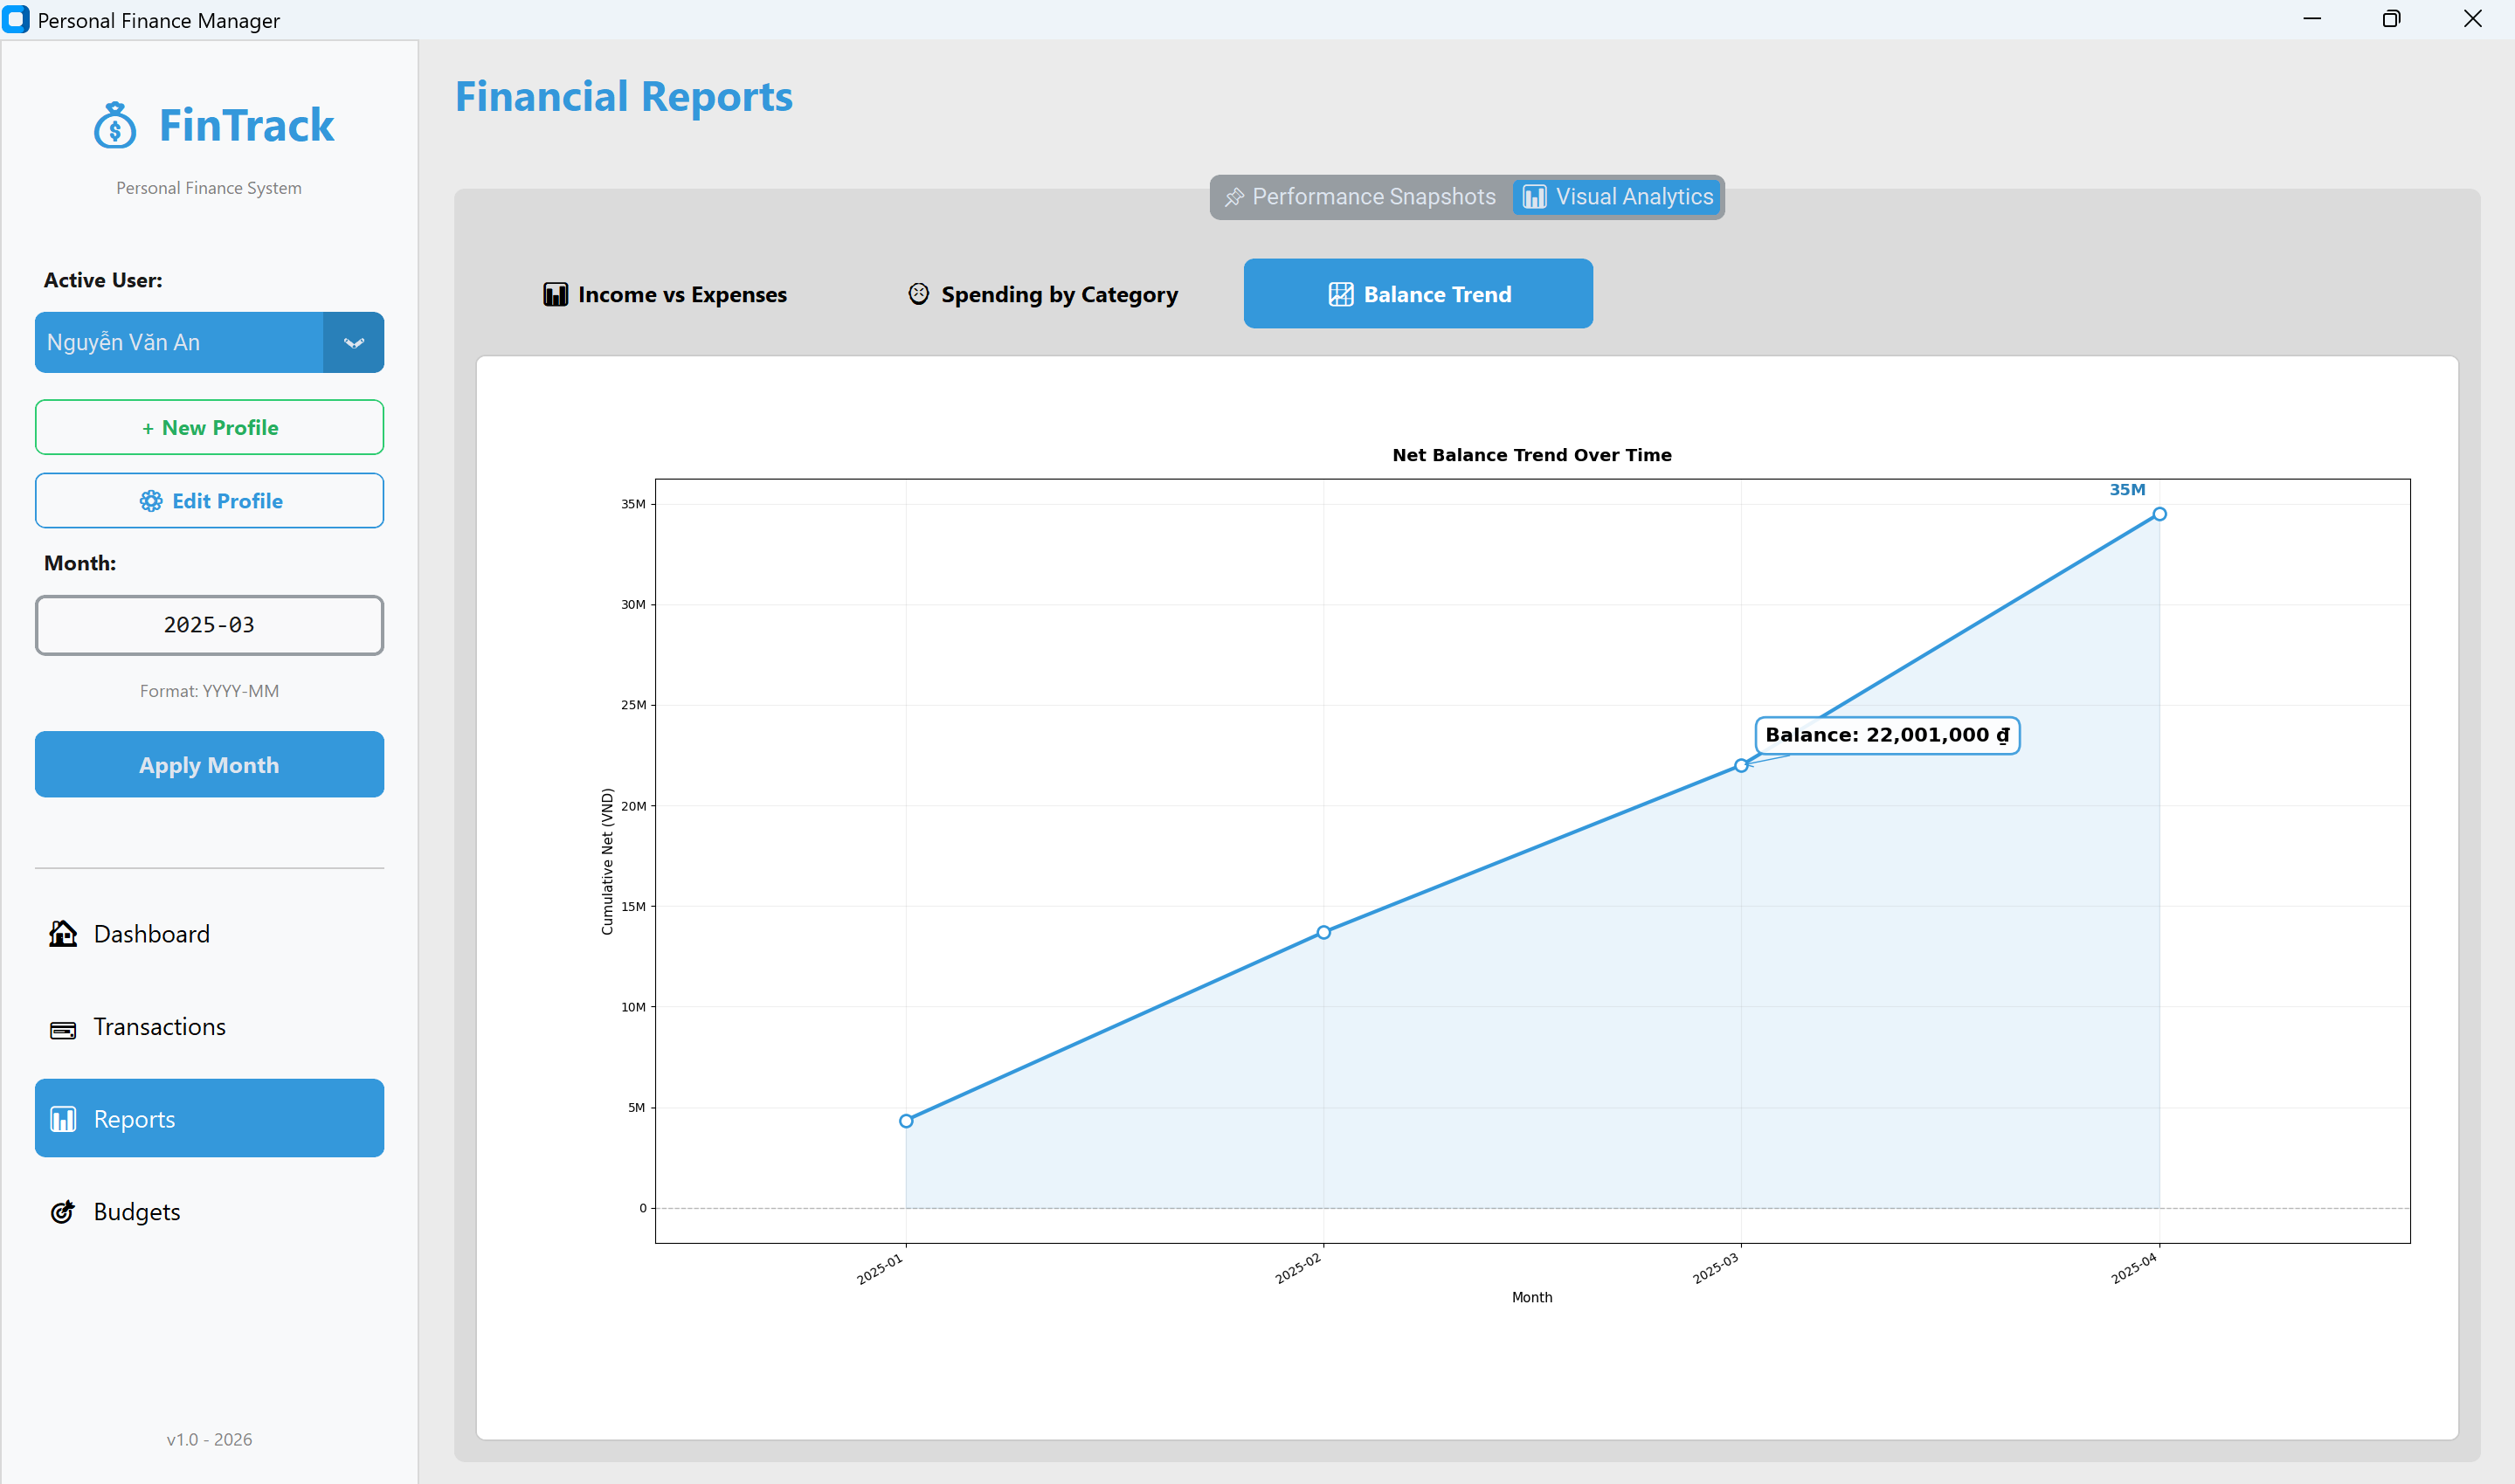
\includegraphics[width=0.95\textwidth]{screenshot/chart_line.png}
  \caption{Cumulative net balance trend from 2025-01 to 2025-04, reaching 35M VND.
           An interactive tooltip shows the exact balance at each data point on hover
           (\emph{Balance: 22,001,000 d}). The chart is built using a \texttt{UNION ALL}
           subquery that merges all income and expense events into a single timeline,
           then applies \texttt{numpy.cumsum()} to produce the running balance.
           The shaded area under the line and the zero-reference dashed line provide
           immediate visual context for whether cumulative savings are positive.}
\end{figure}

\subsection{Sample Data}

The database was populated with a large-scale, realistic Vietnamese financial dataset to ensure system performance and verify the robustness of triggers and reporting logic:

\begin{table}[H]
\centering
\caption{Sample Data Summary}
\begin{tabular}{lrl}
\toprule
\textbf{Table} & \textbf{Records} & \textbf{Notes} \\
\midrule
Users              & 50  & Diverse user base with varied professions \\
BankAccounts       & 100 & Average of 2 accounts per user (Cash and Banking) \\
ExpenseCategories  & 15  & Comprehensive categories (Food, Transport, etc.) \\
Income             & 194 & Multi-year monthly salaries and freelance records \\
Expenses           & 444 & Detailed daily transaction history (2025) \\
Budgets            & 323 & Monthly category-wise spending limits across users \\
\bottomrule
\end{tabular}
\end{table}

\newpage

% ============================================================
\section{Analysis, Evaluation and Discussion}
% ============================================================

\subsection{Functional Verification}

Each requirement was verified through manual testing:

\begin{table}[H]
\centering
\caption{Functional Requirement Test Results}
\begin{tabular}{llp{7.5cm}l}
\toprule
\textbf{ID} & \textbf{Feature} & \textbf{Test Action} & \textbf{Result} \\
\midrule
FR-03 & Income trigger    & Inserted 17,500,000 VND; balance incremented correctly
  & \textcolor{codegreen}{\textbf{PASS}} \\
FR-04 & Expense trigger   & Inserted 5,000,000 VND; balance decremented correctly
  & \textcolor{codegreen}{\textbf{PASS}} \\
FR-05 & Budget CRUD       & Set, updated, and deleted a 2,000,000 VND Food budget
  & \textcolor{codegreen}{\textbf{PASS}} \\
FR-06 & Budget alert      & 95\% Food usage $\to$ WARNING displayed on Dashboard
  & \textcolor{codegreen}{\textbf{PASS}} \\
FR-07 & Monthly report    & \texttt{vw\_monthly\_summary} returns correct aggregates
  & \textcolor{codegreen}{\textbf{PASS}} \\
FR-08 & Stored proc.      & \texttt{CALL sp\_monthly\_report(1,'2025-01')} returns 2 result sets
  & \textcolor{codegreen}{\textbf{PASS}} \\
FR-09 & UDF               & \texttt{SELECT fn\_get\_total\_expenses (1,'2025-01')} = 10,970,000
  & \textcolor{codegreen}{\textbf{PASS}} \\
FR-10 & GUI navigation    & All 4 screens load without errors; data refreshes on activation
  & \textcolor{codegreen}{\textbf{PASS}} \\
FR-11 & Daily/yearly      & Dashboard shows today's figures; yearly aggregation correct
  & \textcolor{codegreen}{\textbf{PASS}} \\
FR-12 & Income/Expense CRUD & Edit and delete income/expense; balance updated by trigger
  & \textcolor{codegreen}{\textbf{PASS}} \\
FR-13 & Category \& profile & New category added inline; user profile updated without error
  & \textcolor{codegreen}{\textbf{PASS}} \\
\bottomrule
\end{tabular}
\end{table}

\subsection{Trigger Correctness Verification}

The trigger mechanism was verified directly in MySQL Workbench:

\begin{lstlisting}[style=sqlstyle, caption={Trigger Verification Queries}]
-- Step 1: Record initial balance
SELECT AccountID, BankName, Balance
FROM BankAccounts WHERE AccountID = 1;
-- Result: Vietcombank | 45,000,000.00

-- Step 2: Insert income
INSERT INTO Income 
(UserID, AccountID, Amount, IncomeDate, Description)
VALUES (1, 1, 1000000, '2025-04-01', 'Trigger test');

-- Step 3: Verify balance incremented
SELECT Balance FROM BankAccounts WHERE AccountID = 1;
-- Result: 46,000,000.00  (+1,000,000 -- trigger fired correctly)

-- Step 4: Insert expense
INSERT INTO Expenses
(UserID, CategoryID, AccountID, Amount, ExpenseDate, Description)
VALUES (1, 1, 1, 500000, '2025-04-01', 'Trigger test');

-- Step 5: Verify balance decremented
SELECT Balance FROM BankAccounts WHERE AccountID = 1;
-- Result: 45,500,000.00  (-500,000 -- trigger fired correctly)
\end{lstlisting}

\subsection{Evaluation Against Requirements}

\subsubsection{What Worked Well}

\begin{enumerate}[leftmargin=2em]
  \item \textbf{Full lifecycle trigger integrity:} All six triggers correctly maintained
        balance consistency across INSERT, UPDATE, and DELETE scenarios. The UPDATE
        triggers handle both same-account amount changes and cross-account transfers
        using a dual-case \texttt{IF/ELSEIF} structure. Because the logic lives in
        MySQL, the invariant holds even if the database is accessed directly through
        MySQL Workbench or the CLI.

  \item \textbf{Budget alert system:} The \texttt{vw\_budget\_status} view encapsulates
        a non-trivial multi-table aggregation with conditional logic (\texttt{CASE}
        expression). The Python layer simply queries the view; adding a new status tier
        (e.g.\ 90\% ``CRITICAL'') would require only a change to the view definition.

  \item \textbf{Separation of concerns:} No SQL string exists in \texttt{main.py}.
        The four-file architecture cleanly separates presentation, business logic,
        reporting, and data access. This made debugging significantly easier -- a chart
        rendering bug and a balance display bug were both isolated and fixed without
        touching the database layer.

  \item \textbf{Realistic sample data:} Salaries, rent, grocery, and transport amounts
        were calibrated against Vietnamese living-cost statistics, making the system
        credible for demonstration purposes.

  \item \textbf{Interactive tooltips on all charts:} All three matplotlib charts
        implement hover tooltips via a hidden \texttt{annotate} object that becomes
        visible when the mouse enters a bar, wedge, or data point. This was implemented
        entirely in \texttt{main.py} using \texttt{mpl\_connect('motion\_notify\_event')}
        without modifying \texttt{reports.py}, demonstrating clean separation between
        chart generation and UI interaction logic.

  \item \textbf{Dual-granularity reporting:} The Performance Snapshots tab provides
        daily, monthly, and yearly figures simultaneously, satisfying the requirement
        for multiple financial summary granularities without requiring additional
        database objects beyond the existing \texttt{vw\_monthly\_summary} view and
        a \texttt{CURDATE()} subquery.
\end{enumerate}

\subsubsection{Limitations and Known Issues}

\begin{enumerate}[leftmargin=2em]
  \item \textbf{MySQL \texttt{\%} escaping:} \texttt{mysql-connector-python} escapes
        all \texttt{\%} characters in the parameterised \texttt{cursor.execute()} path.
        Queries using \texttt{DATE\_FORMAT(col, '\%Y-\%m')} inside the generic
        \texttt{execute\_query} helper produced \texttt{'\%\%Y-\%\%m'} at runtime.
        The fix was to bypass the helper for affected queries and use direct connection
        objects. A cleaner long-term solution would be to replace
        \texttt{DATE\_FORMAT} with \texttt{YEAR(col)} and \texttt{MONTH(col)}.

  \item \textbf{No authentication layer:} User selection is handled via a dropdown.
        A production system would require bcrypt-hashed passwords and a login screen.

  \item \textbf{Single-machine deployment:} The application connects to
        \texttt{localhost} only. A shared deployment would require a networked MySQL
        instance with TLS encryption.

  \item \textbf{Generic error messages on constraint violation:} If the
        \texttt{BankAccounts} \texttt{CHECK} constraint rejects an expense, the
        application displays a generic error. A more robust implementation would
        catch MySQL error code 3819 and display a user-friendly
        ``Insufficient balance'' message.

  \item \textbf{No concurrency control:} The helper opens a new connection per call,
        which is safe for single-user desktop use. A multi-user deployment would
        require connection pooling and explicit transaction isolation levels.
\end{enumerate}

\subsection{Comparison: Database-Layer vs Application-Layer Business Logic}

\begin{table}[H]
\centering
\caption{Database Layer vs Application Layer Trade-offs}
\begin{tabularx}{\textwidth}{Xll}
\toprule
\textbf{Concern} & \textbf{Chosen Layer} & \textbf{Rationale} \\
\midrule
Balance update after transaction & MySQL Trigger      & Guaranteed regardless of access method \\
Budget usage calculation         & MySQL View + UDF   & Single source of truth; no duplication \\
Monthly report aggregation       & MySQL Stored Proc  & Complex SQL kept in one place \\
Chart rendering                  & Python (matplotlib)& Database cannot generate visual output \\
UI event handling                & Python (tkinter)   & Desktop GUI requires application code \\
Input validation (format)        & Python             & Faster feedback before DB round-trip \\
\bottomrule
\end{tabularx}
\end{table}

\subsection{Future Improvement Directions}

\begin{enumerate}[leftmargin=2em]
  \item \textbf{Savings goals module:} Add a \texttt{SavingsGoals} table
        (\texttt{GoalName}, \texttt{TargetAmount}, \texttt{Deadline}) and a trigger
        that checks remaining balance against active goals after each expense.
  \item \textbf{Exchange rate API integration:} Connect to an open exchange-rate API
        to support multi-currency income with automatic conversion to VND at the date
        of receipt.
  \item \textbf{PDF report export:} Use the \texttt{reportlab} library to export the
        monthly financial report as a professionally formatted PDF.
  \item \textbf{Email / push notifications:} Send a monthly summary email using
        Python's \texttt{smtplib} when a budget reaches 80\% or 100\%.
  \item \textbf{Predictive analytics:} Apply a simple linear regression on the
        \texttt{vw\_monthly\_summary} data to project next month's expenses by
        category, alerting users in advance if a budget overrun is likely.
\end{enumerate}

\newpage

% ============================================================
\section{Report Quality, Presentation and Academic Standards}
% ============================================================

\subsection{Deliverables Checklist}

\begin{table}[H]
\centering
\caption{Project Deliverables}
\begin{tabularx}{\textwidth}{llX}
\toprule
\textbf{Deliverable} & \textbf{Status} & \textbf{Location} \\
\midrule
ER Diagram
  & \textcolor{codegreen}{\checkmark\ Complete} & ERDPlus export (PNG) \\
\texttt{schema.sql}
  & \textcolor{codegreen}{\checkmark\ Complete} & \texttt{database/schema.sql} \\
\texttt{sample\_data.sql}
  & \textcolor{codegreen}{\checkmark\ Complete} & \texttt{database/sample\_data.sql} \\
\texttt{objects.sql}
  & \textcolor{codegreen}{\checkmark\ Complete} & \texttt{database/objects.sql} \\
\texttt{security.sql}
  & \textcolor{codegreen}{\checkmark\ Complete} & \texttt{database/security.sql} \\
\texttt{db\_connection.py}
  & \textcolor{codegreen}{\checkmark\ Complete} & \texttt{app/db\_connection.py} \\
\texttt{models.py}
  & \textcolor{codegreen}{\checkmark\ Complete} & \texttt{app/models.py} \\
\texttt{reports.py}
  & \textcolor{codegreen}{\checkmark\ Complete} & \texttt{app/reports.py} \\
\texttt{main.py}
  & \textcolor{codegreen}{\checkmark\ Complete} & \texttt{app/main.py} \\
GitHub repository 
  & \textcolor{codegreen}{\checkmark\ Complete} & \url{https://github.com/phngan23/Personal_Finance_Management_System} \\
YouTube demo video 
  & \textcolor{codegreen}{\checkmark\ Complete} & \url{https://youtube.com/YOUR_LINK} \\
This report (PDF)
  & \textcolor{codegreen}{\checkmark\ Complete} & Submitted via LMS \\
\bottomrule
\end{tabularx}
\end{table}

\subsection{Technology Stack Summary}

\begin{table}[H]
\centering
\caption{Technology Stack}
\begin{tabular}{ll}
\toprule
\textbf{Component} & \textbf{Technology} \\
\midrule
Database server        & MySQL 8.0 \\
Database design tool   & MySQL Workbench 8.0 \\
Programming language   & Python 3.x \\
DB connector library   & mysql-connector-python 8.x \\
GUI framework          & CustomTkinter 5.x \\
Chart library          & Matplotlib 3.x \\
Chart embedding        & FigureCanvasTkAgg (TkAgg backend) \\
Numerical library      & NumPy \\
IDE                    & Visual Studio Code \\
Version control        & Git / GitHub \\
\bottomrule
\end{tabular}
\end{table}

\newpage

% ============================================================
\section{Conclusion}
% ============================================================

This project successfully delivered a fully functional Personal Finance Management
System that meets all stated functional requirements. The key technical achievement is
the consistent use of MySQL's advanced features -- triggers, views, stored procedures,
and UDFs -- to enforce business logic at the database layer, ensuring data integrity
regardless of how the database is accessed.

The three-layer Python architecture (presentation / business logic / data access)
demonstrates good software engineering practice: the UI never writes SQL, the database
layer never handles GUI concerns, and the reporting layer is independently testable.

All four graphical screens (Dashboard, Transactions, Reports, Budgets) operate correctly
on the sample dataset. The full lifecycle trigger suite -- covering INSERT, UPDATE, and
DELETE on both Income and Expenses -- was independently verified through direct MySQL
queries, including the dual-case UPDATE scenario where funds move between accounts.
The two bugs encountered during development (MySQL \texttt{\%} escaping and JOIN-based
view data loss) were diagnosed, understood at a technical level, and resolved with
justified fixes.

The system provides a solid foundation for the five future improvements described in
Section~4.4, the most impactful of which -- predictive analytics and mobile banking
API integration -- would substantially increase the system's practical value for
everyday Vietnamese users.

\newpage

% ============================================================
\section*{References}
\addcontentsline{toc}{section}{References}
% ============================================================

\begin{enumerate}[leftmargin=2em, label={[\arabic*]}]

  \item MySQL 8.0 Reference Manual -- Triggers.\\
        \url{https://dev.mysql.com/doc/refman/8.0/en/triggers.html}

  \item MySQL 8.0 Reference Manual -- Stored Routines (Procedures and Functions).\\
        \url{https://dev.mysql.com/doc/refman/8.0/en/stored-routines.html}

  \item MySQL 8.0 Reference Manual -- CREATE VIEW Statement.\\
        \url{https://dev.mysql.com/doc/refman/8.0/en/create-view.html}

  \item MySQL 8.0 Reference Manual -- CREATE INDEX Statement.\\
        \url{https://dev.mysql.com/doc/refman/8.0/en/create-index.html}

  \item MySQL 8.0 Reference Manual -- Access Control and Account Management.\\
        \url{https://dev.mysql.com/doc/refman/8.0/en/access-control.html}

  \item MySQL 8.0 Reference Manual -- GRANT Statement.\\
        \url{https://dev.mysql.com/doc/refman/8.0/en/grant.html}

  \item MySQL 8.0 Reference Manual -- CREATE FUNCTION Statement for UDFs.\\
        \url{https://dev.mysql.com/doc/refman/8.0/en/create-function.html}

  \item MySQL 8.0 Reference Manual -- INSERT ... ON DUPLICATE KEY UPDATE.\\
        \url{https://dev.mysql.com/doc/refman/8.0/en/insert-on-duplicate.html}

  \item mysql-connector-python Developer Guide.\\
        \url{https://dev.mysql.com/doc/connector-python/en/}

  \item mysql-connector-python -- \texttt{cursor.callproc()} Method for Stored Procedures.\\
        \url{https://dev.mysql.com/doc/connector-python/en/connector-python-api-mysqlcursor-callproc.html}

  \item CustomTkinter Documentation -- GUI Framework by Tom Schimansky.\\
        \url{https://customtkinter.tomschimansky.com/documentation/}

  \item Matplotlib Documentation -- Pyplot Tutorial for Data Visualization.\\
        \url{https://matplotlib.org/stable/tutorials/introductory/pyplot.html}

  \item Matplotlib Documentation -- Event Handling and Picking (\texttt{mpl\_connect}).\\
        \url{https://matplotlib.org/stable/users/explain/figure/event_handling.html}

  \item Matplotlib Documentation -- Interactive Annotations and Tooltips.\\
        \url{https://matplotlib.org/stable/tutorials/text/annotations.html}

  \item Matplotlib -- \texttt{FigureCanvasTkAgg} for Embedding Charts in Tkinter.\\
        \url{https://matplotlib.org/stable/api/backend_tk_api.html}

  \item NumPy Documentation -- \texttt{numpy.cumsum} for Cumulative Net Savings.\\
        \url{https://numpy.org/doc/stable/reference/generated/numpy.cumsum.html}

\end{enumerate}

\end{document}